\documentclass[a4paper,11pt]{book}
%\documentclass[a4paper,twoside,11pt,titlepage]{book}
\usepackage{listings}
\usepackage[utf8]{inputenc}
\usepackage[spanish]{babel}

% \usepackage[style=list, number=none]{glossary} %
\usepackage{titlesec}
%\usepackage{pailatino}
\usepackage{dsfont}
\usepackage{ mathrsfs }
\usepackage{amsmath}
\usepackage{amssymb}
\usepackage{amsthm}
\usepackage{enumitem}
\usepackage{hyperref}

\usepackage{cite}
%\addbibresource{./bibliografia/bibliografia.bib}


\decimalpoint
\usepackage{dcolumn}
\newcolumntype{.}{D{.}{\esperiod}{-1}}
\makeatletter
\addto\shorthandsspanish{\let\esperiod\es@period@code}
\makeatother


%\usepackage[chapter]{algorithm}
\RequirePackage{verbatim}
%\RequirePackage[Glenn]{fncychap}
\usepackage{fancyhdr}
\usepackage{graphicx}
\usepackage{afterpage}

\usepackage{longtable}

%\usepackage[pdfborder={000}]{hyperref} %referencia

% ********************************************************************
% Re-usable information
% ********************************************************************
\newcommand{\myTitle}{Título del proyecto\xspace}
\newcommand{\myDegree}{Grado en ...\xspace}
\newcommand{\myName}{Emilio José Hoyo Medina (alumno)\xspace}
\newcommand{\myProf}{Nombre Apllido1 Apellido2 (tutor1)\xspace}
\newcommand{\myOtherProf}{Nombre Apllido1 Apellido2 (tutor2)\xspace}
%\newcommand{\mySupervisor}{Put name here\xspace}
\newcommand{\myFaculty}{Escuela Técnica Superior de Ingenierías Informática y de
Telecomunicación\xspace}
\newcommand{\myFacultyShort}{E.T.S. de Ingenierías Informática y de
Telecomunicación\xspace}
\newcommand{\myDepartment}{Departamento de ...\xspace}
\newcommand{\myUni}{\protect{Universidad de Granada}\xspace}
\newcommand{\myLocation}{Granada\xspace}
\newcommand{\myTime}{\today\xspace}
\newcommand{\myVersion}{Version 0.1\xspace}


\hypersetup{
pdfauthor = {\myName (email (en) ugr (punto) es)},
pdftitle = {\myTitle},
pdfsubject = {},
pdfkeywords = {palabra_clave1, palabra_clave2, palabra_clave3, ...},
pdfcreator = {LaTeX con el paquete ....},
pdfproducer = {pdflatex}
}

%\hyphenation{}


%\usepackage{doxygen/doxygen}
%\usepackage{pdfpages}
\usepackage{url}
\usepackage{colortbl,longtable}
\usepackage[stable]{footmisc}
%\usepackage{index}

%\makeindex
%\usepackage[style=long, cols=2,border=plain,toc=true,number=none]{glossary}
% \makeglossary

% Definición de comandos que me son tiles:
%\renewcommand{\indexname}{Índice alfabético}
%\renewcommand{\glossaryname}{Glosario}

\pagestyle{fancy}
\fancyhf{}
\fancyhead[LO]{\leftmark}
\fancyhead[RE]{\rightmark}
\fancyhead[RO,LE]{\textbf{\thepage}}
\renewcommand{\chaptermark}[1]{\markboth{\textbf{#1}}{}}
\renewcommand{\sectionmark}[1]{\markright{\textbf{\thesection. #1}}}

\renewcommand{\qedsymbol}{$\blacksquare$}

\setlength{\headheight}{1.5\headheight}

\newcommand{\HRule}{\rule{\linewidth}{0.5mm}}
%Definimos los tipos teorema, ejemplo y definición podremos usar estos tipos
%simplemente poniendo \begin{teorema} \end{teorema} ...
\newtheorem{teorema}{Teorema}[chapter]
\newtheorem{ejemplo}{Ejemplo}[chapter]
\newtheorem{definicion}{Definición}[chapter]
\newtheorem{proposicion}{Proposición}[chapter]
\newtheorem{notacion}{Notación}[chapter]
\newtheorem{lema}{Lema}[chapter]

\definecolor{gray97}{gray}{.97}
\definecolor{gray75}{gray}{.75}
\definecolor{gray45}{gray}{.45}
\definecolor{gray30}{gray}{.94}

\lstset{ frame=Ltb,
     framerule=0.5pt,
     aboveskip=0.5cm,
     framextopmargin=3pt,
     framexbottommargin=3pt,
     framexleftmargin=0.1cm,
     framesep=0pt,
     rulesep=.4pt,
     backgroundcolor=\color{gray97},
     rulesepcolor=\color{black},
     %
     stringstyle=\ttfamily,
     showstringspaces = false,
     basicstyle=\scriptsize\ttfamily,
     commentstyle=\color{gray45},
     keywordstyle=\bfseries,
     %
     numbers=left,
     numbersep=6pt,
     numberstyle=\tiny,
     numberfirstline = false,
     breaklines=true,
   }
 
% minimizar fragmentado de listados
\lstnewenvironment{listing}[1][]
   {\lstset{#1}\pagebreak[0]}{\pagebreak[0]}

\lstdefinestyle{CodigoC}
   {
	basicstyle=\scriptsize,
	frame=single,
	language=C,
	numbers=left
   }
\lstdefinestyle{CodigoC++}
   {
	basicstyle=\small,
	frame=single,
	backgroundcolor=\color{gray30},
	language=C++,
	numbers=left
   }

 
\lstdefinestyle{Consola}
   {basicstyle=\scriptsize\bf\ttfamily,
    backgroundcolor=\color{gray30},
    frame=single,
    numbers=none
   }

   
\lstnewenvironment{algorithm}[1][] %defines the algorithm listing environment
{   
    \lstset{ %this is the stype
        mathescape=true,
        frame=tB,
        numbers=left, 
        numberstyle=\tiny,
        basicstyle=\scriptsize, 
        keywordstyle=\color{black}\bfseries\em,
        keywords={,input, output, return, datatype, function, in, if, else, foreach, while, begin, end, } %add the keywords you want, or load a language as Rubens explains in his comment above.
        numbers=left,
        xleftmargin=.04\textwidth,
        #1 % this is to add specific settings to an usage of this environment (for instnce, the caption and referable label)
    }
}
{}

\newcommand{\bigrule}{\titlerule[0.5mm]}

\newcommand{\Var}{\mathrm{Var}}

%Para conseguir que en las páginas en blanco no ponga cabecerass
\makeatletter
\def\clearpage{%
  \ifvmode
    \ifnum \@dbltopnum =\m@ne
      \ifdim \pagetotal <\topskip
        \hbox{}
      \fi
    \fi
  \fi
  \newpage
  \thispagestyle{empty}
  \write\m@ne{}
  \vbox{}
  \penalty -\@Mi
}
\makeatother

\usepackage{pdfpages}
\begin{document}

\frontmatter
\begin{titlepage}
 
 
\newlength{\centeroffset}
\setlength{\centeroffset}{-0.5\oddsidemargin}
\addtolength{\centeroffset}{0.5\evensidemargin}
\thispagestyle{empty}

\noindent\hspace*{\centeroffset}\begin{minipage}{\textwidth}

\centering

\includegraphics[width=0.9\textwidth]{imagenes/logo_ugr.jpg}\\[1.4cm]

\textsc{ \Large TRABAJO FIN DE GRADO\\[0.2cm]}
\textsc{ INGENIERÍA EN ...}\\[1cm]
% Upper part of the page
% 
% Title
{\Huge\bfseries Titulo del Proyecto\\
}
\noindent\rule[-1ex]{\textwidth}{3pt}\\[3.5ex]
{\large\bfseries Subtitulo del Proyecto}
\end{minipage}

\vspace{2.5cm}
\noindent\hspace*{\centeroffset}\begin{minipage}{\textwidth}
\centering

\textbf{Autor}\\ {Nombre Apellido1 Apellido2 (alumno)}\\[2.5ex]
\textbf{Directores}\\
{Nombre Apellido1 Apellido2 (tutor1)\\
Nombre Apellido1 Apellido2 (tutor2)}\\[2cm]

\includegraphics[width=0.3\textwidth]{imagenes/etsiit_logo.png}\\[0.1cm]
\textsc{Escuela Técnica Superior de Ingenierías Informática y de Telecomunicación}\\
\textsc{---}\\
Granada, mes de 201
\end{minipage}
%\addtolength{\textwidth}{\centeroffset}
%\vspace{\stretch{2}}
\end{titlepage}




\cleardoublepage
\thispagestyle{empty}

\begin{center}
{\large\bfseries Título del Proyecto: Subtítulo del proyecto}\\
\end{center}
\begin{center}
Nombre Apellido1 Apellido2 (alumno)\\
\end{center}

%\vspace{0.7cm}
\noindent{\textbf{Palabras clave}: palabra\_clave1, palabra\_clave2, palabra\_clave3, ......}\\

\vspace{0.7cm}
\noindent{\textbf{Resumen}}\\

Poner aquí el resumen.
\cleardoublepage


\thispagestyle{empty}


\begin{center}
{\large\bfseries Project Title: Project Subtitle}\\
\end{center}
\begin{center}
First name, Family name (student)\\
\end{center}

%\vspace{0.7cm}
\noindent{\textbf{Keywords}: Keyword1, Keyword2, Keyword3, ....}\\

\vspace{0.7cm}
\noindent{\textbf{Abstract}}\\

Write here the abstract in English.

\chapter*{}
\thispagestyle{empty}

\noindent\rule[-1ex]{\textwidth}{2pt}\\[4.5ex]

Yo, \textbf{Nombre Apellido1 Apellido2}, alumno de la titulación TITULACIÓN de la \textbf{Escuela Técnica Superior
de Ingenierías Informática y de Telecomunicación de la Universidad de Granada}, con DNI XXXXXXXXX, autorizo la
ubicación de la siguiente copia de mi Trabajo Fin de Grado en la biblioteca del centro para que pueda ser
consultada por las personas que lo deseen.

\vspace{6cm}

\noindent Fdo: Nombre Apellido1 Apellido2

\vspace{2cm}

\begin{flushright}
Granada a X de mes de 201 .
\end{flushright}


\chapter*{}
\thispagestyle{empty}

\noindent\rule[-1ex]{\textwidth}{2pt}\\[4.5ex]

D. \textbf{Nombre Apellido1 Apellido2 (tutor1)}, Profesor del Área de XXXX del Departamento YYYY de la Universidad de Granada.

\vspace{0.5cm}

D. \textbf{Nombre Apellido1 Apellido2 (tutor2)}, Profesor del Área de XXXX del Departamento YYYY de la Universidad de Granada.


\vspace{0.5cm}

\textbf{Informan:}

\vspace{0.5cm}

Que el presente trabajo, titulado \textit{\textbf{Título del proyecto, Subtítulo del proyecto}},
ha sido realizado bajo su supervisión por \textbf{Nombre Apellido1 Apellido2 (alumno)}, y autorizamos la defensa de dicho trabajo ante el tribunal
que corresponda.

\vspace{0.5cm}

Y para que conste, expiden y firman el presente informe en Granada a X de mes de 201 .

\vspace{1cm}

\textbf{Los directores:}

\vspace{5cm}

\noindent \textbf{Nombre Apellido1 Apellido2 (tutor1) \ \ \ \ \ Nombre Apellido1 Apellido2 (tutor2)}

\chapter*{Agradecimientos}
\thispagestyle{empty}

       \vspace{1cm}


Poner aquí agradecimientos...


%\frontmatter
\tableofcontents
\listoffigures

\mainmatter
\setlength{\parskip}{5pt}

\titlespacing*{\subsection}
  {0pt}{2\baselineskip}{\baselineskip}

\chapter{Introducción}

La renderización es el proceso de generar una imagen a partir de la descripción de una escena 2D o 3D. Dicho proceso puede ser abordado de muchas formas, siendo nuestro objeto de estudio los renderizadores físicamente realistas que utilizan el algoritmo de \emph{ray-tracing}, denominados \emph{ray tracers}. Los renderizadores físicamente realistas o fotorrealistas utilizan los principios de la física para modelar el comportamiento de la luz y su interacción con la materia. En este capítulo se presentará el algoritmo de ray-tracing y su fundamentación física y matemática, así como también se describirá brevemente el concepto de método de Monte Carlo y su uso dentro de los ray-tracers.

\section{El algoritmo de ray-tracing}

El objetivo de los renderizadores fotorrealistas es crear imágenes de escenas 3D que simulen la realidad de la manera más fiel posible, es decir, buscan generar imágenes que parezcan fotografías reales. La mayor parte de renderizadores fotorrealistas utilizan ray-tracing, un algoritmo que consiste en simular el camino que siguen los rayos de luz a través de la escena para poder así determinar el color de cada píxel de la imagen final.

Hay una serie de objetos y fenómenos que todos los ray tracers deben ser capaces de simular de manera más o menos realista: la cámara desde la que se visualiza la escena, la intersección de rayos con objetos de la escena, la visibilidad de las fuentes de luz desde un punto de la escena, la distribución de la cantidad de luz reflejada y transmitida por la superficie de los objetos (\emph{surface scattering}), la distribución de la luz en la escena y la propagación de los rayos a través de medios diferentes al vacío.
\subsection{Cámara}

Si queremos generar una imagen realista necesitamos simular el funcionamiento de una cámara real, y la forma en que modelemos la cámara determinará el modo en que la escena es vista. El modelo de cámara más simple utilizado en ray-tracing está basado en la cámara estenopeica, una cámara sin lente consistente en una caja con un pequeño agujero por el que entra la luz y un trozo de papel fotográfico donde queda grabada la imagen.

\begin{figure}[h]
  \lineskip=-\fboxrule
  \fbox{\begin{minipage}{\dimexpr \textwidth-2\fboxsep-2\fboxrule}
    \centering
    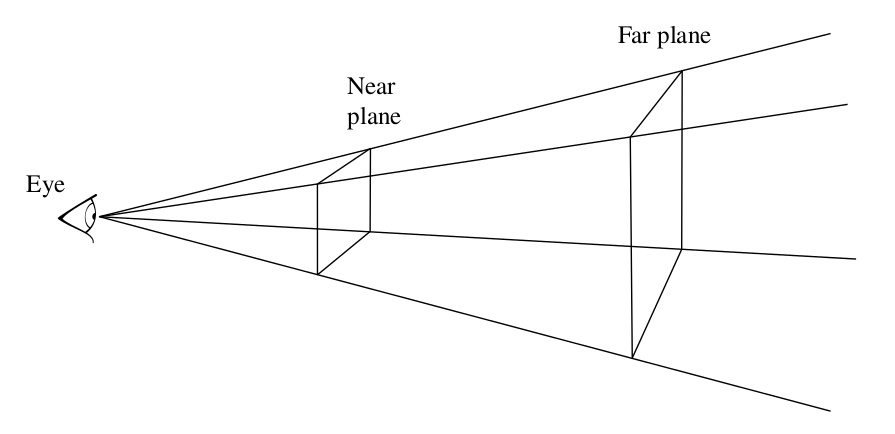
\includegraphics[width=0.7\textwidth]{imagenes/figura1_1}
  \end{minipage}}
  \fbox{\begin{minipage}{\dimexpr \textwidth-2\fboxsep-2\fboxrule}
    \abovecaptionskip=0pt
    \caption{The caption text}
  \end{minipage}}
\end{figure}

La cámara estenopeica puede ser simulada haciendo una abstracción y suponiendo que el papel de película se encuentra a cierta distancia en la dirección en la que la cámara está apuntando. Tal y como podemos ver en la figura 1.1, uniendo la posición dónde se encuentra la cámara con los filos de la película (near plane) se obtiene una región del espacio con forma de pirámide, que será la región del espacio que será captada en la imagen final. Sin embargo falta determinar que color tendrá la imagen en cada uno de sus píxeles. Para ello se traza un número concreto de rayos que pasan por cada píxel y a continuación se calcula la cantidad de luz que viaja a través de cada rayo trazado, lo cual constituye el principal problema a resolver dentro de los ray tracers. Por último se hace una media de los rayos que pasan por cada píxel para calcular su color.

El modelo de cámara recién presentado, a pesar de ser muy usado dentro de la renderización por ordenador, está bastante alejado del funcionamiento de una cámara actual, por lo que es deseable un modelo más complejo dentro de un renderizador fotorrealista. Esto se consigue simulando la utilización de múltiples lentes que nos permiten conseguir diversos efectos en la imagen final. Por otro lado, es común utilizar un parámetro temporal asociado a los rayos trazados, trazando varios rayos a lo largo del tiempo. La posición de los objetos de la escena puede cambiar en el tiempo, con lo que de esta manera se puede simular que ciertos objetos estén en movimiento al momento de tomar la fotografía. 


Aunque puedan utilizarse modelos de cámara más complejos, todos coinciden en que su principal tarea es determinar el espacio dentro de la escena que será captado en la imagen y trazar los rayos correspondientes a cada píxel.

\subsection{Intersección de rayos con objetos de la escena}

Una vez los rayos son trazados por la cámara, estos interseccionarán con objetos de la escena. La primera tarea del renderizador es ser capaz de calcular el punto en que cada rayo intersecciona con la escena, así como calcular las propiedades geométricas locales del objeto interseccionado.

\subsection{Visibilidad}

Recordemos que el objetivo es calcular la cantidad de luz que viaja por cada rayo que llega a la película de la cámara, o lo que es lo mismo, si consideramos el punto dónde el rayo intersecciona con la escena, calcular la cantidad de luz que viaja desde dicho punto en dirección a la cámara. Este proceso de calcular el color que se percibe de un punto de la escena se conoce como \emph{sombreado} o \emph{shading}.

Para calcular la cantidad de luz que es reflejada desde un punto en una dirección, primero es necesario estimar la cantidad de luz que llega a él. Por tanto es esencial que el renderizador sea capaz de determinar si una fuente de luz es visible desde el punto de la escena que está siendo sombreado.

\subsection{Distribución de la dispersión de la luz en superficies}

Llegados a este punto vemos que la forma en que los objetos de la escena reflejan y transmiten la luz que les llega es de gran importancia. Esto depende de las características de la materia que compone el objeto. La función que describe la forma en que los objetos de la escena reflejan la luz que reciben se denomina \emph{función de distribución de reflectancia bidireccional} o \emph{BRDF} (\emph{bidirectional reflectance distribution function}), y la notaremos por:
$$f_r:\mathds{R}^3\times \mathds{S}^2 \times \mathds{S}^2 \rightarrow \mathds{R}^+_0$$

Dónde notamos por $\mathds{S}^2$ a la esfera unidad de $\mathds{R}^3$. De esta manera, sea $p$ un punto en la superficie de un objeto, $\omega _i$ la dirección de un rayo incidente, y $\omega _o$ la dirección de un rayo reflejado, entonces la cantidad de energía reflejada por la superficie del objeto en el punto $p$ desde la dirección $\omega _i$ hacia la dirección $\omega _o$ es $f_r(p,\omega _o, \omega _i)$. Obviamente al tratarse de energía reflejada, si consideramos la esfera cuyo polo norte es la normal en $p$ a la superficie (notada como $n$ en la figura 1.2), si $\omega _i$ se encuentra en el hemisferio inferior de dicha esfera entonces $f_r(p,\omega _o, \omega _i)$ será igual a 0.\\

\begin{figure}[h]
  \lineskip=-\fboxrule
  \fbox{\begin{minipage}{\dimexpr \textwidth-2\fboxsep-2\fboxrule}
    \centering
    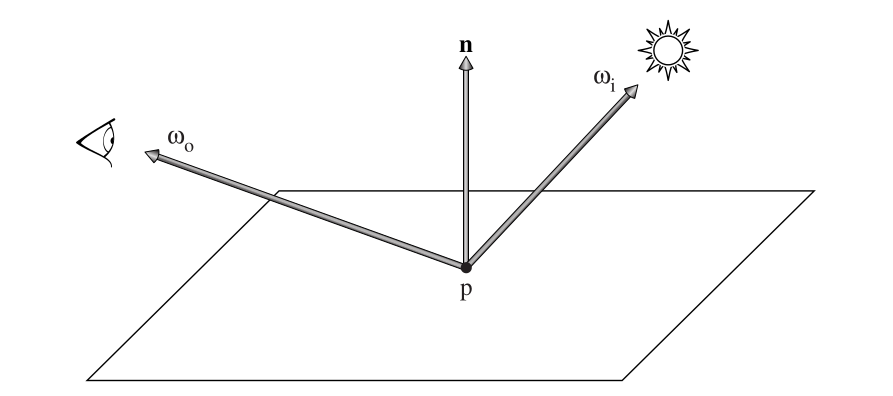
\includegraphics[width=0.7\textwidth]{imagenes/figura1_2}
  \end{minipage}}
  \fbox{\begin{minipage}{\dimexpr \textwidth-2\fboxsep-2\fboxrule}
    \abovecaptionskip=0pt
    \caption{The caption text}
  \end{minipage}}
\end{figure}

De manera similar podemos definir la función que describe la cantidad de energía transmitida, es decir, la cantidad de energía que atraviesa el objeto y escapa en una dirección. A dicha función la llamaremos \emph{función de distribución de transmitancia bidireccional} o \emph{BTDF} (\emph{bidireccional tramittance distribution function}) y la notamos por $f_t$.

Por último consideramos la función que describe de manera conjunta la energía reflejada y transmitida, la \emph{función de distribución de dispersión bidireccional} o \emph{BSDF} (\emph{bidirectional scattering distribution function}) que notamos por $f$.

En el caso de un objeto que presente reflexión especular perfecta, el BSDF en su superficie se puede describir de manera sencilla, ya que dada una dirección $\omega _i$, toda la luz procedente de esa dirección será reflejada en una única dirección saliente $\omega _o$, que será aquella que forme el mismo ángulo con la normal a la superficie que $\omega _i$. Este sería el caso de un espejo perfecto. Sin embargo la mayor parte de objetos de la vida real no se comportan de esta manera, por lo que en un ray tracer habrá diversos modelos que simulen diferentes materiales.

\subsection{Distribución de la luz}

La radiometría y la óptica geométrica nos otorgan las herramientas físicas y matemáticas que necesitamos para describir el comportamiento de la luz, y forman la base de la mayor parte de algoritmos utilizados en ray-tracing. La radiometría es la ciencia que trata la medición de radiación electromagnética, ya sea visible o no. La óptica geométrica tiene en cuenta propiedades macroscópicas de la luz, que son suficientes para describir la forma en que la luz interacciona con objetos mucho más grandes que su longitud de onda. Por otra parte, no es raro simular fenómenos propios de la óptica física, aunque en nuestro caso no tendremos en cuenta este tipo de fenómenos. Hay una serie de asunciones que haremos acerca del comportamiento de la luz para simplificar el cálculo de la energía radiante en la escena:

\begin{itemize}
\item Linealidad: El efecto combinado de dos entradas en un sistema óptico es siempre igual a la suma del efecto de cada una de las entradas individualmente.
\item Conservación de la energía: La energía radiante reflejada o transmitida por una superficie nunca será mayor que la energía incidente sobre dicha superficie.
  \item Estado de reposo: Se asume que la distribución de la luz en la escena ha alcanzado el equilibrio, por lo que no habrá cambios en la distribución de la radiancia a lo largo del tiempo.
\end{itemize}

Antes de presentar las magnitudes radiométricas centrales en renderización, vamos a definir el concepto de \emph{ángulo sólido}.

\subsubsection*{Ángulo sólido}

Como ya sabemos, en una circunferencia de radio unidad, el ángulo en radianes entre dos radios es igual a la longitud de circunferencia comprendida entre ellos (figura 1.3). Conceptualmente, el ángulo sólido se trata de una extensión de los ángulos planos a $\mathds{R}^3$, y mide el tamaño con el que se ve un objeto desde un punto. Podemos entender un objeto como una superficie simple, regular a trozos y orientable.

\begin{definicion}
  Consideremos un punto $P \in \mathds{R}^3$ y sea $A \subseteq \mathds{R}^3/\{P\}$ una superficie simple, regular a trozos y orientable. Se denomina ángulo sólido subtendido por $A$ desde $P$ a la región del espacio $\{P + \lambda (V-P) \in \mathds{R}^3 : \lambda \in (0,1], V \in A\}$, y se nota por $\Omega(A)$. 
\end{definicion}

\begin{definicion}
    Sea $P \in \mathds{R}^3$ y consideremos la esfera unidad con centro $P$, $\mathcal{B}(P,1)$. Sea $\pi :\mathds{R}^3/\{P\}\rightarrow \mathcal{B}(P,1)$ la proyección sobre la esfera $\mathcal{B}(P,1)$, es decir, $\pi(r) = P + \frac{r-P}{\|r-P\|}$. Sea $A \subseteq \mathds{R}^3/\{P\}$ una superficie simple, regular a trozos y orientable, y tomamos $I = \int _{\pi(A)} dS$. Entonces diremos que el ángulo sólido subtendido por $A$ desde $P$ mide $I$ estereorradianes.
\end{definicion}

\begin{figure}[h]
  \lineskip=-\fboxrule
  \fbox{\begin{minipage}{\dimexpr \textwidth-2\fboxsep-2\fboxrule}
    \centering
    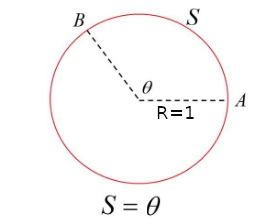
\includegraphics[width=0.3\textwidth]{imagenes/figura1_5}
  \end{minipage}}
  \fbox{\begin{minipage}{\dimexpr \textwidth-2\fboxsep-2\fboxrule}
    \abovecaptionskip=0pt
    \caption{The caption text}
  \end{minipage}}
\end{figure}

\begin{figure}[h]
  \lineskip=-\fboxrule
  \fbox{\begin{minipage}{\dimexpr \textwidth-2\fboxsep-2\fboxrule}
    \centering
    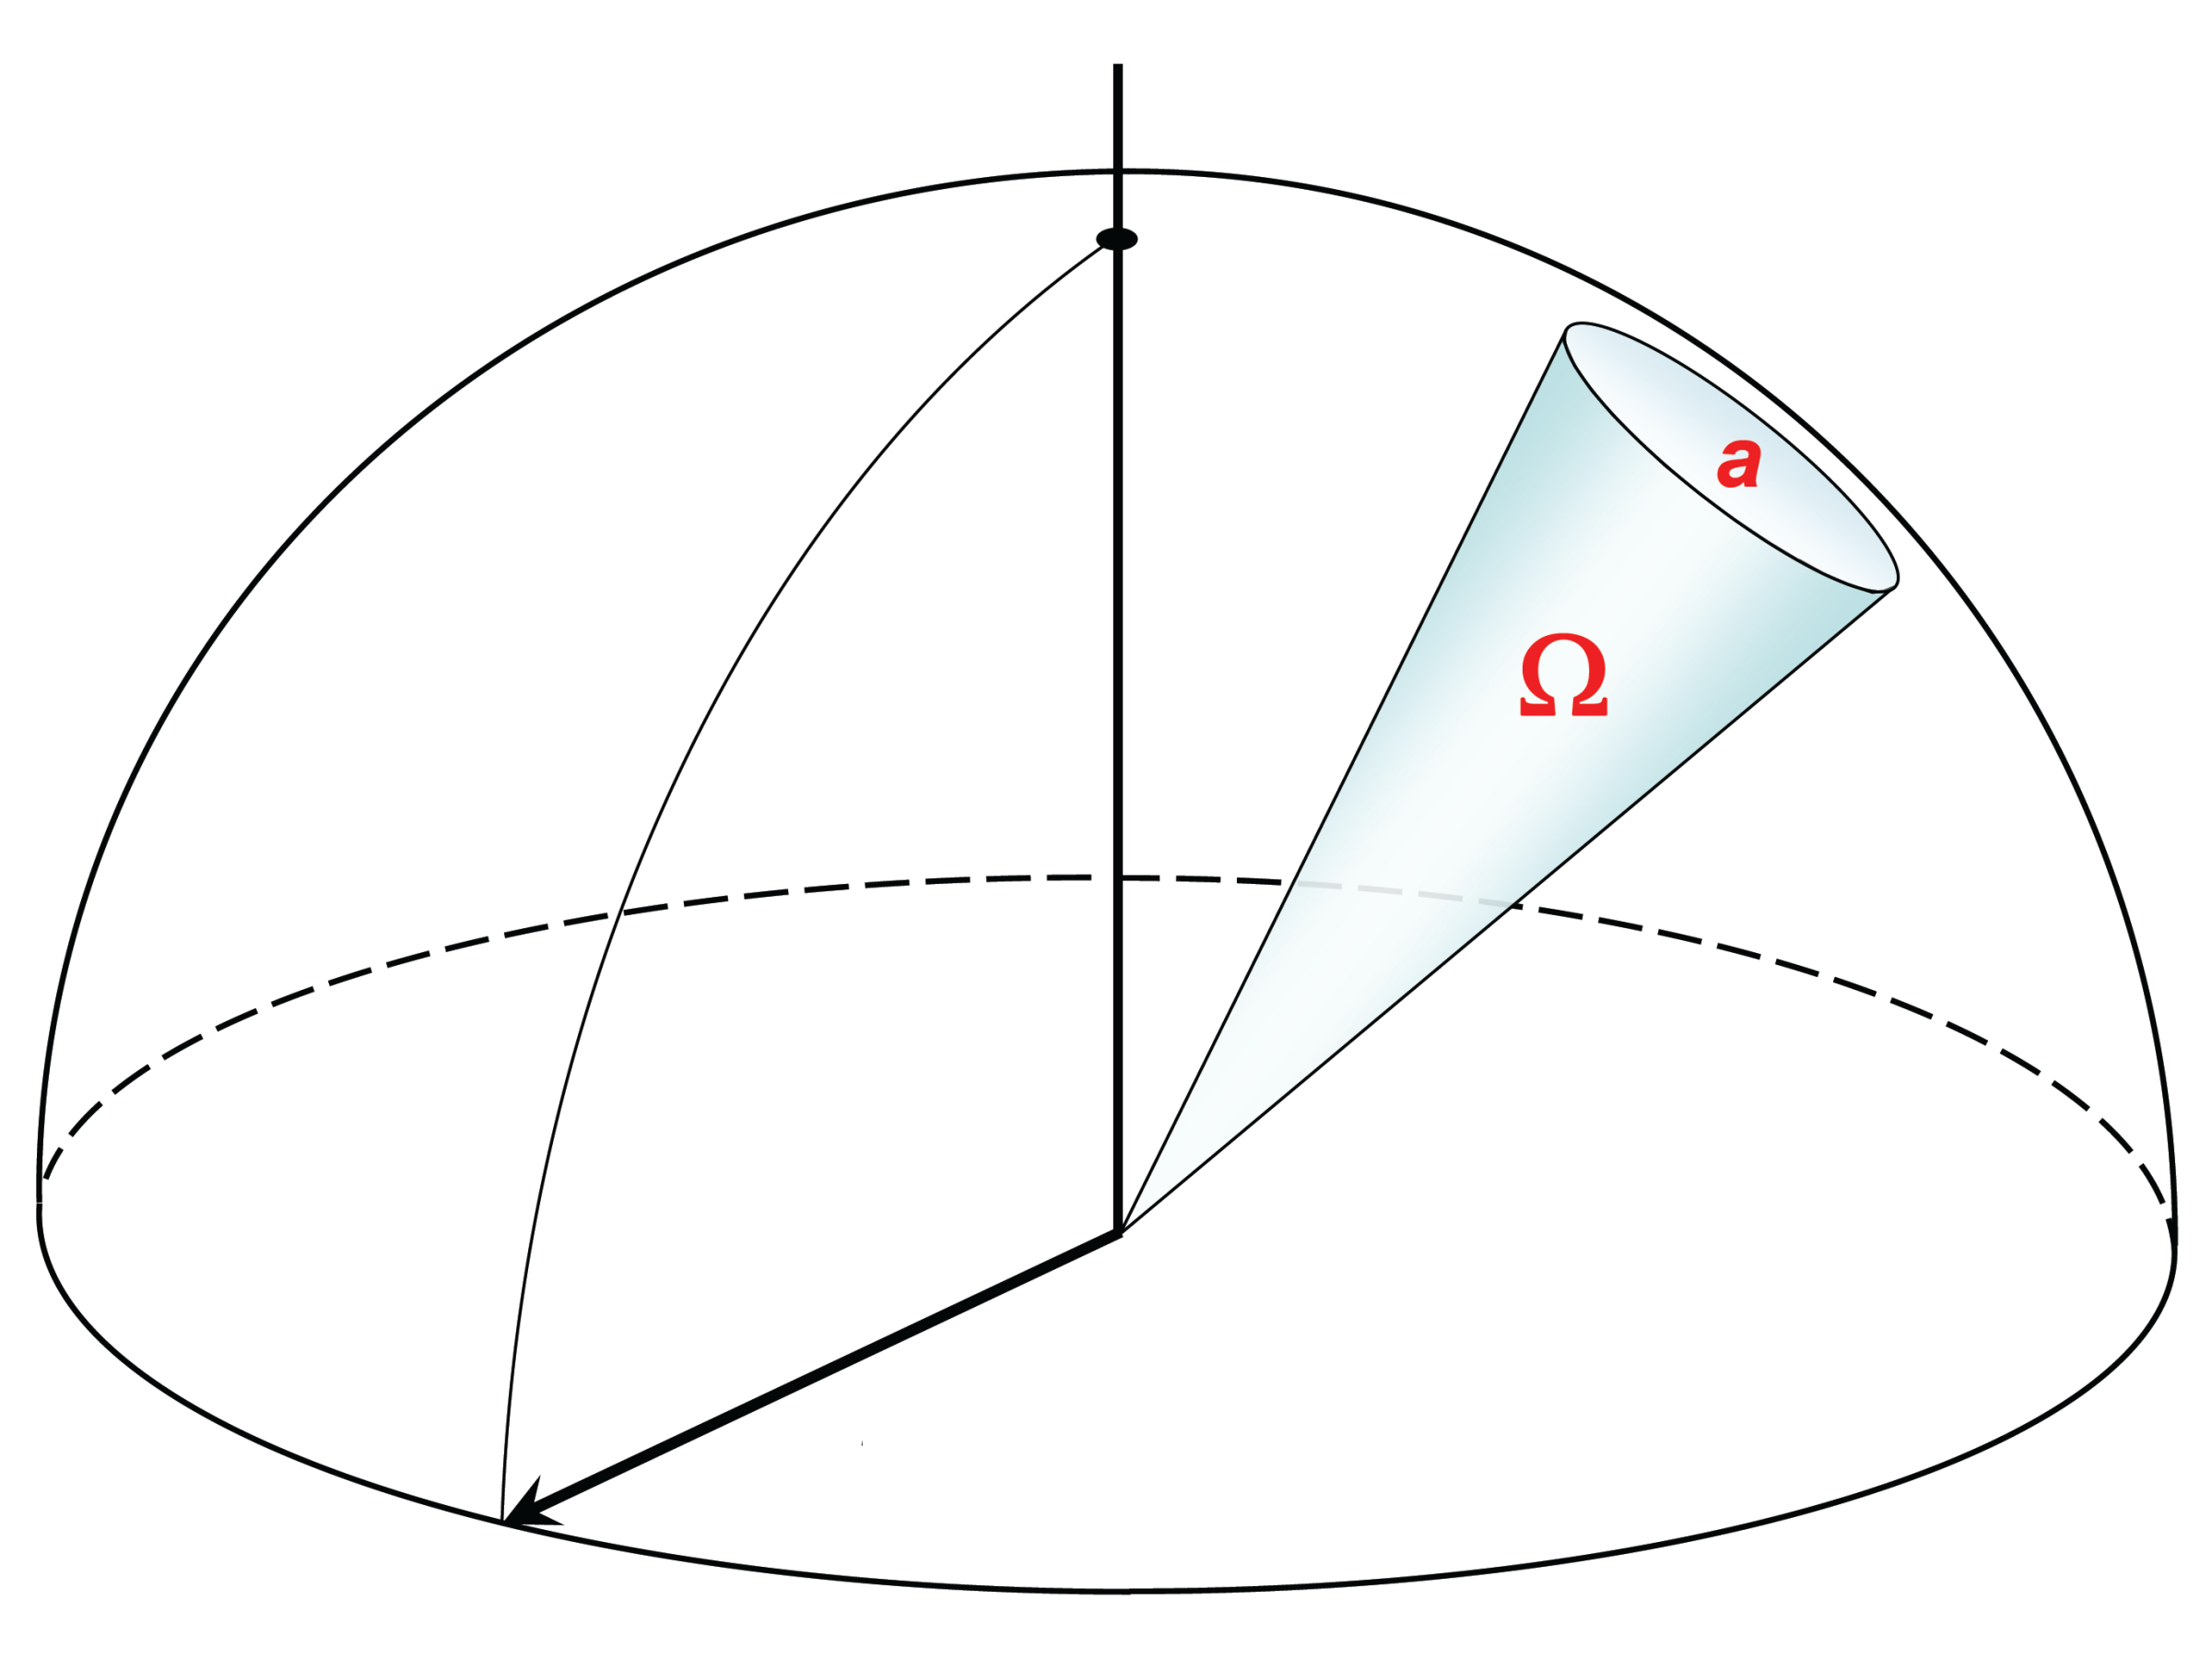
\includegraphics[width=0.6\textwidth]{imagenes/figura1_4}
  \end{minipage}}
  \fbox{\begin{minipage}{\dimexpr \textwidth-2\fboxsep-2\fboxrule}
    \abovecaptionskip=0pt
    \caption{The caption text}
  \end{minipage}}
\end{figure}

En la definición anterior hemos usado $dS$ para denotar la integral de superficie. Como vemos el ángulo sólido subtendido por un objeto claramente depende del punto de referencia $P$. Sin embargo, supongamos que queremos medir el ángulo sólido subtendido por un objeto desde un punto $P$. En renderización se trabaja con $\mathds{R}^3$ como espacio afín, por lo que podemos aplicar una traslación del marco de referencia para situar $P$ en el origen de coordenadas. Por tanto, a efectos prácticos siempre podemos suponer que trabajamos en la esfera unidad $\mathds{S}^2$. Vamos a definir ahora la función que mide el ángulo sólido en la esfera unidad:

\begin{definicion}
  Sea $\mathscr{S}$ la familia de superficies simples contenidas en la esfera unidad $\mathds {S}^2$, definimos la función $\mu :\mathscr{S} \rightarrow \mathds{R}^+_0$ como:
  $$\mu(C) = \int_C \text{ }dS , \hspace{0.5cm} \forall C\in \mathscr{S}$$

  La función $\mu$ mide el ángulo sólido subtendido por cada superficie simple de la esfera.
\end{definicion}

Vamos ahora a derivar una serie de resultados básicos relacionados con el ángulo sólido que nos serán útiles durante el resto de trabajo. Consideremos la parametrización de la esfera unidad $\Theta:[0,\pi ]\times [0,2\pi ]\rightarrow \mathds{R}^3$, con:
$$\Theta(\theta ,\varphi ) = ( \sin \theta \cos \varphi,  \sin \theta \sin \varphi , \cos \theta),\hspace{0.5cm}  \forall (\theta , \varphi)\in [0,\pi ]\times [0,2\pi ]$$

Derivando parcialmente $\Theta$ y calculando el producto vectorial de sus derivadas parciales vemos que:
$$\Theta _\theta(\theta ,\varphi ) = \frac{\partial \Theta}{\partial \theta}(\theta ,\varphi ) = (\cos\theta\cos\varphi, \cos\theta\sin\varphi, -\sin\theta)$$

$$\Theta _\varphi(\theta ,\varphi ) = \frac{\partial \Theta}{\partial \varphi}(\theta ,\varphi ) = (-\sin\theta\sin\varphi, \sin\theta\cos\varphi, 0)$$

$$\Theta _\theta(\theta ,\varphi )\times \Theta _\varphi(\theta ,\varphi ) = (\sin^2\theta\cos\varphi,\sin^2\theta\sin\varphi,\sin\theta\cos\theta)$$

Con lo que concluimos que:
\begin{align*}
\mu (C) = \int_C \text{ }dS &= \iint_{\Theta^{-1}(C)}\|\Theta _\theta(\theta ,\varphi )\times \Theta _\varphi(\theta ,\varphi )\| d\theta d\varphi \\
&= \iint_{\Theta^{-1}(C)} \sin\theta d\theta d\varphi \hspace{1cm} \forall C \in \mathscr{S}
\end{align*}

De aquí en adelante, por comodidad, notaremos por $\pi$ a la proyección sobre la esfera unidad $\mathds{S}^2$, es decir, $\pi(p)=\frac{p}{\|p\|}$, $\forall p \in \mathds{R}^3/\{(0,0,0)\}$. Pasamos ahora a demostrar la siguiente proposición:

\begin{proposicion}\label{angSolido1}
  Sea $\mu$ la medida del ángulo sólido, y sea $C$ una superficie en $\mathds{R}^3/\{(0,0,0)\}$ simple, regular a trozos y orientable, tal que cada recta que empiece en el origen y acabe en un punto de $C$ sólo interseccione con $C$ una vez. Consideramos la función $g:\mathds{R}^3/\{(0,0,0)\} \rightarrow \mathds{R}^3$, con $g(p)=\frac{p}{\|p\|^3}$. Entonces se cumple que:

 \begin{equation}
 \mu (\pi(C)) = \int _C g \text{ }dS 
 \end{equation}
 
\end{proposicion}

\begin{figure}[h]
  \lineskip=-\fboxrule
  \fbox{\begin{minipage}{\dimexpr \textwidth-2\fboxsep-2\fboxrule}
    \centering
    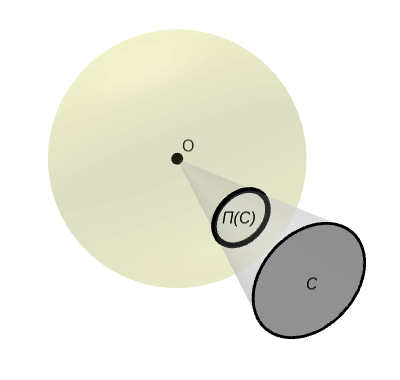
\includegraphics[width=0.6\textwidth]{imagenes/figura1_6}
  \end{minipage}}
  \fbox{\begin{minipage}{\dimexpr \textwidth-2\fboxsep-2\fboxrule}
    \abovecaptionskip=0pt
    \caption{The caption text}
  \end{minipage}}
\end{figure}


\begin{proof}

Sea $C_r$ la porción del espacio comprendida entre $C$ y $\pi (C)$, y sea $\partial C_r$ su frontera. Sea $C_p = \partial C_r /(C\cup \pi(C))$ la superficie que delimita lateralmente la región $C_r$. Vamos ahora a calcular la divergencia de $g$. Sea $(x,y,z)\in \mathds{R}^3$:

\begin{align*}
  \textrm{div } g (x,y,z) &= \frac{\partial g}{\partial x}(x,y,z) + \frac{\partial g}{\partial y}(x,y,z) + \frac{\partial g}{\partial z} (x,y,z) =\\
  & = \frac{(x^2+y^2+z^2)^{\frac{3}{2}}-3x^2(x^2+y^2+z^2)^{\frac{1}{2}}}{(x^2+y^2+z^2)^3} +\\
  & + \frac{(x^2+y^2+z^2)^{\frac{3}{2}}-3y^2(x^2+y^2+z^2)^{\frac{1}{2}}}{(x^2+y^2+z^2)^3} +\\
  &+ \frac{(x^2+y^2+z^2)^{\frac{3}{2}}-3z^2(x^2+y^2+z^2)^{\frac{1}{2}}}{(x^2+y^2+z^2)^3} = 0
\end{align*}

Y, por tanto, aplicando el teorema de divergencia tenemos que:

$$\int _{\partial C_r}g\text{ } dS = \iiint _{C_r}\text{div } g \text{ }dx dy dz = 0$$

Sea $C_p = \bigcup _{i=1}^n S_i$ una descomposición finita de $C_p$ como unión de superficies simples y regulares. Fijado $i\in \{1\ldots n\}$, sea $\Psi^i : W^i \rightarrow \mathds{R}^3$ una parametrización simple y suave de $S_i$ orientada mediante la normal exterior, y sean $\Psi^i_u$, $\Psi^i_v$ sus derivadas parciales. Es fácil ver que dado un punto $P\in S_i$, se tiene que el vector que va desde el origen hasta $P$ es perpendicular a la normal a $S_i$ en $P$. Por tanto tenemos que:

$$ \int_{S_i} g\text{ }dS = \iint _{W^i} \frac{<\Psi^i(u,v) | (\Psi^i_u(u,v)\times \Psi^i_v (u,v))>}{\|\Psi^i(u,v)\|^3}\text{ } du dv = 0$$


Dónde se ha usado que $<\Psi^i(u,v) | (\Psi^i_u(u,v)\times \Psi^i_v (u,v))> = 0$, $\forall (u,v)\in W^i$, ya que el producto vectorial de las derivadas parciales es igual a la normal a la superficie y el producto escalar de vectores perpendiculares es nulo. Sabemos que $\partial C_i = C\cup \pi(C) \cup C_p$, y usando las dos igualdades anteriores tenemos que:

$$0 = \int _{\partial C_r}g\text{ } dS = \int _{C}g\text{ } dS + \int _{\pi(C)}g\text{ } dS $$

Sea $\Phi :W\rightarrow \mathds{R}^3$, una parametrización simple y suave de $\pi (C)$ orientada con la normal exterior, y sean $\Phi _u$, $\Phi _v$ sus derivadas parciales. Como $\pi (C)$ está contenido en la esfera unidad, para todo $(u,v)\in W$ se cumple que $-\Phi(u,v) = \frac{\Phi_u(u,v)\times \Phi_v (u,v)}{\|\Phi_u(u,v)\times \Phi_v (u,v)\|}$ y que  $\|\Phi(u,v)\| = 1$, y por ello:

\begin{align*}
  \int _{\pi(C)}g\text{ } dS &= \iint _{W} \frac{<\Phi(u,v) | (\Phi_u(u,v)\times \Phi_v (u,v))>}{\|\Phi(u,v)\|^3}\text{ } du dv =\\
  &= - \iint _{W} \frac{\|\Phi_u(u,v)\times \Phi_v (u,v)\|}{\|\Phi(u,v)\|^2}\text{ } du dv = - \int _{\pi(C)}\text{ } dS
\end{align*}

Y por tanto deducimos que:

\begin{align*}
  & 0 = \int _{C}g\text{ } dS + \int _{\pi(C)}g\text{ } dS = \int _{C}g\text{ } dS - \int _{\pi(C)}\text{ } dS \Rightarrow \\
  & \Rightarrow \int _{C}g\text{ } dS = \int _{\pi(C)}\text{ } dS = \mu (\pi(C))
\end{align*}

Tal y como queríamos.\\
\end{proof}

Podemos ahora introducir un concepto bastante natural por la forma en que hemos definido la función $\mu$.

\begin{definicion}
  Sea $C\subseteq \mathds{S}^2$ una superficie simple y sea $h: C\rightarrow \mathds{R}$ un campo escalar, $i: C\rightarrow \mathds{R}^3$ un campo vectorial. Entonces la integral respecto al ángulo sólido de las funciones $h$ e $i$ se define como:

  $$\int _C h\text{ } d\mu = \int _C h\text{ } dS$$

   $$\int _C i\text{ } d\mu = \int _C i\text{ } dS$$
  
\end{definicion}

Y por último podemos generalizar la proposición \ref{angSolido1} de la siguiente manera:

\begin{proposicion}\label{ToArea}
Sea $C$ una superficie en $\mathds{R}^3/\{(0,0,0)\}$ simple, regular a trozos y orientable, tal que cada recta que empiece en el origen y acabe en un punto de $C$ sólo interseccione con $C$ una vez. Sea $h: \mathds{S}^2\rightarrow \mathds{R}^+_0$ un campo escalar no negativo. Consideramos la función $g:\mathds{R}^3/\{(0,0,0)\} \rightarrow \mathds{R}^3$, con $g(p)=\frac{p}{\|p\|^3}$. Entonces se cumple que:

 \begin{equation}\label{transfToArea}
   \int_{\pi(C)} h\text{ }d\mu = \int _C (h\circ \pi) g \text{ }dS 
 \end{equation}
 
  \end{proposicion}

\subsubsection*{Medida de la luz}

Una vez nos hemos familiarizado con el concepto de ángulo sólido, vamos a presentar una serie de magnitudes radiométricas básicas. Todas estas magnitudes dependen de la longitud de onda, y aunque obviaremos esto, es importante tenerlo en cuenta.

\begin{itemize}
\item \textbf{Energía radiante}: Las fuentes de luz emiten fotones, cada uno de los cuales porta una cantidad de energía que depende de la longitud de onda. La energía se mide en julios (j), y notaremos por $Q$ a la función que mide la energía en una región durante un periodo de tiempo.
\item \textbf{Flujo radiante}: La energía está medida sobre algún periodo de tiempo, y por tanto, bajo la asunción de estado de reposo, es más conveniente trabajar con magnitudes que se midan en un instante de tiempo. El flujo radiante se define como la cantidad total de energía por unidad de tiempo que atraviesa una región. Se mide en vatios (W), y notaremos por $\Phi$ a la función que mide el flujo radiante en una región.
\item \textbf{Irradiancia y emitancia radiante}: Las dos magnitudes miden el flujo radiante por unidad de superficie, en el caso de la irradiancia se mide el flujo llegando a la superficie, y en el caso de la emitancia radiante se mide el flujo saliendo de la superficie. Se mide en vatios por metro cuadrado (W/m$^{-2}$) y notaremos por $E$ a la función que mide la irradiancia.

\item \textbf{Radiancia incidente y saliente}: Se trata de la magnitud que más utilizaremos. La irradiancia nos da una medida del flujo radiante por unidad de superficie, pero no tiene en cuenta que el flujo tiene una distribución direccional, es decir, la cantidad de flujo que llega a una superficie varía según la dirección del flujo incidente. La radiancia mide el flujo por unidad de superficie proyectada y por unidad de ángulo sólido. Cuando hablamos de superficie proyectada nos referimos a que calculamos el flujo en una superficie hipotética que es perpendicular a la dirección del flujo incidente/saliente. Se mide en vatios por estereorradián por metro cuadrado (W sr$^{-1}$ m$^{-2}$) y notaremos por $L: \mathds{R}^3 \times \mathds{S}^2\rightarrow \mathds{R}^+_0$ a la función que mide la radiancia.

  Notemos por $\mathcal{H}^2(n)$ al hemisferio superior de la esfera unidad cuyo polo norte es el vector $n$. Si consideramos una superficie con normal $n$ en un punto $p$, la radiancia generalmente no es continua en $p$. Por tanto tiene sentido distinguir entre la función radiancia encima de la superficie y debajo de ella:

  $$L^+(p,\omega) = \lim_{t\rightarrow 0^+} L(p+tn, \omega)$$
  $$L^-(p,\omega) = \lim_{t\rightarrow 0^-} L(p-tn, \omega)$$

  Podemos definir por tanto las funciones de radiancia incidente y radiancia saliente como sigue (siempre consideramos que la dirección $\omega$ apunta hacia fuera de la superficie, aunque sea radiancia incidente):

  \[ L_i(p,\omega) = 
   \begin{cases} 
      L^+(p,- \omega ),  & \omega \cdot n > 0 \\
      L^-(p,- \omega ),  & \omega \cdot n < 0
   \end{cases}
  \] 
  \\
  \[L_s(p,\omega) = 
   \begin{cases} 
      L^+(p, \omega ),  & \omega \cdot n > 0 \\
      L^-(p,\omega ),  & \omega \cdot n < 0
   \end{cases}
  \] 
  
\end{itemize}

Por como están definidas las magnitudes anteriores tenemos las siguientes relaciones entre ellas:

\begin{itemize}
\item La irradiancia en un punto $p\in \mathds{R}^3$ perteneciente a una superficie con normal $n$ en $p$ cumple que:
  $$ E(p) = \int _{\mathds{S}^2} L_i(p,\omega ) |n \cdot \omega| \text{ } d\mu(\omega )$$

  Dónde se multiplica por $| n\cdot \omega |$ debido al hecho de que la radiancia se mide respecto a la superficie proyectada. Notar que $| n\cdot \omega |$ es igual al coseno del ángulo que forman.

\item El flujo en una superficie $A\subseteq \mathds{R}^3$ cumple que:
  $$\Phi (A)= \int _A E\text{ }dS$$
\end{itemize}

Por último, la radiancia saliente de una superficie en un punto $p \in \mathds{R}^3$ y en una dirección $\omega _o \in \mathds{S}^2$ a causa de la iluminación incidente en $p$ se puede calcular como sigue, con $n$ la normal a la superficie en $p$:
\begin{equation}\label{dispersion}
L_s(p,\omega _o) = \int _{\mathds{S}^2}f(p,\omega _o, \omega _i) L_i(p, \omega _i) |n\cdot \omega _i|\text{ }d\mu (\omega _i)
\end{equation}

donde $f$ es la $BDSF$ descrita en el apartado anterior. Esta ecuación se conoce como ecuación de dispersión. Si además la superficie es emisiva en el punto $p$, tenemos que la radiancia saliente total en el punto $p \in \mathds{R}^3$ y en una dirección $\omega _o \in \mathds{S}^2$ se calcula como:
\begin{equation}\label{renderingEquation}
L_s(p,\omega _o) = L_e(p,\omega_o) + \int _{\mathds{S}^2}f(p,\omega _o, \omega _i) L_i(p, \omega _i) |n\cdot \omega _i|\text{ }d\mu (\omega _i)
\end{equation}

dónde la función $L_e(p, \omega_o)$ describe la radiancia emitida en el punto $p$ y en la dirección $\omega_o$. Esta ecuación se denomina \emph{ecuación de renderización}, o \emph{rendering equation}, y es fundamental en ray-tracing, ya que es la ecuación utilizada para estimar el color de los puntos con los que interseccionan los rayos trazados por la cámara, estimando el valor de radiancia saliente en dirección a la cámara en el punto de intersección. La complejidad de la integral dependerá de la escena que estemos renderizando, y como podemos intuir no tiene una solución analítica. En el capítulo 3 abordaremos diferentes formas de aproximar esta ecuación.

Hay que destacar que el algoritmo de ray-tracing tiene una naturaleza recursiva, ya que con el objetivo de estimar el color de un punto, se trazarán rayos desde ese punto en direcciones dónde el valor de radiancia incidente o de BDSF sea grande. Dicho rayo puede volver a interseccionar con otro componente de la escena, del cuál tendremos que estimar a su vez la radiancia saliente en dirección al punto inicial.

\subsection{Propagación de los rayos}

En todo lo descrito con anterioridad hemos supuesto que los rayos se propagan por el vacío, por lo que la energía radiante que viaja por ellos no se ve atenuada. Sin embargo en la vida real ciertos componentes ambientales como la niebla o el humo invalidan dicha suposición. Es por ello que es habitual que los ray tracers simulen este tipo de efectos ambientales, dónde la energía radiante se ve atenuada al viajar por el espacio en presencia de partículas en suspensión. No obstante, en lo referente a los objetivos de este trabajo podemos obviar este tipo de efectos.

\section{Concepto de método de Monte Carlo y su relación con el ray-tracing}

Los métodos de Monte Carlo son un conjunto de algoritmos basados en el muestreo aleatorio. Sus objetivos son:

\begin{itemize}
\item Sea $(\Gamma, \mathcal{A}, P)$ un espacio probabilístico, sea $X:\Gamma \rightarrow \mathds{R}^n$ una variable o un vector aleatorio y sea $P_X$ su distribución de probabilidad, generar un conjunto de muestras $\{x^{(r)}\}_{r=1}^R$ independientes que sigan dicha distribución. 
\item Estimar la esperanza de determinadas funciones bajo dicha distribución, es decir, sea $g$ una función mebible definida sobre $(\mathds{R}^n, \mathscr{B}^n)$, estimar el valor de:
$$ E[g(X)] = \int g(s)\text{ }dP(s)$$
\end{itemize}

Vemos que una vez resolvamos el primer problema, podemos usar el siguiente estimador para resolver el segundo:
\begin{equation}\label{estMC}
\overset{\wedge}{g} = \frac{1}{R}\sum_{r=1}^R g(x^{(r)})
\end{equation}

Ya que es claro que si las muestras $\{x^{(r)}\}_{r=1}^R$ son independientes y siguen la distribución $P_X$, entonces la esperanza del estimador cumple que:
$$E[\overset{\wedge}{g}] = E[\frac{1}{R}\sum_{r=1}^R g(x^{(r)})] = \frac{1}{R}\sum_{r=1}^R E[g(x^{(r)})] = \frac{1}{R} R E[g(X)] = E[g(X)]$$

Al estimador definido en \ref{estMC} lo llamaremos estimador Monte Carlo de $g$. Habitualmente trabajaremos con vectores aleatorios continuos, así que salvo que se especifique lo contrario, así lo supondremos. Supongamos ahora que queremos estimar la integral de una función $h:K\rightarrow \mathds{R}$ en lugar de su esperanza. Sea $X:\Gamma \rightarrow K$ un vector aleatorio tal que su función de densidad $f_X$ cumple que $f_X(s)\neq 0$ para todo $s$ tal que $|h(s)|>0$, y sea $\{x^{(r)}\}_{r=1}^R$ un conjunto de muestras indepentientes siguiendo la distribución de probabilidad de $X$. Entonces para aproximar la integral de $h$ podemos utilizar el estimador Monte Carlo de la función $g = \frac{h}{f_X}$:

$$\overset{\wedge}{g} = \frac{1}{R}\sum_{r=1}^R \frac{h(x^{(r)})}{f_X(x^{(r)})}$$

En efecto la esperanza de $\overset{\wedge}{g}$ es igual a la integral de $h$ en $K$:

\begin{align*}
E[\overset{\wedge}{g}] &= E[\frac{1}{R}\sum_{r=1}^R \frac{h(x^{(r)})}{f_X(x^{(r)})}] = \frac{1}{R}\sum_{r=1}^R E[\frac{h(x^{(r)})}{f_X(x^{(r)})}] =\\
&= \frac{R}{R}  \int _K \frac{h(x)}{f_X(x)}f_X(x) \text{ }dx = \int _K h(x) \text{ }dx
\end{align*}

La elección de la distribución de probabilidad respecto a la que tomamos las muestras es clave, ya que seleccionar una distribución de probabilidad que asigne mayores probabilidades a los puntos donde la función $g$ es mayor supone una importante técnica para reducir la varianza del estimador.

Los métodos de Monte Carlo son una importante herramienta dentro del ray-tracing. El motivo de que estos métodos sean más efectivos en renderización que otras técnicas de integración numérica es que la varianza del estimador es independiente de la dimensionalidad del espacio muestreado. En efecto, sean $\{x^{(r)}\}_{r=1}^R$ un conjunto de muestras independientes siguiendo la distribución de probabilidad de $X$, y supongamos que $E[g(X)^2]< +\infty$. Entonces tenemos que:
\begin{align*}
\Var(\overset{\wedge}{g}) &= \Var(\frac{1}{R}\sum_{r=1}^R g(x^{(r)})) = \frac{1}{R^2}\Var(\sum_{r=1}^R g(x^{(r)})) \\
&= \frac{1}{R^2}\sum_{r=1}^R \Var(g(x^{(r)})) = \frac{1}{R} \Var(g(X))
\end{align*}

Esto muestra que la varianza del estimador decrece con un ratio de $\frac{1}{R}$, dónde $R$ es el número de muestras.

Estos métodos son utilizados, entre otras cosas, para estimar el valor de la ecuación de dispersión (\ref{dispersion}), de ahí su importancia.

\section{Objetivos}
El principal objetivo de este trabajo es estudiar el uso de métodos de Monte Carlo en renderizadores 3D físicamente realistas para estimar numéricamente la distribución de radiancia en el espectro visible dentro de la escena renderizada. Asimismo se estudiarán diferentes algoritmos descritos en la literatura que reducen la varianza del estimador Monte Carlo, obteniendo así mejores resultados sin tener que aumentar el número de muestras.




%
\titlespacing*{\subsection}
  {0pt}{2\baselineskip}{\baselineskip}

\chapter{Métodos de Monte Carlo}

Al final del capítulo anterior se mencionaron los problemas a los que pretenden poner solución los métodos de Monte Carlo. En este capítulo se demostrará la convergencia del estimador de Monte Carlo y se describirán diversos métodos de Monte Carlo con aplicación en renderización.

\section{Conceptos básicos}

Vamos a presentar una serie de conceptos que nos serán útiles posteriormente. Empezaremos por describir el concepto de proceso estocástico. Habitualmente se usa la letra $\Omega$ para referirse al espacio muestral en el que trabajamos, pero en nuestro caso usaremos $\Gamma$ para que no haya confusión con el concepto de ángulo sólido.

\begin{notacion}
Notaremos por $\mathscr{B}^n$ a la $\sigma$-álgebra de Borel en $\mathds{R}^n$.
\end{notacion}

\begin{definicion}[Proceso estocástico]
 Sea $(\Gamma, \mathcal{A}, P)$ un espacio probabilístico. Un proceso estocástico es una familia de variables o vectores aleatorios $\{X_t\}_{t\in T}$ definidos sobre $(\Gamma, \mathcal{A}, P)$ con valores en un espacio de Borel $(E, \mathscr{B}_E)$, con $E\subseteq \mathds{R}^n$. El conjunto $T$ se denomina espacio paramétrico y es un conjunto ordenado arbitrario, y el espacio $(E, \mathscr{B}_E)$ se denomina espacio de estados. 
\end{definicion}

\begin{definicion}
Sea $\{X_t\}_{t\in T}$ un proceso estocástico. Diremos que $\{X_t\}_{t\in T}$ es un proceso estocástico en tiempo discreto si $T$ es un conjunto discreto. Diremos que $\{X_t\}_{t\in T}$ es un proceso estocástico en tiempo continuo si $T$ es un conjunto no numerable. Diremos que $\{X_t\}_{t\in T}$ es un proceso estocástico real si el espacio de estados $(E,\mathscr{B}_E)$ cumple que $E\subseteq \mathds{R}$, es decir, si $\{X_t\}_{t\in T}$ es una sucesión de variables aleatorias.
\end{definicion}

\iffalse
\begin{notacion}
Notaremos por $(\mathds{R}^n)^T$ al conjunto de las funciones de $T$ en $\mathds{R}^n$.
\end{notacion}

\begin{definicion}[Trayectorias muestrales]
Sea $(\Gamma, \mathcal{A}, P)$ un espacio probabilístico. Sea $\{X_t\}_{t\in T}$ un proceso estocástico definido sobre $(\Gamma, \mathcal{A}, P)$. Fijado $\gamma \in \Gamma$, se denomina trayectoria muestral del proceso asociada a $\gamma$ a la función $\{X_t(\gamma)\}_{t\in T} \in (\mathds{R}^n)^T$, con $\{X_t(\gamma)\}_{t\in T}(t) = X_t(\gamma),\text{ }\forall t\in T$ . Definimos por tanto la siguiente función:

\begin{align*}
\mathcal{X}: &\Gamma \rightarrow (\mathds{R}^n)^T \\
&\gamma \rightarrow \mathcal{X}(\gamma) = \{X_t(\gamma)\}_{t\in T} 
\end{align*}

que asigna a cada $\gamma$ su trayectoria muestral.
\end{definicion}

\begin{definicion}[Clase de rectángulos medibles en $(\mathds{R}^n)^T$]
Un rectángulo de lados $B_1,\ldots , B_r \in \mathds{R}^n$ es un conjunto de la forma:

$$\{f\in (\mathds{R}^n)^T / f(t_1)\in B_1, \ldots , f(t_r)\in B_r;\text{ } t_i\in T,\text{ } \forall i \in \{1,\ldots ,r\}\}$$

Un rectángulo se denomina medible cuando sus lados son conjuntos medibles. Notaremos por $(\mathscr{F}^n)^T$ a la clase de todos los rectángulos medibles en $(\mathds{R}^n)^T$.
\end{definicion}

\begin{proposicion}
$(\mathscr{F}^n)^T$ es una semi-álgebra sobre $(\mathds{R}^n)^T$.
\end{proposicion}

\begin{notacion}
Notaremos por $(\mathscr{B}^n)^T$ a la $\sigma$-álgebra generada por la clase de rectángulos medibles $(\mathscr{F}^n)^T$.
\end{notacion}

\begin{teorema}
Sea $\{X_t\}_{t\in T}$ un proceso estocástico definido sobre el espacio probabilístico $(\Gamma , \mathcal{A}, P)$. Entonces la función $\mathcal{X}: (\Gamma , \mathcal{A}, P)\rightarrow ((\mathds{R}^n)^T,(\mathscr{B}^n)^T)$ es medible.
\end{teorema}

\begin{definicion}[Distribución de un proceso estocástico]
Sea $\{X_t\}_{t\in T}$ un proceso estocástico definido sobre $(\Gamma, \mathcal{A}, P)$. La distribución del proceso es la función $P_{\mathcal{X}}:(\mathscr{B}^n)^T\rightarrow [0,1]$ definida como:
$$P_{\mathcal{X}}(B) = P(\mathcal{X}^{-1}(B)), \text{ } \forall B\in (\mathscr{B}^n)^T $$
\end{definicion}
\fi

Pasamos ahora a definir el concepto de esperanza y probabilidad condicionada.

\begin{definicion}[Probabilidad restringida]
Sea $(\Gamma, \mathcal{A}, P)$ un espacio probabilístico y $\mathcal{D}\subseteq \mathcal{A}$ una $\sigma$-álgebra. La restricción de $P$ a la $\sigma$-álgebra $\mathcal{D}$, denotada por $P_{\mathcal{D}}$, se define por
$$P_{\mathcal{D}}(S) = P(S), \text{ }\forall S\in \mathcal{D}$$

y es una medida de probabilidad sobre $(\Gamma, \mathcal{D})$.
\end{definicion}

\begin{definicion}[Propiedad casi segura]
Sea $\Gamma$ un espacio muestral y sea $\mathcal{A}$ una $\sigma$-álgebra sobre $\Gamma$. Sea $P$ una medida de probabilidad sobre $(\Gamma, \mathcal{A})$. Se dice que una propiedad se cumple casi seguramente respecto a $P$, y lo notamos por $c.s.\text{-}P$, si se cumple para todo conjunto $S\in \mathcal{A}$ tal que $P(S)>0$.
\end{definicion}

\begin{definicion}[P-equivalencias]
Sea $\Gamma$ un espacio muestral y sea $\mathcal{A}$ una $\sigma$-álgebra sobre $\Gamma$. Sea $P$ una medida de probabilidad sobre $(\Gamma, \mathcal{A})$. Se dice que dos funciones medibles $X:(\Gamma, \mathcal{A}, P) \rightarrow (\mathds{R}^n, \mathscr{B}^n)$, $Y:(\Gamma, \mathcal{A}, P) \rightarrow (\mathds{R}^n, \mathscr{B}^n)$ son $P$-equivalentes si $X = Y\text{ } c.s.\text{-}P$.
\end{definicion}

\begin{definicion}[Esperanza de una variable aleatoria condicionada a una $\sigma$-álgebra]\label{EspCond}
Sea $(\Gamma, \mathcal{A}, P)$ un espacio probabilístico. La esperanza condicionada de una variable aleatoria integrable $X:(\Gamma, \mathcal{A}, P)\rightarrow (\mathds{R}, \mathscr{B})$ a una $\sigma$-álgebra $\mathcal{D}\subseteq \mathcal{A}$ se nota por $E[X/\mathcal{D}]$ y es la única función $\mathcal{D}$-medible, salvo $P_{\mathcal{D}}$-equivalencias, que verifica:

\begin{equation}\label{ecEspCond}
\int _S E[X/\mathcal{D}]\text{ }dP_{\mathcal{D}} = \int_S X\text{ }dP,\text{ }\forall S\in\mathcal{D}
\end{equation}

\end{definicion}

\begin{definicion}[Probabilidad condicionada a una $\sigma$-álgebra]
Sea $(\Gamma, \mathcal{A}, P)$ un espacio probabilístico. La probabilidad condicionada de un suceso $S\in \mathcal{A}$ a una $\sigma$-álgebra $\mathcal{D}\subseteq \mathcal{A}$ se nota por $P(S/\mathcal{D})$ y se define como:
$$P(S/\mathcal{D}) = E[\mathds{1}_S/\mathcal{D}], \text{ } c.s.\text{-}P_{\mathcal{D}}$$

donde $\mathds{1}_S$ es la función indicadora del conjunto $S$.
\end{definicion}

\begin{definicion}[$\sigma$-álgebra generada por un vector aleatorio]
Sea $(\Gamma, \mathcal{A}, P)$ un espacio probabilístico y sea $X:(\Gamma, \mathcal{A}, P) \rightarrow (\mathds{R}^n, \mathscr{B}^n)$ un vector aleatorio. La $\sigma$-álgebra generada por $X=(X_1,\ldots ,X_n)$ se nota por $\sigma(X) = \sigma(X_1,\ldots ,X_n)$ y se define por $\sigma(X) = \{X^{-1}(B)/ B\in \mathscr{B}^n\}$. $\sigma(X)$ es la mínima $\sigma$-álgebra que hace a $X$ medible.
\end{definicion}

\begin{definicion}[Esperanza de una variable aleatoria condicionada a un vector aleatorio]
Sea $(\Gamma, \mathcal{A}, P)$ un espacio probabilístico. Sea $X$ una variable aleatoria integrable, y sea $Y=(Y_1,\ldots ,Y_n)$ un vector aleatorio, ambos definidos sobre $(\Gamma, \mathcal{A}, P)$. La esperanza condicionada de $X$ al vector aleatorio $Y$ se nota por $E[X/Y1,\ldots ,Y_n]$ y se define por:
$$E[X/Y_1,\ldots ,Y_n]=E[X/\sigma(Y_1,\ldots ,Y_n)], \text{ }c.s.\text{-}P_{\sigma(Y_1,\ldots ,Y_n)}$$
\end{definicion}

\begin{proposicion}
$E[X/Y_1,\ldots ,Y_n]$ es una función de $Y_1,\ldots ,Y_n$.
\end{proposicion}

\begin{definicion}[Probabilidad condicionada a un vector aleatorio]
Sea $(\Gamma, \mathcal{A}, P)$ un espacio probabilístico y sea $Y=(Y_1,\ldots ,Y_n)$ un vector aleatorio definido sobre $(\Gamma, \mathcal{A}, P)$. La probabilidad condicionada de un suceso $S\in \mathcal{A}$ al vector aleatorio $Y$ se nota por $P(S/Y_1,\ldots ,Y_n)$ y se define por:
$$P(S/Y_1,\ldots ,Y_n) = E[\mathds{1}_S/Y_1,\ldots ,Y_n], \text{ } c.s.\text{-}P_{\sigma(Y_1,\ldots ,Y_n)}$$

donde $\mathds{1}_S$ es la función indicadora del conjunto $S$.
\end{definicion}

Pasamos a ver una serie de propiedades de la esperanza condicionada que utilizaremos en demostraciones posteriores. Antes de enunciar dichas propiedades necesitamos definir el concepto de independencia de $\sigma$-álgebras.

\begin{definicion}[Independencia de $\sigma$-álgebras]
Sea $(\Gamma, \mathcal{A}, P)$ un espacio probabilístico. Sean $S_1, S_2 \subseteq \mathcal{A}$ dos $\sigma$-álgebras y sea $Y=(Y_1,\ldots ,Y_n)$ un vector aleatorio definido sobre $(\Gamma, \mathcal{A}, P)$. Diremos que $S_1$ y $S_2$ son independientes si cumplen que:
$$\forall s_1\in S_1 \text{, }\forall s_2\in S_2\text{, } P(s_1\cap s_2) = P(s_1)P(s_2)$$

De igual forma diremos que $Y$ es independiente de $S_1$ si $\sigma(Y_1,\ldots ,Y_n)$ es independiente de $S_1$.
\end{definicion}

\begin{proposicion}
Sean $X,Y$ variables aleatorias integrables definidas sobre el espacio probabilístico $(\Gamma, \mathcal{A}, P)$, sea $\mathcal{D}\subseteq \mathcal{A}$ una $\sigma$-álgebra. Entonces:

\begin{enumerate}[label=(\alph*)]
\item \label{PropE2} Sean $a,b\in\mathds{R}$, entonces $E[aX+bY/\mathcal{D}] = aE[X/\mathcal{D}] + bE[Y/\mathcal{D}]$, $c.s.\text{-}P_{\mathcal{D}}$.

\item \label{PropE3} Si $X\geq 0\text{ } c.s.\text{-}P\Rightarrow E[X/\mathcal{D}]\geq 0$, $c.s.\text{-}P_{\mathcal{D}}$.

\item \label{PropE4} Si $X\geq Y c.s.\text{-}P\Rightarrow E[X/\mathcal{D}]\geq E[Y/\mathcal{D}]$, $c.s.\text{-}P_{\mathcal{D}}$.

\item \label{PropE6} $E[E[X/\mathcal{D}]] = E[X]$.

\item \label{PropS1} Si $X$ es $\mathcal{D}$-medible $\Rightarrow$ $E[X/\mathcal{D}] = X$, $c.s.\text{-}P_{\mathcal{D}}$.

\item \label{Prop9} Sea $\{Z_n\}_{n\in\mathds{N}}$ una sucesión creciente de variables aleatorias positivas integrables sobre $(\Gamma, \mathcal{A}, P)$, que convergen puntualmente a una variable aleatoria integrable $Z$, entonces:
$$\lim_{n\to +\infty}E[Z_n/\mathcal{D}] = E[Z/\mathcal{D}]\text{, }c.s.\text{-}P_{\mathcal{D}} $$

\item \label{PropS2} Si $XY$ es integrable y $X$ es $\mathcal{D}$-medible, $\Rightarrow E[XY/\mathcal{D}] = XE[Y/\mathcal{D}]$, $c.s.\text{-}P_{\mathcal{D}}$.

\item \label{PropS3} Si $X$ es independiente de $\mathcal{D}$ $\Rightarrow$ $E[X/\mathcal{D}] = E[X]$, $c.s.\text{-}P_{\mathcal{D}}$.

\item \label{PropS4} Sean $\mathcal{D}_1\subseteq \mathcal{D}_2\subseteq \mathcal{A}$, entonces:
$$E[E[X/\mathcal{D}_2]/\mathcal{D}_1]=E[E[X/\mathcal{D}_1]/\mathcal{D}_2]=E[X/\mathcal{D}_1]\text{, } c.s.\text{-}P_{\mathcal{D}_1}$$

\item \label{PropS5} Sea $g:\mathds{R}\rightarrow \mathds{R}$ una función continua y convexa, tal que $E[g(X)]<\infty$, entonces:
$$g(E[X/\mathcal{D}])\leq E[g(X)/\mathcal{D}]\text{, } c.s.\text{-}P_{\mathcal{D}}$$

\item \label{PropE5} $|E[X/\mathcal{D}]|\leq E[|X|/\mathcal{D}]\text{, } c.s.\text{-}P_{\mathcal{D}}$
\end{enumerate}

\end{proposicion}

\begin{proof}
Las propiedades \ref{PropE2}, \ref{PropE3}, \ref{PropE6}, \ref{PropS1}, \ref{PropS3} e \ref{PropS4} se demuestran fácilmente usando la definición de esperanza condicionada (definición \ref{EspCond}). Por otro lado, la propiedad \ref{PropE4} se deduce fácilmente de las propiedades \ref{PropE2} y \ref{PropE3}, así como la propiedad \ref{PropE5} se deduce de la propiedad \ref{PropE4}. Nos centraremos por tanto en las propiedades \ref{Prop9}, \ref{PropS2} y \ref{PropS5}.\\

\textbf{Demostración de la propiedad \ref{Prop9}:}

Tomamos $Y_n=Z-Z_n$. Dado que $Y_n\geq 0$ $c.s.\text{-}P$, por la propiedad \ref{PropE3}, $E[Y_n/\mathcal{D}]\geq 0$ $c.s.\text{-}P_{\mathcal{D}}$ para todo $n\in\mathds{N}$. Además, por ser $\{Y_n\}_{n\in\mathds{N}}$ decreciente, por la propiedad \ref{PropE4}, se cumple que $\{E[Y_n/\mathcal{D}]\}_{n\in\mathds{N}}$ también es decreciente. Al ser decreciente y positiva, la sucesión $\{E[Y_n/\mathcal{D}]\}_{n\in\mathds{N}}$ converge puntualmente. Sea $\alpha$ el límite puntual de $\{E[Y_n/\mathcal{D}]\}_{n\in\mathds{N}}$, es decir, $\alpha(\gamma):=\lim_{n\to +\infty}E[Y_n/\mathcal{D}](\gamma)$, $\forall \gamma\in\Gamma$. Queremos demostrar por tanto que $\alpha = 0$ $c.s.\text{-}P_{\mathcal{D}}$.

Es fácil ver que por el teorema de la convergencia monótona se tiene que $\lim_{n\to +\infty}E[Z_n] = E[Z]$. Deducimos que, usando la propiedad \ref{PropE6}:
$$\lim_{n\to +\infty}E[E[Y_n/\mathcal{D}]] = \lim_{n\to +\infty}E[Y_n] = E[Z] - \lim_{n\to +\infty}E[Z_n] = 0$$

Y por tanto, usando el teorema de la convergencia dominada, se tiene que $E[\alpha] = \lim_{n\to +\infty}E[E[Y_n/\mathcal{D}]] = 0$. Dado que $\alpha \geq 0$ $c.s.\text{-}P_{\mathcal{D}}$ por ser límite de funciones positivas, y teniendo que $E[\alpha] = 0$, deducimos que $\alpha = 0$ $c.s.\text{-}P_{\mathcal{D}}$. Por último:
$$0 = \alpha = \lim_{n\to +\infty}E[Y_n/\mathcal{D}] = E[Z/\mathcal{D}] - \lim_{n\to +\infty} E[Z_n/\mathcal{D}] \text{ } c.s.\text{-}P_{\mathcal{D}} $$
$$\Updownarrow$$
$$ \lim_{n\to +\infty} E[Z_n/\mathcal{D}] =  E[Z/\mathcal{D}] \text{ } c.s.\text{-}P_{\mathcal{D}}$$

Como queríamos.\\


\textbf{Demostración de la propiedad \ref{PropS2}:}

En primer lugar lo demostraremos para funciones indicadoras. Sea $A\in \mathcal{D}$, y sea $\mathds{1}_A$ la función indicadora de $A$. Por definición, la esperanza condicionada es la única función $\mathcal{D}$-medible salvo $P_{\mathcal{D}}$ equivalencias que verifica \ref{ecEspCond}. Por tanto:
$$\int _S E[Y\mathds{1}_A/\mathcal{D}]\text{ }dP_{\mathcal{D}} = \int_S Y\mathds{1}_A\text{ }dP,\text{ }\forall S\in\mathcal{D}$$

Sea $S\in \mathcal{D}$, es claro que $S\cap A\in \mathcal{D}$, y vemos que:
$$\int_S Y\mathds{1}_A\text{ }dP  = \int_{S\cap A} Y\text{ }dP = \int_{S\cap A} E[Y/\mathcal{D}]\text{ }dP_{\mathcal{D}} = \int_{S} \mathds{1}_A E[Y/\mathcal{D}]\text{ }dP_{\mathcal{D}},\text{ }\forall S\in\mathcal{D}$$

Dado que ${1}_A E[Y/\mathcal{D}]$ es $\mathcal{D}$-medible por ser producto de funciones $\mathcal{D}$-medibles, por la unicidad de la definición de esperanza condicionada deducimos que $E[Y\mathds{1}_A/\mathcal{D}] = \mathds{1}_A E[Y/\mathcal{D}]$, $c.s.\text{-}P_{\mathcal{D}}$, $\forall A\in\mathcal{D}$.

Vamos ahora a demostrarlo para funciones simples, es decir, para funciones de la forma $X=\sum_{i=0}^m a_i\mathds{1}_{B_i}$, con $B_i\in \mathcal{D}$ para todo $i$. Vemos que, usando la linealidad (propiedad \ref{PropE2}) y el resultado para funciones indicadoras:
$$E[XY/\mathcal{D}] = \sum_{i=0}^m a_i E[\mathds{1}_{B_i}Y/\mathcal{D}] = \sum_{i=0}^m a_i \mathds{1}_{B_i} E[Y/\mathcal{D}] = X E[Y/\mathcal{D}]\text{, }c.s.\text{-}P_{\mathcal{D}}$$

El siguiente paso es demostrar el resultado para funciones medibles positivas. Sea $X$ una función medible positiva integrable definida sobre $(\Gamma, \mathcal{A}, P)$. Por el teorema de aproximación de Lebesgue sabemos que existe una sucesión creciente $\{X_n\}_{n\in\mathds{N}}$ de funciones simples positivas que converge puntualmente hacia $X$. Vemos que:
$$XE[Y/\mathcal{D}] = \lim_{n\to +\infty} X_n E[Y/\mathcal{D}] \overset{(1)}{=} \lim_{n\to +\infty} E[X_n Y/\mathcal{D}] \overset{(2)}{=} E[XY/\mathcal{D}] \text{, } c.s.\text{-}P_{\mathcal{D}}$$

donde en $(1)$ se ha usado el resultado recién demostrado para funciones simples y en $(2)$ se ha usado la propiedad \ref{Prop9}. Por último falta demostrar el resultado para variables aleatorias integrables. Sea $X$ una variable aleatoria integrable. $X$ se puede descomponer como suma de su parte positiva y su parte negativa, notadas por $X^+=\max\{X, 0\}$, $X^-=-\min\{X, 0\}$, con $X = X^+ - X^-$. Por tanto se tiene que:
\begin{align*}
XE[Y/\mathcal{D}] &= X^+ E[Y/\mathcal{D}] - X^- E[Y/\mathcal{D}] \overset{(1)}{=} E[X^+ Y/\mathcal{D}] - E[X^- Y/\mathcal{D}]\\
&\overset{(2)}{=} E[(X^+-X^-)Y/\mathcal{D}] = E[XY/\mathcal{D}] \text{, } c.s.\text{-}P_{\mathcal{D}}
\end{align*}

donde en $(1)$ se ha usado el resultado para funciones positivas y en $(2)$ se ha usado la linealidad de la esperanza condicionada.\\

\textbf{Demostración de la propiedad \ref{PropS5}:}

Si $g:\mathds{R}\rightarrow \mathds{R}$ es una función continua y convexa, existe una función $h:\mathds{R}\rightarrow \mathds{R}$ no decreciente tal que $g(x)-g(y)\geq k(y)(x-y)$, $\forall x,y \in \mathds{R}$. Aplicando dicha desigualdad a $X$ y $E[X/\mathcal{D}]$:
$$ g(X)-g(E[X/\mathcal{D}])\geq k(E[X/\mathcal{D}])(X-E[X/\mathcal{D}])\text{, } c.s.\text{-}P_{\mathcal{D}}$$

Usando la propiedad \ref{PropE4} y la linealidad (propiedad \ref{PropE2}) tenemos que:
$$E[g(X)/\mathcal{D}]-E[g(E[X/\mathcal{D}])/\mathcal{D}]\geq E[k(E[X/\mathcal{D}])(X-E[X/\mathcal{D}])/\mathcal{D}]\text{, } c.s.\text{-}P_{\mathcal{D}}$$

$g(E[X/\mathcal{D}])$ y $k(E[X/\mathcal{D}])$ son $\mathcal{D}$-medibles por ser $g$ continua y $k$ no decreciente, por lo que podemos aplicar las propiedades \ref{PropS1} y \ref{PropS2} para obtener:
$$ E[g(X)/\mathcal{D}]-g(E[X/\mathcal{D}])\geq k(E[X/\mathcal{D}]) E[(X-E[X/\mathcal{D}])/\mathcal{D}]\text{, } c.s.\text{-}P_{\mathcal{D}} $$

Basta ver que:
$$E[(X-E[X/\mathcal{D}])/\mathcal{D}] = E[X/\mathcal{D}] - E[E[X/\mathcal{D}]/\mathcal{D}] = 0\text{ } c.s.\text{-}P_{\mathcal{D}}$$

donde se ha usado la linealidad y la propiedad \ref{PropS1}.

\end{proof}

Las anteriores definiciones de esperanza de una variable aleatoria se pueden extender a vectores aleatorios. En lo siguiente, diremos que un vector aleatorio es integrable si lo son sus componentes.

\begin{definicion}[Esperanza de un vector aleatorio condicionado a una $\sigma$-álgebra]
Sea $(\Gamma, \mathcal{A}, P)$ un espacio probabilístico y sea $X = (X_1,\ldots ,X_n)$ un vector aleatorio integrable definido sobre $(\Gamma, \mathcal{A}, P)$. La esperanza condicionada de $X$ a una $\sigma$-álgebra $\mathcal{D}\subseteq \mathcal{A}$ se nota por $E[X/\mathcal{D}]$ y se define por:
$$E[X/\mathcal{D}] = (E[X_1/\mathcal{D}],\ldots ,E[X_n/\mathcal{D}]),\text{ }c.s\text{-}P_{\mathcal{D}} $$
\end{definicion}

\begin{definicion}[Esperanza de un vector aleatorio condicionado a un vector aleatorio]
Sea $(\Gamma, \mathcal{A}, P)$ un espacio probabilístico y sean $X = (X_1,\ldots ,X_n)$, $Y=(Y_1,\ldots ,Y_n)$ dos vectores aleatorios definidos sobre $(\Gamma, \mathcal{A}, P)$. Supongamos además que $X$ es integrable. La esperanza condicionada de $X$ al vector aleatorio $Y$ se nota por $E[X/Y1,\ldots ,Y_n]$ y se define por
$$E[X/Y_1,\ldots ,Y_n]=E[X/\sigma(Y_1,\ldots ,Y_n)], \text{ }c.s.\text{-}P_{\sigma(Y_1,\ldots ,Y_n)}$$ 
\end{definicion}

Por último veremos dos tipos de procesos estocásticos de gran importancia.

\begin{definicion}[Filtración de $\sigma$-álgebras]
Sea $(\Gamma , \mathcal{A})$ un espacio medible. Una filtración de $\sigma$-álgebras $\{\mathscr{G}_t\}_{t\in T}$ es una sucesión de $\sigma$-álgebras cumpliendo que:
$$\forall s,t\in T\text{, } s\leq t \text{, } \mathscr{G}_s\subseteq\mathscr{G}_{t}\subseteq\mathcal{A}$$
\end{definicion}

\begin{definicion}[Adaptabilidad a una filtración]
Sea $(\Gamma , \mathcal{A}, P)$ un espacio probabilístico. Sea $\{X_t\}_{t\in T}$ un proceso estocástico definido sobre $(\Gamma , \mathcal{A}, P)$ y sea $\{\mathscr{G}_t\}_{t\in T}$ una filtración de $\sigma$-álgebras. Se dice que $\{X_t\}_{t\in T}$ está adaptado a la filtración $\{\mathscr{G}_t\}_{t\in T}$ si $X_t$ es $\mathscr{G}_t$-medible, $\forall t\in T$.
\end{definicion}

\begin{notacion}
$\mathds{N}_0 = \mathds{N}\cup \{0\}$
\end{notacion}

\begin{definicion}[Martingala, submartingala y supermartingala]\label{martingala}
Sea $(\Gamma , \mathcal{A}, P)$ un espacio probabilístico. Sea $\{X_n\}_{n\in \mathds{N}_0}$ un proceso estocástico real (en tiempo discreto) definido sobre $(\Gamma, \mathcal{A}, P)$, con $X_n$ integrable para todo $n\in\mathds{N}_0$. Sea $\{\mathscr{G}_n\}_{n\in\mathds{N}_0}$ una filtración de $\sigma$-álgebras tal que $\{X_n\}_{n\in \mathds{N}_0}$ está adaptada a $\{\mathscr{G}_n\}_{n\in\mathds{N}_0}$. Entonces diremos que $\{X_n, \mathscr{G}_n\}_{n\in\mathds{N}_0}$ es una martingala si cumple que:
$$ E[X_{n+1}/\mathscr{G}_n] = X_n\text{, }c.s.\text{-}P_{\mathscr{G}_n}\text{, }\forall n\in\mathds{N}_0$$

Diremos que $\{X_n, \mathscr{G}_n\}_{n\in\mathds{N}_0}$ es una submartingala si cumple que:
\begin{equation}\label{submartingala}
 E[X_{n+1}/\mathscr{G}_n] \geq X_n\text{, }c.s.\text{-}P_{\mathscr{G}_n}\text{, }\forall n\in\mathds{N}_0
\end{equation}

Por último, diremos que $\{X_n, \mathscr{G}_n\}_{n\in\mathds{N}_0}$ es una supermartingala si cumple que:
$$ E[X_{n+1}/\mathscr{G}_n] \leq X_n\text{, }c.s.\text{-}P_{\mathscr{G}_n}\text{, }\forall n\in\mathds{N}_0$$
\end{definicion}

\begin{definicion}[Proceso de Markov]
Sea $(\Gamma , \mathcal{A}, P)$ un espacio probabilístico. Sea $\{X_t\}_{t\in T}$ un proceso estocástico definido sobre $(\Gamma, \mathcal{A}, P)$ con espacio de estados $(E,\mathscr{B}_E)$. Sea $\{\mathscr{G}_t\}_{t\in T}$ una filtración de $\sigma$-álgebras tal que $\{X_t\}_{t\in T}$ está adaptada a $\{\mathscr{G}_t\}_{t\in T}$. Entonces diremos que $\{X_t, \mathscr{G}_t\}_{t\in T}$ es un proceso de Markov si cumple que:
$$\forall s,t\in T\text{, } s<t\text{, }\forall B\in \mathscr{B}_E\text{, } P(X_t\in B/\mathscr{G}_s) = P(X_t\in B/X_{s}) $$
\end{definicion}

En el caso de procesos de Markov en tiempo discreto se da la siguiente caracterización.

\begin{proposicion}
Sea $(\Gamma , \mathcal{A}, P)$ un espacio probabilístico. Sea $\{X_n\}_{n\in \mathds{N}_0}$ un proceso estocástico en tiempo discreto definido sobre $(\Gamma, \mathcal{A}, P)$ con espacio de estados $(E,\mathscr{B}_E)$. Sea $\{\mathscr{G}_n\}_{n\in \mathds{N}_0}$ una filtración de $\sigma$-álgebras tal que $\{X_n\}_{n\in \mathds{N}_0}$ está adaptada a $\{\mathscr{G}_n\}_{n\in \mathds{N}_0}$. Entonces $\{X_n, \mathscr{G}_n\}_{n\in \mathds{N}_0}$ es un proceso de Markov si y solo si cumple que:
$$\forall n \in \mathds{N}\text{, }\forall B\in \mathscr{B}_E\text{, } P(X_n\in B/\mathscr{G}_{n-1}) = P(X_n\in B/X_{n-1}) $$
\end{proposicion}

\section{Convergencia del estimador de Monte Carlo}

Cuando presentamos el estimador de Monte Carlo, vimos que su esperanza es igual al valor que queremos aproximar, lo cual implica que si la varianza del estimador no es muy grande por lo general obtendremos valores cercanos al buscado. En esta sección enunciaremos y demostraremos el teorema que nos asegura la convergencia del estimador de Monte Carlo al valor buscado cuando el número de muestras tomadas tiende a infinito. Antes de poder abarcar dicha demostración necesitamos probar una serie de resultados previos.


\subsection{Tiempos de parada}
En ocasiones querremos considerar martingalas o submartingalas en tiempos aleatorios, para lo cual se define un tipo de variables aleatorias con unas características muy útiles, llamadas \emph{tiempos de parada}.

\begin{definicion}[Tiempo de parada de una filtración]
Sea $(\Gamma , \mathcal{A}, P)$ un espacio probabilístico. Sea $\{\mathscr{G}_n\}_{n\in \mathds{N}_0}$ una filtración de $\sigma$-álgebras, y sea $R$ una variable aleatoria definida sobre $(\Gamma , \mathcal{A}, P)$ y tomando valores en $\mathds{N}_0\cup \{+\infty \}$. Diremos que $R$ es un tiempo de parada para la filtración $\{\mathscr{G}_n\}_{n\in \mathds{N}_0}$ si se cumple que $R^{-1}(n)=\{R = n\} \in \mathscr{G}_n\text{, }\forall n\in \mathds{N}_0$. Es fácil ver que, por ser $\{\mathscr{G}_n\}_{n\in \mathds{N}_0}$ una filtración, las dos siguientes condiciones son equivalentes:
\begin{equation}\label{ecTParada}
\{R = n\} \in \mathscr{G}_n\text{, }\forall n\in \mathds{N}_0 \Leftrightarrow \{R \leq n\} \in \mathscr{G}_n\text{, }\forall n\in \mathds{N}_0 
\end{equation}
%Notamos por $\mathscr{G}_{\infty} = \sigma (\bigcup_{n\in\mathds{N}_0}\mathscr{G}_n)$ a la mínima $\sigma$-álgebra que contiene a $\bigcup_{n\in\mathds{N}_0}\mathscr{G}_n$. Si $R$ es un tiempo de parada, definimos la $\sigma$-álgebra $\mathscr{G}_R$ como:
%$$\mathscr{G}_R = \{A\in \mathscr{G}_{\infty} : A\cap R^{-1}(n) \in \mathscr{G}_n \text{, } \forall n\in\mathds{N}_0\}$$
\end{definicion}

\begin{definicion}
Sea $(\Gamma , \mathcal{A}, P)$ un espacio probabilístico. Sea $\{X_n, \mathscr{G}_n\}_{n\in \mathds{N}_0}$ una martingala (submartingala, supermartingala) sobre $(\Gamma , \mathcal{A}, P)$. Sea $R$ un tiempos de parada para la filtración $\{\mathscr{G}_n\}_{n\in \mathds{N}_0}$. Entonces definimos la variable aleatoria $X_R:(\Gamma , \mathcal{A}, P)\rightarrow (E,\mathscr{B}_E)$ como:
$$X_R(\gamma) = X_{R(\gamma)}(\gamma)\text{, }\forall \gamma\in\Gamma$$
\end{definicion}

Una vez presentado este concepto, podemos demostrar el siguiente teorema.

\begin{teorema}\label{opcional}
Sea $(\Gamma , \mathcal{A}, P)$ un espacio probabilístico. Sea $\{X_n, \mathscr{G}_n\}_{n\in \mathds{N}_0}$ una submartingala sobre $(\Gamma , \mathcal{A}, P)$. Sean $R, L$ dos tiempos de parada para la filtración $\{\mathscr{G}_n\}_{n\in \mathds{N}_0}$ satisfaciendo que $R\leq L \leq K\text{, }c.s.\text{-}P$ para algún $K\in \mathds{N}_0$. Entonces se cumple que:
$$E[X_{R}]\leq E[X_{L}]$$
\end{teorema}

\begin{proof}
En primer lugar es fácil ver que:
$$X_R = \sum_{j=0}^{K}X_j\mathds{1}_{\{L\geq j\}}\mathds{1}_{\{R=j\}} \text{, }c.s.\text{-}P$$

donde $\mathds{1}_{A}$ representa la función indicadora del suceso $A$. Vemos también que, dado $j\in \{0,\ldots ,K\}$, se cumple la siguiente igualdad:
$$ X_j\mathds{1}_{\{L\geq j\}} = X_j\mathds{1}_{\{L\geq j\}} - X_j\mathds{1}_{\{L\geq K+1\}} = \sum_{i=j}^{K} (X_i \mathds{1}_{\{L\geq i\}} - X_{i+1}\mathds{1}_{\{L\geq i+1\}}) \text{, }c.s.\text{-}P$$

donde se ha usado que $\mathds{1}_{\{L\geq K+1\}} = 0  \text{, }c.s.\text{-}P$. Por tanto:
\begin{align*}
X_R &= \sum_{j=0}^{K} \sum_{i=j}^{K} (X_i \mathds{1}_{\{L\geq i\}} - X_{i+1}\mathds{1}_{\{L\geq i+1\}}) \mathds{1}_{\{R=j\}}\\
&= \sum_{j=0}^{K} \sum_{i=j}^{K} X_i \mathds{1}_{\{L=i\}}\mathds{1}_{\{R=j\}} + \sum_{j=0}^{K} \sum_{i=j}^{K} (X_i - X_{i+1}) \mathds{1}_{\{L\geq i+1\}} \mathds{1}_{\{R=j\}}  \text{, }c.s.\text{-}P
\end{align*}

donde se ha usado que $\mathds{1}_{\{L\geq i\}} = \mathds{1}_{\{L = i\}} + \mathds{1}_{\{L\geq i+1\}}  \text{, }\forall i\in \{0,\ldots ,K\}$. También vemos que:
$$\sum_{j=0}^{K} \sum_{i=j}^{K} X_i \mathds{1}_{\{L=i\}}\mathds{1}_{\{R=j\}} = X_L \sum_{j=0}^{K} \sum_{i=j}^{K} \mathds{1}_{\{L=i\}}\mathds{1}_{\{R=j\}} = X_L  \text{, }c.s.\text{-}P$$

Y por tanto:
\begin{gather}\tag{$*_1$}\label{aux}
X_R-X_L = \sum_{j=0}^{K} \sum_{i=j}^{K} (X_i - X_{i+1}) \mathds{1}_{\{L\geq i+1\}} \mathds{1}_{\{R=j\}}  \text{, }c.s.\text{-}P
\end{gather}

Fijamos $j,i\in\mathds{N}_0$, con $0\leq j\leq i \leq K$. Entonces se tiene que el suceso $\{R=j\}\in \mathscr{G}_j\subseteq \mathscr{G}_i$ por ser $R$ un tiempo de parada. De igual forma, en virtud de la equivalencia \ref{ecTParada}, se tiene que el suceso $\{L\geq i+1\} = \{L\leq i\}^c \in \mathscr{G}_i$. Por tanto $\mathds{1}_{\{L\geq i+1\}}$, $\mathds{1}_{\{R=j\}}$ son $\mathscr{G}_i$-medibles. Vemos por tanto que:
\begin{align*}
E[(X_i - X_{i+1}) \mathds{1}_{\{L\geq i+1\}} \mathds{1}_{\{R=j\}}] &\overset{(1)}{=} E[E[(X_i - X_{i+1}) \mathds{1}_{\{L\geq i+1\}} \mathds{1}_{\{R=j\}}/\mathscr{G}_i]] \\
&\overset{(2)}{=} E[E[(X_i - X_{i+1})/\mathscr{G}_i]\mathds{1}_{\{L\geq i+1\}} \mathds{1}_{\{R=j\}}]\\
&\overset{(3)}{=} E[(X_i-E[X_{i+1}/\mathscr{G}_i])\mathds{1}_{\{L\geq i+1\}} \mathds{1}_{\{R=j\}}] \overset{(4)}{\leq} 0 
\end{align*}

donde en $(1)$ se ha usado la propiedad \hyperref[PropE6]{2.3.(d)}, en $(2)$ se ha usado la propiedad \hyperref[PropS2]{2.3.(g)}, en $(3)$ se ha usado la linealidad de la esperanza condicionada (propiedad \hyperref[PropE2]{2.3.(a)}) y la propiedad \hyperref[PropS1]{2.3.(e)} y por último en $(4)$ se ha usado la definición de submartingala (\ref{submartingala}) y que la esperanza de una variable aleatoria no positiva es no positiva.

Por tanto podemos tomar esperanzas a ambos lados de la igualdad \hyperref[aux]{($*_1$)} obteniendo:
$$E[X_R]-E[X_L] = \sum_{j=0}^{K} \sum_{i=j}^{K} E[(X_i - X_{i+1}) \mathds{1}_{\{L\geq i+1\}} \mathds{1}_{\{R=j\}}] \leq 0 $$

Y por tanto $E[X_R]\leq E[X_L]$, como queríamos.

\end{proof}

\subsection{Número de upcrossings y martingalas inversas}
Pasamos a definir el concepto de número de \emph{upcrossings} de una sucesión de números reales. Intuitivamente, fijado un intervalo $[a,b]$, el número de upcrossings de una sucesión es el número de veces que, partiendo de un valor menor que $a$, acaba en un valor mayor que $b$, es decir, el número de veces que 'atraviesa' el intervalo 'de abajo hacia arriba'.

\begin{definicion}[Número de upcrossings]
Sean $a,b\in\mathds{R}, a<b$, y sea $\{X_n\}_{n\in\mathds{N}_0}$ una sucesión de números reales. Definimos dos sucesiones $\{\tau _j\}_{j\in \mathds{N}_0}$, $\{\xi _j\}_{j\in \mathds{N}_0}$, con $\xi _0 = \tau _0 =0$. Definimos las familias de forma recursiva:
$$ \tau_{j+1} = inf\{k\geq \xi_j : X_k\leq a\}, \hspace{0.6cm} \xi_{j+1} = inf\{k\geq \tau_{j+1} : X_k\geq b\}$$

Bajo la convención de que $inf(\emptyset)=+\infty$, tenemos que las sucesiones tomarán valores en $\mathds{N}_0\cup \{+\infty\}$. Para $m\geq 1$, el número de upcrossings de $[a,b]$ entre los tiempos $0$ y $m$ por la suceción $\{X_n\}_{n\in\mathds{N}_0}$ se define como:
$$ U_m[a,b](\{X_n\}_{n\in\mathds{N}_0}) := max\{j\geq 0 : \xi_j \leq m\} $$

Notaremos el número de upcrossings como $U_m$ para simplificar la notación cuando no lleve a confusión.
\end{definicion}

Podemos extender el concepto de número de upcrossings a procesos estocásticos como veremos a continuación.

\begin{definicion}[Número de upcrossings de un proceso estocástico]\label{defUpcross}
Sea $(\Gamma , \mathcal{A}, P)$ un espacio probabilístico. Sea $\{X_n\}_{n\in \mathds{N}_0}$ un proceso estocástico real en tiempo discreto sobre $(\Gamma , \mathcal{A}, P)$. Sean $a,b\in\mathds{R}, a<b$, $m\in\mathds{N}_0$. Definimos los procesos estocásticos $\{\tau _j\}_{j\in \mathds{N}_0}$, $\{\xi _j\}_{j\in \mathds{N}_0}$ de la siguiente manera:
$$\xi _0 = \tau _0 =0 \text{, }c.s.\text{-}P$$
$$ \tau_{j+1}(\gamma) = inf\{k\geq \xi_j(\gamma) : X_k(\gamma)\leq a\} \text{, }\forall \gamma \in \Gamma$$
$$\xi_{j+1}(\gamma) = inf\{k\geq \tau_{j+1}(\gamma) : X_k(\gamma)\geq b\} \text{, }\forall \gamma \in \Gamma$$

Entonces el número de upcrossings de $[a,b]$ entre los tiempos $0$ y $m$ por el proceso $\{X_n\}_{n\in \mathds{N}_0}$, que notaremos por $U_m[a,b](\{X_n\}_{n\in\mathds{N}_0})$ (o por $U_m$ para simplificar la notación), se define como:
$$U_m(\gamma) := max\{j\geq 0 : \xi_j(\gamma) \leq m\}\text{, }\forall \gamma \in \Gamma$$

\end{definicion}

Con el objetivo de demostrar una desigualdad relacionada con el número de upcrossings de una submartingala, enunciaremos y demostraremos dos proposiciones previas que necesitaremos.

\begin{proposicion}\label{upcrossTParada}
Sea $(\Gamma , \mathcal{A}, P)$ un espacio probabilístico. Sea $\{X_n\}_{n\in \mathds{N}_0}$ un proceso estocástico real (en tiempo discreto) definido sobre $(\Gamma, \mathcal{A}, P)$. Sea $\{\mathscr{G}_n\}_{n\in\mathds{N}_0}$ una filtración de $\sigma$-álgebras tal que $\{X_n\}_{n\in \mathds{N}_0}$ está adaptado a $\{\mathscr{G}_n\}_{n\in\mathds{N}_0}$. Sean $a,b\in\mathds{R}, a<b$, $m\in\mathds{N}_0$. Entonces, en el contexto de la definición \ref{defUpcross}, $\tau _j$, $\xi _j$ son tiempos de parada respecto a $\{\mathscr{G}_n\}_{n\in\mathds{N}_0}$, $\forall j\in \mathds{N}_0$.
\end{proposicion}

\begin{proof}
Empezaremos viendo que $\tau _j$ es un tiempo de parada $\forall j\in \mathds{N}_0$. La demostración para $\xi _j$ se puede abarcar de manera similar y no la incluiremos aquí. Claramente $\{\tau_0\leq n\} = \Gamma \in \mathscr{G}_n$, $\forall n\in \mathds{N}_0$, y por tanto $\tau_0$ es un tiempo de parada.

De aquí en adelante notar que $\bigcap_{i=n}^{n-1}A_i =\Gamma$ para cualesquiera conjuntos $A_i$ y $\forall n\in\mathds{N}_0$, es decir, la intersección vacía es igual al total. Fijado $N\in\mathds{N}_0$, consideramos ahora el conjunto $\{\tau_1= N\}$. Es claro que $\{\tau_1= N\}=(\bigcap_{i=0}^{N-1}\{X_i>a\})\cap \{X_N\leq a\}$. Dado que $X_i$ es $\mathscr{G}_N$-medible $\forall i\leq N$, tenemos que $\{X_i>a\}=\{X_i\leq a\}^c \in\mathscr{G}_N$, $\forall i\leq N$, donde usamos $(\cdot) ^c$ para notar el complementario de un conjunto. De igual forma, $\{X_N\leq a\}\in\mathscr{G}_N$, por lo que deducimos que $\{\tau_1 = N\}\in\mathscr{G}_N$, $\forall N\in\mathds{N}_0$, y $\tau_1$ es un tiempo de parada.

Por último, fijamos $j\in\mathds{N}$, $j\geq 2$. Fijamos también $N\in\mathds{N}_0$. Distinguimos dos casos:
\begin{itemize}
\item \underline{Si $N<2(j-1)$}: Es fácil ver que $\{\tau_j=N\}=\emptyset\in \mathscr{G}_N$.
\item \underline{Si $N\geq2(j-1)$}: Definimos los conjuntos $I(k):=\{0,\ldots ,k\}$, $\forall k\in \mathds{N}_0$. Consideramos el siguiente conjunto de funciones:
$$F=\{f:I(2j-2)\rightarrow I(N)/ f(2j-2) = N; f(k)<f(k+1)\text{, }\forall k\in I(2j-2)\} $$

Intuitivamente el anterior conjunto de funciones recoge las posibles formas de elegir de forma ordenada $2j-2$ índices de entre los $N$ primeros índices de la sucesión (ya que el último está fijo). Dado $f\in F$, definimos los siquientes conjuntos:
$$A_f=\bigcap_{k=0}^{j-2}(\{X_{f(2k)}\leq a\} \cap (\bigcap_{l=f(2k)+1}^{f(2k+1)-1}\{X_{l}<b\}))$$
$$B_f=\bigcap_{k=0}^{j-2}(\{X_{f(2k+1)}\geq b\} \cap (\bigcap_{l=f(2k+1)+1}^{f(2k+2)-1}\{X_{l}>a\}))$$

Y vemos que:
$$\{\tau_j = N\} = \bigcup_{f\in F}((\bigcap_{l=0}^{f(0)-1}\{X_{l}>a\})\cap A_f \cap B_f \cap \{X_N\leq a\})$$

Como hicimos en el caso $j=1$, es fácil ver que estamos uniendo e interseccionando conjuntos que pertenecen a $\mathscr{G}_N$, y por tanto $\{\tau_j = N\}\in\mathscr{G}_N$.
\end{itemize}

Como fijamos un $N$ arbitrario, deducimos que $\tau_j$ es un tiempo de parada. De igual forma el $j$ fijado es arbitrario, y concluimos que $\tau_j$ es un tiempo de parada $\forall j\in\mathds{N}_0$.

\end{proof}

\begin{proposicion}\label{convexoMartingala}
Sea $(\Gamma , \mathcal{A}, P)$ un espacio probabilístico. Sea $\{X_n, \mathscr{G}_n\}_{n\in \mathds{N}_0}$ una submartingala sobre $(\Gamma , \mathcal{A}, P)$. Sea $\Phi$ una función creciente, convexa y continua, tal que $E[\Phi(X_n)]< + \infty$, $\forall n\in\mathds{N}_0$. Entonces $\{\Phi(X_n), \mathscr{G}_n\}_{n\in \mathds{N}_0}$ es una submartingala.
\end{proposicion}

\begin{proof}
Esta proposición es una consecuencia directa de la propiedad \hyperref[PropS5]{2.3.(j)}. En efecto:
$$ E[\Phi(X_{n+1})]/\mathscr{G}_n] \geq \Phi(E[X_{n+1}]/\mathscr{G}_n]) \overset{(1)}{\geq} \Phi(X_n)\text{, }c.s.\text{-}P_{\mathscr{G}_n}\text{, }\forall n\in\mathds{N}_0 $$

donde en $(1)$ se ha usado que $\{X_n, \mathscr{G}_n\}_{n\in \mathds{N}_0}$ es una submartingala y que $\Phi$ es creciente.

\end{proof}

Ya tenemos las herramientas necesarias para demostrar la siguiente desigualdad. En esta demostración es clave el uso del teorema \ref{opcional}.

\begin{teorema}\label{desigualdad}
Sea $(\Gamma , \mathcal{A}, P)$ un espacio probabilístico. Sea $\{X_n, \mathscr{G}_n\}_{n\in \mathds{N}_0}$ una submartingala sobre $(\Gamma , \mathcal{A}, P)$. Sean $a,b\in\mathds{R}, a<b$, $m\in\mathds{N}_0$. Entonces:
$$E[U_m]\leq \frac{1}{b-a} E((X_m-a)^+)$$

donde usamos $(\cdot )^+$ para notar la función parte positiva.

\end{teorema}

\begin{notacion}
$s\wedge z = min\{s,z\}$
\end{notacion}

\begin{proof}

Tomamos $Y_n := (X_n-a)^+$, $\forall n\in\mathds{N}_0$. La función $\Phi(s)=(s-a)^+$ claramente es continua, convexa y no decreciente. Por tanto, aplicando la proposición \ref{convexoMartingala}, tenemos que $\{Y_n\}_{n\in\mathds{N}_0}$ es una submartingala. Fijamos ahora $m\in\mathds{N}_0$. Es claro que por la definición de $\{\tau _j\}_{j\in \mathds{N}_0}$, se cumple que $\tau _{m+1}>m$, por lo que $Y_{\tau_{m+1}\wedge m}=Y_m$. Por tanto tenemos que:
\begin{align*}
Y_m &=Y_{\tau_{m+1}\wedge m}=Y_{\tau_{1}\wedge m}+\sum_{i=1}^m(Y_{\tau_{i+1}\wedge m}-Y_{\tau_{i}\wedge m})\\
&= Y_{\tau_{1}\wedge m}+\sum_{i=1}^m(Y_{\tau_{i+1}\wedge m}-Y_{\xi_i\wedge m} +Y_{\xi_i\wedge m} -Y_{\tau_{i}\wedge m})\\
&= Y_{\tau_{1}\wedge m}+\sum_{i=1}^m(Y_{\tau_{i+1}\wedge m}-Y_{\xi_i\wedge m}) +\sum_{i=1}^m (Y_{\xi_i\wedge m} -Y_{\tau_{i}\wedge m})
\end{align*}

Es claro que $Y_n\geq 0$, $\forall n\in \mathds{N}_0$ por como la hemos definido, y por tanto:
$$Y_m \geq \sum_{i=1}^m(Y_{\tau_{i+1}\wedge m}-Y_{\xi_i\wedge m}) +\sum_{i=1}^m (Y_{\xi_i\wedge m} -Y_{\tau_{i}\wedge m})$$

Por otro lado es fácil ver que:
$$\sum_{i=1}^m (Y_{\xi_i\wedge m} -Y_{\tau_{i}\wedge m}) \geq \sum_{i=1}^{U_m} Y_{\xi_i\wedge m}\geq U_m (b-a)$$

Y por tanto:
$$Y_m \geq \sum_{i=1}^m(Y_{\tau_{i+1}\wedge m}-Y_{\xi_i\wedge m}) + U_m (b-a)$$

Como hemos mencionado anteriormente, $\{Y_n\}_{n\in\mathds{N}_0}$ es una submartingala. Por otro lado, en vista de la proposición \ref{upcrossTParada}, es sencillo comprobar que $\tau_{i+1}\wedge m$ y $\xi_{i} \wedge m$ son tiempos de parada para $\{\mathscr{G}_n\}_{n\in \mathds{N}_0}$, $\forall i\in \{1,\ldots ,m\}$. También es claro que $\xi_{i} \wedge m\leq \tau_{i+1}\wedge m \leq m$, $c.s.\text{-}P$, y por tanto podemos aplicar el teorema \ref{opcional} para ver que $E[Y_{\tau_{i+1}\wedge m}-Y_{\xi_{i} \wedge m}]\geq 0$. Aplicando esperanzas a ambos lados de la desigualdad anterior:
$$E[Y_m] \geq \sum_{i=1}^mE[Y_{\tau_{i+1}\wedge m}-Y_{\xi_i\wedge m}] + E[U_m](b-a) \geq (b-a)E[U_m]$$

Como queríamos.

\end{proof}

Presentamos ahora el concepto de \emph{martingala inversa} (\emph{backward martingale}).

\begin{definicion}[Martingala inversa]
Sea $(\Gamma , \mathcal{A}, P)$ un espacio probabilístico. Sea $\{\mathscr{G}_{n}\}_{n\in \mathds{N}}$ una sucesión de $\sigma$-álgebras cumpliendo que:
\begin{equation}\label{ecFiltInv}
\forall n\in \mathds{N} \text{, }\mathscr{G}_{n+1}\subseteq\mathscr{G}_{n}\subseteq\mathcal{A}
\end{equation}

Sea $\{X_n\}_{n\in \mathds{N}}$ un proceso estocástico real (en tiempo discreto) definido sobre $(\Gamma, \mathcal{A}, P)$, con $X_n$ $\mathscr{G}_{n}$-medible e integrable para todo $n\in\mathds{N}$. Entonces diremos que $\{X_n, \mathscr{G}_n\}_{n\in\mathds{N}}$ es una martingala inversa si cumple que:
$$ E[X_{n}/\mathscr{G}_{n+1}] = X_{n+1}\text{, }c.s.\text{-}P_{\mathscr{G}_{n+1}}\text{, }\forall n\in\mathds{N}$$
\end{definicion}

Introducimos la siguiente notación que nos permite adaptar el concepto de upcrossings a martingalas inversas.

\begin{notacion}\label{upcrossNot}
Sea $(\Gamma , \mathcal{A}, P)$ un espacio probabilístico. Sea $\{X_n\}_{n\in\mathds{N}}$ un proceso real en tiempo discreto definido sobre $(\Gamma , \mathcal{A}, P)$. Sean $a,b\in\mathds{R}, a<b$, $m\in\mathds{N}$. Consideramos el proceso estocástico  $\{X'_n\}_{n\in\mathds{N}_0}$ definido como sigue:
\begin{equation}
\begin{gathered}\label{ecUpcross}
X'_n = X_{m-n} \text{, }\forall n\in \{0,\ldots , m-1\} \\
X'_n = X_{n-m+1} \text{, }\forall n\geq m 
\end{gathered}
\end{equation}

Notaremos por $U_{-m}[a,b](\{X_n\}_{n\in\mathds{N}})$ al número de upcrossings del intervalo $[a,b]$ entre los tiempos $0$ y $m-1$ por el proceso $\{X'_n\}_{n\in\mathds{N}_0}$, es decir, $U_{-m}[a,b](\{X_n\}_{n\in\mathds{N}}):= U_{m-1}[a,b](\{X'_n\}_{n\in\mathds{N}_0})$. Por comodidad lo notaremos por $U_{-m}$ cuando no de lugar a ambigüedad.
\end{notacion}

Y vemos que el teorema \ref{desigualdad} se puede adaptar de la siguiente manera.

\begin{teorema}\label{desigualdadInv}
Sea $(\Gamma , \mathcal{A}, P)$ un espacio probabilístico. Sea $\{X_n, \mathscr{G}_n\}_{n\in\mathds{N}}$ una martingala inversa definida sobre $(\Gamma , \mathcal{A}, P)$. Sean $a,b\in\mathds{R}, a<b$, $m\in\mathds{N}$. Entonces:
$$E[U_{-m}]\leq \frac{1}{b-a} E((X_1-a)^+)$$
\end{teorema}

\begin{proof}
Fijado $m\in \mathds{N}_0$, consideramos el proceso estocástico $\{X'_n\}_{n\in\mathds{N}_0}$ definido como en (\ref{ecUpcross}). Consideramos también la sucesión de  $\sigma$-álgebras $\{\mathscr{G}'_n\}_{n\in\mathds{N}_0}$ definida como sigue:
$$\mathscr{G}'_n = \mathscr{G}_{m-n} \text{, }\forall n\in \{0,\ldots , m-1\}$$
$$\mathscr{G}'_n = \mathscr{G}_{n-m+1} \text{, }\forall n\geq m$$ 

Vemos por tanto que:
$$E[X'_{n+1}/\mathscr{G}'_n] = E[X_{m-n-1}/\mathscr{G}_{m-n}] \overset{(1)}{=} X_{m-n} = X'_{n} \text{, }c.s.\text{-}P_{\mathscr{G}'_n}\text{, }\forall n\in\{0,\ldots , m-2\}$$

donde en $(1)$ se ha usado que $\{X_n, \mathscr{G}_n\}_{n\in\mathds{N}}$ es una martingala inversa. Además:
$$\mathscr{G}'_{n} = \mathscr{G}_{m-n} \subseteq \mathscr{G}_{m-n-1} = \mathscr{G}'_{n+1}\text{, }\forall n\in\{0,\ldots , m-2\}$$

Deducimos que entre los términos $0$ y $m-1$, $\{X'_n, \mathscr{G}'_n\}_{n\in\mathds{N}_0}$ se comporta como una martingala y, en particular, como una submartingala. Es fácil concluir que, como $U_{m-1}[a,b](\{X'_n\}_{n\in\mathds{N}_0})$ sólo tiene en cuenta dichos términos, aplicando el teorema \ref{desigualdad} se cumple que:
$$E[U_{-m}] = E[U_{m-1}[a,b](\{X'_n\}_{n\in\mathds{N}_0})] \leq \frac{E[(X'_{m-1}-a)^+]}{b-a} = \frac{E[(X_{1}-a)^+]}{b-a}$$

\end{proof}

Por último antes de enunciar el teorema principal, enunciamos un teorema que será clave en su demostración.
\begin{teorema}[Ley 0-1 de Kolmogorov]\label{Kolmog}
Sea $(\Gamma, \mathcal{A}, P)$ un espacio probabilístico. Sea $\{X_n\}_{n\in \mathds{N}}$ una sucesión de variables aleatorias independientes, definidas sobre $(\Gamma, \mathcal{A}, P)$. Consideramos la $\sigma$-álgebra $\mathscr{T} = \bigcap_{k=1}^{+\infty}\sigma(X_k,X_{k+1},\ldots)$. Entonces cualquier variable aleatoria $\mathscr{T}$-medible es constante casi seguramente.
\end{teorema}

\subsection{Ley fuerte de los números grandes}

Ya podemos enunciar y demostrar el resultado principal de esta sección, que nos permite asegurar la convergencia del estimador de Monte Carlo.

\begin{teorema}[Ley fuerte de los números grandes]
Sea $(\Gamma, \mathcal{A}, P)$ un espacio probabilístico. Sea $\{X_n\}_{n\in \mathds{N}}$ una sucesión de variables aleatorias independientes e idénticamente distribuidas, definidas sobre $(\Gamma, \mathcal{A}, P)$. Supongamos que
$$E[|X_1|]<+\infty$$

Para $N\in \mathds{N}$, consideramos el siguiente estimador de $(X_1,\ldots ,X_N)$:
$$S_N:=\frac{1}{N}\sum_{i=1}^{N}X_i$$

Entonces se cumple que:
$$\lim_{N\to +\infty}S_N = E[X_1]\text{, } c.s.\text{-}P$$
\end{teorema}

\begin{proof}
Dividiremos la demostración en 4 pasos.\\

\textbf{Paso 1}

Tomamos $\{\mathscr{G}_n\}_{n\in\mathds{N}}$ una sucesión de $\sigma$-álgebras definida como:
$$\mathscr{G}_n:=\sigma(S_n,S_{n+1},...)\text{, }\forall n\in\mathds{N}$$

Claramente $\{\mathscr{G}_n\}_{n\in\mathds{N}}$ satisface (\ref{ecFiltInv}). Tomamos ahora una sucesión de variables aleatorias $\{Y_n\}_{n\in\mathds{N}}$ definida como sigue:
\begin{gather}\tag{$*_2$}\label{aux2}
Y_n := E[X_1/\mathscr{G}_n]\text{, }\forall n\in \mathds{N}
\end{gather}

Claramente, para todo $n\in\mathds{N}$, $Y_n$ es $\mathscr{G}_n$-medible e integrable (por definición de esperanza condicionada). Vemos además que:
$$E[Y_n/\mathscr{G}_{n+1}] = E[E[X_1/\mathscr{G}_n]\mathscr{G}_{n+1}] \overset{(1)}{=} E[X_1/\mathscr{G}_{n+1}] = Y_{n+1} \text{, }c.s.\text{-}P_{\mathscr{G}_{n+1}}\text{, }\forall n\in \mathds{N}$$

donde en $(1)$ se ha utilizado la propiedad \hyperref[PropS4]{2.3.(i)}. Deducimos que $\{Y_n, \mathscr{G}_n\}_{n\in\mathds{N}}$ es una martingala inversa.

Por último veamos que $Y_n = S_n$, $\forall n\in\mathds{N}$. Es claro que $S_n$ es $\mathscr{G}_n$-medible para todo $n\in \mathds{N}$. Por tanto:
$$S_n \overset{(1)}{=} E[S_n/\mathscr{G}_n] = \frac{1}{n}\sum_{i=1}^nE[X_i/\mathscr{G}_n] \overset{(2)}{=} \frac{1}{n}\sum_{i=1}^nE[X_1/\mathscr{G}_n] = Y_n \text{, }c.s.\text{-}P_{\mathscr{G}_{n}}\text{, }\forall n\in \mathds{N}$$

donde en $(1)$ se usa la propiedad \hyperref[PropS1]{2.3.(e)}, y en $(2)$ se usa que todas las variables $X_i$ están idénticamente distribuidas. Notar que, en particular, $Y_1=X_1$.\\

\textbf{Paso 2}

En este paso demostraremos que $\{Y_n\}_{n\in\mathds{N}}$ converge puntualmente casi seguramente a una variable aleatoria integrable $Y$. Fijamos $a,b\in \mathds{R}$. Teniendo en cuenta la notación introducida en \ref{upcrossNot}, vamos a considerar la sucesión $\{U_{-n}[a,b](\{Y_n\}_{n\in\mathds{N}})\}_{n\in\mathds{N}} = \{U_{-n}\}_{n\in\mathds{N}}$. $\{U_{-n}\}_{n\in\mathds{N}}$ es no decreciente por como está definida y, por tanto, es claro que $\forall \gamma \in\Gamma$, $\{U_{-n}(\gamma)\}_{n\in\mathds{N}}$ tiene límite en $\mathds{R}\cup \{+\infty\}$. Definimos la función $U:(\Gamma , \mathcal{A},P)\rightarrow \mathds{R}\cup \{+\infty\}$ como el límite puntual de $\{U_{-n}\}_{n\in\mathds{N}}$, es decir, $U(\gamma)=\lim_{n\to +\infty} U_{-n}(\gamma)$, $\forall \gamma\in\Gamma$. Vemos que, usando el teorema de la convergencia monótona, el teorema \ref{desigualdadInv} y la hipótesis de que $E[|X_1|]<+\infty$:
\begin{align*}
E[U]=\lim_{n\to +\infty}E[U_{-n}]&\leq \frac{1}{b-a}E[(Y_1-a)^+] = \frac{1}{b-a}E[(X_1-a)^+]\\
&\leq \frac{1}{b-a}E[|X_1-a|]\leq \frac{1}{b-a}(E[|X_1|] + E[|a|]) < +\infty
\end{align*}

Por tanto la variable aleatoria $U$ es finita $c.s.\text{-}P$, y la sucesión $\{Y_n\}_{n\in\mathds{N}}$ cruza el intervalo $[a,b]$ un número finito de veces casi seguramente. De esto deducimos que existirá un conjunto $O\subset \Gamma$ de probabilidad nula tal que, fijado $\gamma\in \Gamma/O$, se cumplirá una de las dos siguientes posibilidades:
\begin{itemize}
\item $\exists N\in \mathds{N}$ tal que $\forall n\geq N$, $Y_n(\gamma)>a$, lo cual implica que:
$$\liminf_{n\to +\infty} Y_n(\gamma) \geq a$$
\item $\exists N\in \mathds{N}$ tal que $\forall n\geq N$, $Y_n(\gamma)<b$, lo cual implica que:
$$\limsup_{n\to +\infty} Y_n(\gamma) \leq b$$
\end{itemize}

Por tanto:
$$P(\{\liminf_{n\to +\infty}  Y_n < a, \limsup_{n\to +\infty}  Y_n > b\}) = 0 $$

Dado que esto se cumple $\forall a,b \in \mathds{R}$, con $a<b$, deducimos que:
$$P(\{\liminf_{n\to +\infty}  Y_n < \limsup_{n\to +\infty}  Y_n \}) = 0 $$

Y podemos afirmar que $\liminf_{n\to +\infty}  Y_n = \limsup_{n\to +\infty}  Y_n$, $c.s.\text{-}P$, con lo que $\{Y_n\}_{n\in\mathds{N}}$ tiene límite en $\mathds{R}\cup \{-\infty, +\infty\}$, $c.s.\text{-}P$. Definimos la variable aleatoria $Y$ como el límite inferior punto a punto de $\{Y_n\}_{n\in\mathds{N}}$, es decir, $Y(\gamma) := \liminf_{n\to +\infty}  Y_n(\gamma)$, $\forall \gamma\in\Gamma$, y tenemos que $Y = \lim_{n\to +\infty}  Y_n$, $c.s.\text{-}P$. Como podemos observar:
$$E[|Y_n|] \overset{(1)}{=} E[|E[X_1/\mathscr{G}_n]|]\overset{(2)}{\leq}E[E[|X_1|/\mathscr{G}_n]]\overset{(3)}{=}E[|X_1|]\text{, }\forall n\in\mathds{N}$$

En la igualdad $(1)$ hemos usado la definición de $\{Y_n\}_{n\in\mathds{N}}$ en \hyperref[aux2]{($*_2$)}, en $(2)$ hemos usado la propiedad \hyperref[PropE5]{2.3.(k)} y en $(3)$ hemos usado la propiedad \hyperref[PropE6]{2.3.(d)}.

Dado que el valor absoluto es una función continua, se cumple que $|Y| = \lim_{n\to +\infty} |Y_n|$, $c.s.\text{-}P$. Por último, aplicando el lema de Fatou y la desigualdad anterior obtenemos:
$$E[|Y|]\leq \liminf_{n\to +\infty}E[|Y_n|]\leq E[|X_1|]< +\infty $$

Con lo que $Y$ es absolutamente integrable, y por tanto, integrable.\\

\textbf{Paso 3}

Dado que no podemos asegurar que $\{Y_n\}_{n\in\mathds{N}}$ sea monótona ni acotada, no podemos aplicar el teorema de la convergencia monótona ni el de la convergencia dominada para afirmar que converge en el espacio $L_1(\Gamma,\mathcal{A} ,P)$ de las funciones integrables definidas sobre $(\Gamma,\mathcal{A} ,P)$. Por tanto vamos a demostrarlo utilizando otros métodos. Fijamos $C\in \mathds{R}^+$. Empezamos viendo que:
\begin{align*}
E[|Y-Y_n|] &=  E[|Y-Y_n|\mathds{1}_{\{|Y_n|\leq C\}}] + E[|Y-Y_n|\mathds{1}_{\{|Y_n|> C\}}]\\
&\leq E[|Y-Y_n|\mathds{1}_{\{|Y_n|\leq C\}}] + E[(|Y|+|Y_n|)\mathds{1}_{\{|Y_n|> C\}}]\text{, }\forall n\in\mathds{N}
\end{align*}

Por otro lado, usando la definición de $\{Y_n\}_{n\in\mathds{N}}$ (\hyperref[aux2]{($*_2$)}), la propiedad \hyperref[PropS2]{2.3.(g)}, y la propiedad \hyperref[PropE3]{2.3.(k)}:
\begin{align*}
|Y_n| \mathds{1}_{\{|Y_n|> C\}} &= |E[X_1/\mathscr{G}_n]\mathds{1}_{\{|Y_n|> C\}}| \\
&= |E[X_1 \mathds{1}_{\{|Y_n|> C\}}/\mathscr{G}_n]|\\
&\leq E[|X_1| \mathds{1}_{\{|Y_n|> C\}}/\mathscr{G}_n]\text{, } c.s.\text{-}P \text{, }\forall n\in\mathds{N}
\end{align*}

Por tanto:
$$E[|Y_n| \mathds{1}_{\{|Y_n|> C\}}]\leq E[E[|X_1| \mathds{1}_{\{|Y_n|> C\}}/\mathscr{G}_n]] = E[|X_1| \mathds{1}_{\{|Y_n|> C\}}] \text{, }\forall n\in\mathds{N}$$

donde se ha usado la propiedad \hyperref[PropE6]{2.3.(d)}. Utilizando esta desigualdad, tomamos $Z :=|Y|+|X_1|$, y  vemos que:
\begin{gather}\tag{$*_3$}\label{aux3}
E[|Y-Y_n|]\leq E[|Y-Y_n|\mathds{1}_{\{|Y_n|\leq C\}}] + E[Z\mathds{1}_{\{|Y_n|> C\}}] \text{, }\forall n\in\mathds{N}
\end{gather}

Claramente, por ser $Y$ integrable, $|Y-Y_n|\mathds{1}_{\{|Y_n|\leq C\}}$ está acotada $c.s.\text{-}P$, por lo que podemos usar el teorema de la convergencia dominada para asegurar que:
\begin{gather}\tag{$*_4$}\label{aux4}
\lim_{n\to +\infty} E[|Y-Y_n|\mathds{1}_{\{|Y_n|\leq C\}}] = E[\lim_{n\to +\infty} |Y-Y_n|\mathds{1}_{\{|Y_n|\leq C\}}] = E[0] = 0
\end{gather}

Fijamos ahora $B\in\mathds{R}^+$, y vemos que:
$$Z\mathds{1}_{\{|Y_n|> C\}}\leq Z\mathds{1}_{\{Z> B\}} + B \mathds{1}_{\{|Y_n|> C\}} \text{, } c.s.\text{-}P \text{, }\forall n\in\mathds{N}$$

Y por tanto:
\begin{gather}\tag{$*_5$}\label{aux5}
E[Z\mathds{1}_{\{|Y_n|> C\}}]\leq E[Z\mathds{1}_{\{Z> B\}}] + BP(|Y_n|>C)\text{, }\forall n\in\mathds{N}
\end{gather}

Dado que $B$ y $C$ son reales positivos arbitrarios, y dado que $Y$ y $X_1$ son integrables (y por tanto absolutamente integrables), para todo $\epsilon>0$ podemos elegir $B_{\epsilon}$ lo suficientemente grande tal que:
\begin{gather}\tag{$*_6$}\label{aux6}
E[Z\mathds{1}_{\{Z> B_{\epsilon}\}}]<\epsilon
\end{gather}

Y de igual forma podemos elegir $C_{\epsilon}$ lo suficientemente grande tal que:
\begin{gather}\tag{$*_7$}\label{aux7}
B_{\epsilon}P(|Y|>C_{\epsilon})<\epsilon
\end{gather}

Utilizando que $\{\mathds{1}_{|Y_n|>C}\}_{n\in\mathds{N}}$ converge puntualmente a $\mathds{1}_{|Y|>C}$, $\forall C\in\mathds{R}^+$ casi seguramente, y el teorema de la convergencia dominada, vemos que:
$$ \lim_{n\to +\infty} B_{\epsilon}P(|Y_n|>C_{\epsilon}) = B_{\epsilon}P(|Y|>C_{\epsilon})< \epsilon $$

Por último, fijamos $\epsilon>0$, y tomando límites en la desigualdad \hyperref[aux3]{($*_3$)}, y aplicando los resultados obtenidos en \hyperref[aux4]{($*_4$)}, \hyperref[aux5]{($*_5$)}, \hyperref[aux6]{($*_6$)} y \hyperref[aux7]{($*_7$)}, vemos que:
\begin{align*}
\lim_{n\to +\infty}E[|Y-Y_n|] & \leq \lim_{n\to +\infty} E[|Y-Y_n|\mathds{1}_{\{|Y_n|\leq C_{\epsilon }\}}] + \lim_{n\to +\infty} E[Z\mathds{1}_{\{|Y_n|> C_{\epsilon}\}}]\\
& \leq E[Z\mathds{1}_{\{Z> B_{\epsilon}\}}] + \lim_{n\to +\infty} B_{\epsilon}P(|Y_n|>C_{\epsilon})\\
&< \epsilon + B_{\epsilon}P(|Y|>C_{\epsilon}) < 2\epsilon 
\end{align*}

Como esto se cumple para todo $\epsilon>0$, concluimos que:
$$\lim_{n\to +\infty}E[|Y-Y_n|] = 0 $$

Con lo que acabamos de demostrar que $\{Y_n\}_{n\in\mathds{N}}$ converge en $L_1$ a $Y$. Esto implica que $E[Y] = \lim_{n\to +\infty}E[Y_n]$. Aplicando la definición de $\{Y_n\}_{n\in\mathds{N}}$ en \hyperref[aux2]{($*_2$)}, y la propiedad \hyperref[PropE6]{2.3.(d)}:
$$E[Y] = \lim_{n\to +\infty}E[Y_n] = \lim_{n\to +\infty}E[E[X_1]/\mathcal{G}_n] = E[X_1] $$

\textbf{Paso 4}

Por último queremos demostrar que $Y$ es constante casi seguramente. Recordemos que en el paso 1 comprobamos que $Y_n = S_n$, $\forall n\in\mathds{N}$. Consideramos la $\sigma$-álgebra $\mathscr{T} = \bigcap_{k=1}^{+\infty}\sigma(X_k,X_{k+1},\ldots)$. Fijado $k\in\mathds{N}$, vemos que:
$$Y=\lim_{N\to +\infty}S_N = \lim_{N\to +\infty} \frac{X_1+\ldots +X_N}{N} = \lim_{N\to +\infty} \frac{X_{k}+\ldots +X_{N+k}}{N}$$

Por tanto $Y$ es $\sigma(X_k,X_{k+1},\ldots )$-medible por ser límite de funciones $\sigma(X_k,X_{k+1},\ldots )$-medibles. Dado que $k$ es arbitrario, se obtiene que $Y$ es $\sigma(X_k,X_{k+1},\ldots )$-medible, $\forall k \in \mathds{N}$, con lo que $Y$ es $\mathscr{T}$-medible. Deducimos usando el teorema \ref{Kolmog} que $Y$ es constante, y dado que al final del paso 3 comprobamos que $E[Y] = E[X_1]$, podemos concluir el resultado buscado:
$$\lim_{N\to +\infty}S_N = Y = E[X_1] \text{, } c.s.\text{-}P$$

\end{proof}

Este teorema nos asegura la convergencia del estimador de Monte Carlo definido en (\ref{estMC}) cuando el número de muestras tiende a infinito. En efecto, sea $(\Gamma , \mathcal{A}, P)$ un espacio probabilístico, sea $X:(\Gamma , \mathcal{A}, P)\rightarrow (E,\mathscr{B}_E)$ un vector aleatorio y sea $g:(E,\mathscr{B}_E)\rightarrow (\mathds{R},\mathscr{B})$ una función medible. Considerando $\{x^{(r)}\}_{r\in\mathds{N}}$ una sucesión de vectores aleatorios idénticamente distribuidos según la distribución de $X$ e independientes, entonces $\{g(x^{(r)})\}_{r\in\mathds{N}}$ es una sucesión de variables aleatorias idénticamente distribuidas según la distribución de $g(X)$ e independientes. La ley fuerte de los números grandes nos asegura por tanto que los estimadores:
$$S_N = \frac{1}{N}\sum_{i=0}^N g(x^{(i)}) $$

convergen a $E[g(x^{(1)})] = E[g(X)]$ cuando $N$ tiende a infinito casi seguramente.

\section{Métodos de Monte Carlo para muestreo de variables aleatorias}

Hemos visto un estimador que nos permite aproximar la esperanza de una función bajo una distribución a partir de muestras independientes siguiendo dicha distribución, que es uno de los objetivos de los métodos de Monte Carlo. En esta sección estudiaremos diversos métodos que nos permiten abarcar el otro objetivo, tomar muestras que sigan una distribución de probabilidad. Notar que hay ciertas distribuciones que son fácilmente simuladas computacionalmente, como por ejemplo la distribución uniforme unidimensional, cuyas muestras se obtienen a partir de un generador de números pseudoaleatorios.

\subsection{Método de inversión}

Este método se utiliza para muestrear variables aleatorias y se basa en hallar una inversa continua a la izquierda de la función de distribución de la variable que queremos muestrear. Empezamos definiendo dicha función inversa.

\begin{definicion}
Sea $(\Gamma , \mathcal{A}, P)$ un espacio probabilístico, sea $X$ una variable aleatoria y sea $F_X$ su función de distribución. Definimos la inversa (continua a la izquierda) de $F_X$, notada por $F_X^-$, como:
\begin{align*}
F_X^-:[0,1]&\rightarrow \mathds{R}\\
u&\rightarrow F_X^-(u)=\inf \{y\in\mathds{R}/ F(y)\geq u\}
\end{align*}
\end{definicion}

El método de inversión se basa en el siguiente teorema.

\begin{teorema}[Método de inversión]
Sea $(\Gamma , \mathcal{A}, P)$ un espacio probabilístico, sea $X$ una variable aleatoria definida sobre $(\Gamma , \mathcal{A}, P)$, sea $F_X$ su función de distribución. Sea $V\sim U(0,1)$ una variable aleatoria definida sobre $(\Gamma , \mathcal{A}, P)$, donde notamos por $U(a,b)$ a la distribución uniforme en el intervalo $[a,b]$. Entonces las variables aleatorias $Y:=F_X^-(V)$, $X$ están idénticamente distribuidas, o lo que es lo mismo, $F_X(t) = F_Y(t)$, $\forall t\in\mathds{R}$.
\end{teorema}

\begin{proof}
Como vemos $F_V(s) = P(V\leq s) = s$, $\forall s\in [0,1]$. Deducimos que, dado $t\in \mathds{R}$:
$$F_Y(t) = P(Y\leq t) = P(F_X^-(V)\leq t) \overset{(1)}{=} P(V\leq F_X(t)) = F_X(t)$$

En la igualdad $(1)$ se ha usado que $\{F_X^-(V)\leq t\} = \{V\leq F_X(t)\}$. En efecto, dado $\gamma \in \{F_X^-(V)\leq t\}$, tenemos que, por ser $F_X$ no decreciente y continua por la derecha, $F_X(F_X^-(V(\gamma)))\geq V(\gamma)$, y por tanto $F_X(t)\geq V(\gamma)$, con lo que $\gamma\in \{V\leq F_X(t)\}$. Por otro lado, dado $\gamma \in \{V\leq F_X(t)\}$, es claro que por definición de $F_X^-$, $F_X^-(V(\gamma))\leq t$, con lo que $\gamma \in \{F_X^-(V)\leq t\}$ y tenemos lo que queríamos.

Por tanto concluimos que $X$ e $Y$ están idénticamente distribuidas.

\end{proof}

Surgen dos problemas a la hora de utilizar este método. Por un lado tenemos la limitación de que sólo es aplicable para variables aleatorias, y por tanto no se puede aplicar en múltiples dimensiones, y por otro lado no siempre podremos hallar de manera sencilla la inversa de la función de distribución de manera analítica. Además, dada una función $f:\mathds{R}\rightarrow \mathds{R}_0^+$ continua, habrá ocasiones en que queramos muestrear una variable aleatoria cuya función de densidad sea $\frac{f}{\int_{\mathds{R}}f(x)dx}$, y no siempre podremos calcular la integral de la función analíticamente.

\begin{ejemplo}[Variables aleatorias discretas]
Un ejemplo claro de distribuciones de probabilidad respecto a las que podemos generar muestras usando el método de inversión son aquellas asociadas a variables aleatorias discretas. Supongamos que la función masa de probabilidad de una variable aleatoria $X$ viene dada por:
$$P(X=x_i) = p_i\text{, }x_i\in\mathds{R} \text{, }p_i\in [0,1]\text{, }\forall i\in I=\{1,2,\ldots \}\subseteq\mathds{N}$$

con $\sum_{i\in I}p_i = 1$. Entonces dada una muestra $u$ generada según la distribución uniforme en $[0,1]$, se puede generar una muestra $x$ siguiendo la distribución de $X$ tomando $x=x_j$, con $j$ satisfaciendo:
$$\sum_{i=1}^{j-1}p_i < u \leq \sum_{i=1}^jp_i$$
\end{ejemplo}

\subsection{Método de rechazo}

Este método nos permite muestrear una distribución a partir de otra distribución conocida. Sea $(\Gamma,\mathcal{A}, P)$ un espacio probabilístico, y sean $X$, $Y$ dos vectores aleatorios continuos definidos sobre $(\Gamma,\mathcal{A}, P)$ con valores en $(E,\mathscr{B}_E)$, $E\subseteq \mathds{R}^n$. Consideremos $f_X$, $f_Y$ las funciones de densidad de $X$ e $Y$, y supongamos que existe $c\geq 1$ tal que $f_X(p)\leq c f_Y(p)$, $\forall p\in\mathds{R}^n$. Supongamos también que sabemos tomar muestras independientes que sigan la distribución de la variable $Y$. Entonces el método de rechazo consiste en tomar una muestra $y$ siguiendo la distribución de $Y$, y una muestra $v$ siguiendo la distribución uniforme en $[0,1]$. Entonces si $v\leq \frac{f_X(y)}{cf_Y(y)}$, $y$ es una muestra siguiendo la distribución de $X$. El nombre del método corresponde al hecho de que si las muestras $y$, $v$ no satisfacen la desigualdad anterior, son rechazadas y se toman otras muestras.

El siguiente teorema nos asegura que tomando sucesivas muestras, llegará un punto en que una muestra sea aceptada, es decir, no rechazaremos infinitas muestras. También nos asegura que las muestras aceptadas siguen la distribución deseada.

\begin{teorema}
Sea $\{Y_n\}_{n\in\mathds{N}}$ una sucesión de vectores aleatorios independientes e idénticamente distribuidos con función de densidad $g$, definida sobre en $\mathds{R}^n$. Sea $\{V_n\}_{n\in\mathds{N}}$ una sucesión de variables aleatorias independientes e idénticamente distribuidas siguiendo una distribución uniforme en $[0,1]$. Supongamos que todos los términos de $\{Y_n\}_{n\in\mathds{N}}$ son a su vez independientes de todos los términos de $\{V_n\}_{n\in\mathds{N}}$. Sea $X$ un vector aleatorio con función de densidad $f$, definida sobre $\mathds{R}^n$. Supongamos que se cumple que $f(p)\leq c g(p)$, $\forall p\in\mathds{R}^n$ para cierto $c\geq 1$. Consideramos la variable aleatoria $M$ y el vector aleatorio $X'$, definidos como sigue:
$$M:=\inf\{k\in \mathds{N} / U_k\leq \frac{f(Y_k)}{c g(Y_k)}\} $$
$$X':=Y_M$$

Entonces $M$ es finito casi seguramente (en particular $E[M]=c$), y $X'$ sigue la misma distribución que $X$. Además $X'$ y $M$ son independientes y $P(M=k) = \frac{1}{c}(1-\frac{1}{c})^{k-1}$, $\forall k\in \mathds{N}$.
\end{teorema}
\begin{proof}
Por ser $U_k$ independiente de $Y_k$, $\forall k\in\mathds{N}$, tenemos que la función de densidad conjunta de $U_k$ e $Y_k$ cumple que $f_{(U_k,Y_k)}=f_{U_k}f_{Y_k} = g$, ya que la función de densidad de $U_k$ es constantemente igual a $1$. Por tanto, dado $A \in \mathscr{B}^n$:
\begin{align*}
P(U_k\leq \frac{f(Y_k)}{cg(Y_k)}, Y_k\in A) &= \int_{A} \int_0^{\frac{f(p)}{cg(p)}} f_{(U_k,Y_k)}(u,p)\text{ }dudp\\
&= \int_{A} \frac{f(p)}{cg(p)} g(p)\text{ } dp = \frac{1}{c}\int_{A} f(p)\text{ } dp  \text{, }\forall k\in\mathds{N}
\end{align*}

Tomando $A=\mathds{R}^n$ y usando que $f$ es una función de densidad (y por tanto su integral en $\mathds{R}^n$ vale $1$), deducimos que $P(U_k\leq \frac{f(Y_k)}{cg(Y_k)}) = \frac{1}{c}\text{, }\forall k\in\mathds{N}$. Por tanto, usando que todas las variables y vectores son independientes, deducimos que $\forall k\in\mathds{N}$:
\begin{align*}
P(M=k)&=\prod_{i=1}^{k-1}P(U_i > \frac{f(Y_i)}{cg(Y_i)}) P(U_k\leq \frac{f(Y_k)}{cg(Y_k)})\\
&=\prod_{i=1}^{k-1}(1-P(U_i \leq \frac{f(Y_i)}{cg(Y_i)})) \frac{1}{c}\\
&=(1-\frac{1}{c})^{k-1}\frac{1}{c}
\end{align*}

Con lo que $M$ sigue una distribución geométrica de parámetro $\frac{1}{c}$, por lo que su esperanza es igual a $E[M] = c < +\infty$, y deducimos que $M$ es finito casi seguramente. También vemos que $\forall k\in\mathds{N}$, $\forall A \in \mathscr{B}^n$:
\begin{align*}
P(M=k, Y_M\in A) &= P(M=k,Y_k\in A)\\
&=\prod_{i=1}^{k-1}P(U_i > \frac{f(Y_i)}{cg(Y_i)}) P(U_k\leq \frac{f(Y_k)}{cg(Y_k)}, Y_k\in A)\\
&=\prod_{i=1}^{k-1}(1-P(U_i \leq \frac{f(Y_i)}{cg(Y_i)})) \frac{1}{c}\int_{A} f(p)\text{ } dp\\
&=(1-\frac{1}{c})^{k-1}\frac{1}{c}\int_{A} f(p)\text{ } dp = P(M=k) \int_{A} f(p)\text{ } dp
\end{align*}

De lo que deducimos que $M$ y $X'=Y_M$ son independientes, que la distribución de probabilidad de $X'$ viene dada por $P(X'\in A) = \int_{A} f(p)\text{ } dp$, y que por tanto la función de densidad de $X'$ es $f$, concluyendo que $X'$ sigue la misma distribución que $X$.\\

\end{proof}

Supongamos que sabemos evaluar dos funciones continuas $f^*:\mathds{R}^n\rightarrow \mathds{R}_0^+$ $g^*:\mathds{R}^n\rightarrow \mathds{R}_0^+$, que $f*(p)\leq c' g*(p)$, $\forall p\in\mathds{R}^n$ para cierto $c'\geq 1$, que se pueden tomar muestras tales que su función de densidad es $g = \frac{g^*}{\int_{\mathds{R}^n}g^*(s)ds} $ y que queremos generar muestras cuya función de densidad sea $f = \frac{f^*}{\int_{\mathds{R}^n}f^*(s)ds}$. Una ventaja de este método es que se puede aplicar a las funciones $g*$ y $f*$ sin necesidad de calcular su integral, considerando la constante $c'$. En efecto, basta tomar $f$, $g$, y $c=\frac{c'\int_{\mathds{R}^n}g^*(s)ds}{\int_{\mathds{R}^n}f^*(s)ds}$ para ver que el método sigue siendo válido.

Por otro lado, uno de los problemas de este algoritmo que nos encontramos al aplicarlo en múltiples dimensiones es hallar la constante $c$. Además al aumentar la dimensionalidad usualmente la constante será grande, con lo que el ratio de aceptación $\frac{1}{c}$ será bajo, y rechazaremos muchas muestras antes de encontrar una válida. Otro problema de este método es que necesitamos una función de densidad $g$ que, multiplicada por una constante, sea mayor o igual que la función objetivo, y esto no siempre será posible.

El método de rechazo se usa en renderización para depurar algoritmos que hacen uso de otros métodos de Monte Carlo. El ejemplo más clásico de aplicación del método de rechazo es generar muestras uniformemente distribuidas en un círculo de la siguiente manera.

\begin{ejemplo}[Muestreando un círculo]
Supongamos que queremos tomar muestras uniformes en el círculo de radio unidad centrado en el origen. Este procedimiento se puede generalizar fácilmente a radio y centro arbitrarios. Deducimos que la función de densidad que queremos muestrear es $f(x,y) = \frac{4}{\pi}$, $\forall (x,y)\in\mathds{R}^2$ tal que $x^2+y^2\leq 1$.

Por otro lado, como ya se mencionó, en muchos lenguajes de programación es usual disponer de un generador de números pseudoaleatorios, con lo que podemos generar fácilmente muestras siguiendo la distribución uniforme unidimensional en $[0,1]$. Sean $v_1$, $v_2$ dos muestras siguiendo la distribución uniforme en $[0,1]$, entonces $(v_1,v_2)$ sigue la distribución uniforme en $[0,1]^2$. Por tanto la otra función de densidad que utilizaremos para aplicar el método de rechazo es la distribución $g(x,y) = 1$, $\forall (x,y)\in [0,1]^2$. Claramente $f(x,y)\leq \frac{4}{\pi}g(x,y)$, $\forall (x,y)\in \mathds{R}^2$

Como vemos, dado $(x,y)\in [0,1]^2$, $\frac{f(x,y)}{\frac{4}{\pi}g(x,y)} = 1$ si $x^2+y^2\leq 1$, $\frac{f(x,y)}{\frac{4}{\pi}g(x,y)} = 0$ en otro caso. Por tanto no hay que generar muestras uniformes adicionales, si la muestra generada está dentro del círculo unidad la aceptaremos y la rechazaremos en caso contrario.
\end{ejemplo}

\subsection{Método de Metropolis}

En primer lugar vamos a describir el método. Después introduciremos una serie de definiciones y teoremas que nos llevarán a la demostración de que el método produce los resultados esperados.

Sea $(\Gamma,\mathcal{A}, P)$ un espacio probabilístico, y sea $X$ un vector aleatorio continuo definido sobre $(\Gamma,\mathcal{A}, P)$ con valores en $(E,\mathscr{B}_E)$, $E\subseteq \mathds{R}^n$. Consideremos $f_X$ la función de densidad de $X$, y consideremos una función $T:E\times E\rightarrow \mathds{R}_0^+$ tal que $T_x:=T(x,\cdot)$ es una función de densidad en $E$ para todo $x\in E$. Supongamos que $T_x(s)=0$ para todo $s$ tal que $f_X(s)=0$. Supongamos también que el vector aleatorio con función de densidad $T_x$ es fácil de simular para todo $x\in E$. Consideramos la función $a:E\times E\rightarrow \mathds{R}_0^+$ definida de la siguiente manera:
$$a(x,x')=\min\{1,\frac{f_X(x')T(x',x)}{f_X(x)T(x,x')}\} $$

Entonces el algoritmo básico del método de Metropolis para generar $N$ muestras es el descrito a continuación.

\begin{enumerate}
\item \label{metMetro} Partimos de un punto $x_i$, con $i=0$.
\item Generamos una muestra $x'$ con función de densidad $T(x_i,\cdot)$, y una muestra $v$ con distribución uniforme en $[0,1]$.
\item Calculamos $a=\min\{1,\frac{f_X(x')T(x',x_i)}{f_X(x_i)T(x_i,x')}\}$
\item Si $v<a$, entonces $x_{i+1}=x'$. En caso contrario, $x_{i+1}=x_i$.
\item Tomamos $i=i+1$, y si $i\leq N$, repetimos desde 2.
\end{enumerate}

Este método nos devolverá un conjunto de muestras $\{x_n\}_{n\in \{1,\ldots ,N\}}$. Vamos ahora a enunciar la notación, las definiciones y los resultados necesarios para demostrar la convergencia del método hacia la distribución objetivo.

\begin{definicion}[Filtración natural]
Sea $(\Gamma , \mathcal{A}, P)$ un espacio probabilístico. Sea $\{X_n\}_{n\in \mathds{N}_0}$ un proceso estocástico en tiempo discreto definido sobre $(\Gamma, \mathcal{A}, P)$. Entonces se denomina filtración natural de $\{X_n\}_{n\in \mathds{N}_0}$ a la sucesión de $\sigma$-álgebras $\{\sigma(X_0,\ldots , X_n)\}_{n\in \mathds{N}_0}$.
\end{definicion}

\begin{definicion}[Proceso de Markov respecto a la filtración natural]
Sea $(\Gamma , \mathcal{A}, P)$ un espacio probabilístico. Sea $\{X_n\}_{n\in \mathds{N}_0}$ un proceso estocástico en tiempo discreto definido sobre $(\Gamma, \mathcal{A}, P)$con valores en $(E,\mathscr{B}_E)$. Entonces se dirá que $\{X_n\}_{n\in \mathds{N}_0}$ es un proceso de Markov si lo es respecto a su filtración natural, es decir, si cumple que:
$$\forall n \in \mathds{N}\text{, }\forall B\in \mathscr{B}_E\text{, } P(X_n\in B/X_0,\ldots , X_n) = P(X_n\in B/X_{n-1}) $$
\end{definicion}

\begin{notacion}
Sea $(\Gamma , \mathcal{A}, P)$ un espacio probabilístico. Sea $X = (X_1,\ldots X_n)$ un vector aleatorio definido sobre $(\Gamma, \mathcal{A}, P)$ con valores en $(E,\mathscr{B}_E)$, $E\subseteq \mathds{R}^n$. Entonces para $y = (y_1,\ldots ,y_n) \in\mathds{R}^n$, notaremos por $\{X\leq y\}$ al conjunto $\{X_1\leq y_1,\ldots ,X_n\leq y_n\}$, y notaremos por $I_y$ al conjunto $(-\infty ,y_1]\times\ldots\times (-\infty ,y_n]$.
\end{notacion}

\begin{definicion}[Proceso de Markov homogéneo]
Sea $(\Gamma , \mathcal{A}, P)$ un espacio probabilístico. Sea $\{X_n\}_{n\in \mathds{N}_0}$ un proceso de Markov en tiempo discreto definido sobre $(\Gamma, \mathcal{A}, P)$ con valores en $(E,\mathscr{B}_E)$. Entonces se dirá que $\{X_n\}_{n\in \mathds{N}_0}$ es un proceso de Markov homogéneo si cumple que:
$$\forall n \in \mathds{N}\text{, }\forall B\in \mathscr{B}_E\text{, }\forall x\in E \text{, } P(X_n\in B/X_{n-1}=x) = P(X_1\in B/X_0=x) $$

En cuyo caso definimos la función de transición en un paso, $P(x,B)$, como:
$$\forall B\in \mathscr{B}_E \text{, }\forall x\in E\text{, } P(x,B) = P(X_1\in B/X_0=x) $$

De igual forma, definimos la función de distribución de transición en un paso como:
$$\forall y\in \mathds{R}^n \text{, }\forall x\in E\text{, } F(y/x) = P(X_1\leq y/X_0=x)$$

Y, por último, la función de densidad de transición en un paso, $f(y/x)$, se define como la función que cumple que:
$$\forall y\in \mathds{R}^n \text{, }\forall x\in E\text{, } \int_{I_y}f(s/x) ds = F(y/x)$$
\end{definicion}

\begin{proposicion}
Sea $(\Gamma , \mathcal{A}, P)$ un espacio probabilístico. Sea $\{X_n\}_{n\in \mathds{N}_0}$ un proceso de Markov homogéneo en tiempo discreto definido sobre $(\Gamma, \mathcal{A}, P)$ con valores en $(E,\mathscr{B}_E)$. Entonces las probabilidades de transición en $n$ pasos son independientes del instante de tiempo en el que se realiza la transición, es decir:
$$\forall n,m \in \mathds{N}\text{, }\forall B\in \mathscr{B}_E \text{, }\forall x\in E\text{, } P(X_{m+n}\in B/X_{m}=x) = P(X_n\in B/X_0=x) $$
\end{proposicion}

\begin{definicion}[Distribución de transición en $k$ pasos]
Sea $(\Gamma , \mathcal{A}, P)$ un espacio probabilístico. Sea $\{X_n\}_{n\in \mathds{N}_0}$ un proceso de Markov homogéneo en tiempo discreto definido sobre $(\Gamma, \mathcal{A}, P)$ con valores en $(E,\mathscr{B}_E)$. Definimos la función de transición en $k$ pasos, $P_k(x,B)$, como:
$$\forall n \in \mathds{N}\text{, }\forall B\in \mathscr{B}_E \text{, }\forall x\in E\text{, } P_k(x,B) = P(X_k\in B/X_0=x) $$
\end{definicion}

\begin{definicion}[Distribución estacionaria]
Sea $(\Gamma , \mathcal{A}, P)$ un espacio probabilístico. Sea $\{X_n\}_{n\in \mathds{N}_0}$ un proceso de Markov homogéneo en tiempo discreto definido sobre $(\Gamma, \mathcal{A}, P)$ con valores en $(E,\mathscr{B}_E)$. Una distribución $\pi$ sobre $(E,\mathscr{B}_E)$ se dice que es estacionaria frente a $P(x,B)$ si cumple que:
$$\forall B\in\mathds{B}_E\text{, } \pi(B) = \int_E P(x,B) \pi(dx)$$

Una función de distribución $G$ sobre $\mathds{R}^n$ es estacionaria frente a la función de distribución de transición $F(y/x)$ si cumple que:
$$\forall y\in\mathds{R}^n\text{, } G(y) = \int_E F(y/x) dG(x)$$

Una función de densidad $g$ sobre $\mathds{R}^n$ es estacionaria frente a la función de densidad de transición $f(y/x)$ si cumple que:
$$\forall y\in\mathds{R}^n\text{, } g(y) = \int_E f(y/x) g(x)dx$$
\end{definicion}

\begin{definicion}[Proceso de Markov irreducible]
Sea $(\Gamma , \mathcal{A}, P)$ un espacio probabilístico. Sea $\{X_n\}_{n\in \mathds{N}_0}$ un proceso de Markov homogéneo en tiempo discreto definido sobre $(\Gamma, \mathcal{A}, P)$ con valores en $(E,\mathscr{B}_E)$. Se dice que $\{X_n\}_{n\in \mathds{N}_0}$ es $\sigma$-irreducible si existe una medida no nula $\sigma$-finita $\Phi$ definida sobre $(E,\mathscr{B}_E)$ tal que para todo $B\in \mathscr{B}_E$, con $\Phi(B)>0$, y para todo $x\in E$, existe un entero positivo $k = k(x,B)$ tal que $P_k(x,B)>0$.
\end{definicion}

\begin{definicion}[Proceso de Markov aperiódico]
Sea $(\Gamma , \mathcal{A}, P)$ un espacio probabilístico. Sea $\{X_n\}_{n\in \mathds{N}_0}$ un proceso de Markov homogéneo en tiempo discreto definido sobre $(\Gamma, \mathcal{A}, P)$ con valores en $(E,\mathscr{B}_E)$. Supongamos que $\pi$ es una distribución estacionaria. Se dice que $\{X_n\}_{n\in \mathds{N}_0}$ es aperiódico si no existe $d\geq 2$ y conjuntos disjuntos $S_1,\ldots ,S_d \in \mathscr{B}_E$ cumpliendo que:
$$P(x,S_{i+1}) = 1\text{, }\forall x\in S_i\text{, }\forall i\in \{1,\ldots ,d-1\} $$
$$P(x,S_1) = 1\text{, }\forall x\in S_d$$
$$\pi(S_1)>0$$
\end{definicion}

\begin{definicion}
Sea $(\Gamma , \mathcal{A}, P)$ un espacio probabilístico. Sea $\{X_n\}_{n\in \mathds{N}_0}$ un proceso de Markov homogéneo en tiempo discreto definido sobre $(\Gamma, \mathcal{A}, P)$ con valores en $(E,\mathscr{B}_E)$. Se dice que $\{X_n\}_{n\in \mathds{N}_0}$ es reversible con respecto a una función de densidad $g$ definida sobre $\mathds{R}^n$ si cumple que:
\begin{equation}\label{detBal}
g(x)f(y/x) = g(y)f(x/y)\text{, }\forall x,y \in E
\end{equation}

En cuyo caso diremos que $g$ cumple la propiedad de balance detallado.
\end{definicion}

\begin{definicion}[Función delta de Dirac]\label{deltaDirac}
La función delta de Dirac, notada por $\delta:\mathds{R}\rightarrow \mathds{R}$, es una función que está definidad de tal manera que cumple que:
$$\delta(x) = 0\text{, } \forall x\neq 0\hspace{0.5cm} \int_{\mathds{R}}\delta(x)\text{ }dx= 1$$

Una importante propiedad es la función delta de Dirac es que dado $x_0\in\mathds{R}$, $f:\mathds{R}\rightarrow \mathds{R}$:
$$\int_{B}\delta(x-x_0)f(x)\text{ }dx= \mathds{1}_B(x_0) f(x_0)\text{, }\forall B\in \mathscr{B}$$

Esta función se puede generalizar a $\mathds{R}^n$, definiendola de la siguiente manera:
$$\delta_n(x_1,\ldots ,x_n) = \delta(x_1)\ldots \delta(x_n){, } \forall (x_1,\ldots ,x_n)\in \mathds{R}^n$$

Manteniendose la propiedad de que, dado $x_0\in\mathds{R}^n$, $f:\mathds{R}^n\rightarrow \mathds{R}^n$:
$$\int_{B}\delta_n(x-x_0)f(x)\text{ }dx= \mathds{1}_B(x_0) f(x_0)\text{, }\forall B\in \mathscr{B}$$
\end{definicion}

Una vez vistas estas definiciones, demostraremos la siguiente proposición.

\begin{proposicion}
Sea $(\Gamma , \mathcal{A}, P)$ un espacio probabilístico. Sea $\{X_n\}_{n\in \mathds{N}_0}$ un proceso de Markov homogéneo en tiempo discreto definido sobre $(\Gamma, \mathcal{A}, P)$ con valores en $(E,\mathscr{B}_E)$. Si una función de densidad $g$ definida sobre $\mathds{R}^n$ cumple la propiedad de balance detallado, entonces $g$ es estacionaria.
\end{proposicion}

\begin{proof}
Basta integrar a un lado de la igualdad (\ref{detBal}) y aplicarla:
$$\int_E g(x)f(y/x)dx = \int_E g(y)f(x/y)dx = g(y)\int_E f(x/y)dx = g(y) \text{, }\forall y\in\mathds{R}^n$$

donde se ha usado que, dado $y\in\mathds{R}^n$, $f(\cdot/y)$ es una función de densidad, y por tanto tiene integral $1$.

\end{proof}

Y llegamos al teorema clave que nos permitirá demostrar que el método de Metropolis converge.

\begin{teorema}\label{teoMetro}
Sea $(\Gamma , \mathcal{A}, P)$ un espacio probabilístico. Sea $\{X_n\}_{n\in \mathds{N}_0}$ un proceso de Markov homogéneo en tiempo discreto definido sobre $(\Gamma, \mathcal{A}, P)$ con valores en $(E,\mathcal{D})$. Si $\mathcal{D}$ es generada por un conjunto numerable y $\{X_n\}_{n\in \mathds{N}_0}$ es $\Phi$-irreducible, aperiódico y tiene una distribución estacionaria $\pi$. Entonces:
$$\forall B\in\mathscr{B}_E \text{, } \lim_{n\to +\infty}P(X_n\in B) = \pi(B)$$
\end{teorema}


Ya tenemos todo lo necesario para demostrar la convergencia del método de Metropolis.

\begin{teorema}
Sea $(\Gamma,\mathcal{A}, P)$ un espacio probabilístico, y sea $X$ un vector aleatorio continuo definido sobre $(\Gamma,\mathcal{A}, P)$ con valores en $(E,\mathscr{B}_E)$. Sea $f_X$ la función de densidad de $X$, y sea $P_X$ la distribución de probabilidad de $X$. Consideremos una función $T:E\times E\rightarrow \mathds{R}_0^+$ cumpliendo que $T(y,\cdot)$ es una función de densidad en $E$ para todo $y\in E$. Supongamos que, dado $y\in E$, $T(y,s)=0$ para todo $s$ tal que $f_X(s)=0$. Consideramos la función $a:E\times E\rightarrow \mathds{R}_0^+$ definida de la siguiente manera:
$$a(x,x')=\min\{1,\frac{f_X(x')T(x',x)}{f_X(x)T(x,x')}\} $$

Sea $x^{(0)}\in E$, con $f_X(x^{(0)})>0$. Consideramos la sucesión $\{x^{(n)}\}_{n\in\mathds{N}_0}$ generada por el algoritmo \hyperref[metMetro]{(1)} iterando infinitas veces. Entonces $\{x^{(n)}\}_{n\in\mathds{N}_0}$ es un proceso de Markov homogéneo y $P_X$ es una distribución estacionaria. Supongamos que$\{x^{(n)}\}_{n\in\mathds{N}_0}$ es $P_X$-irreducible y aperiódico. Entonces se verifica que:
$$\forall B\in\mathscr{B}_E \text{, } \lim_{n\to +\infty}P_n(\cdot,B) = P_X(B)\text{, } c.s.\text{-}P_X$$
En concreto,
$$\forall B\in\mathscr{B}_E \text{, } \lim_{n\to +\infty}P_n(x^{(0)},B) = P_X(B)$$
\end{teorema}

\begin{proof}
Claramente $\{x^{(n)}\}_{n\in\mathds{N}_0}$ es un proceso de Markov, ya que cada elemento de la sucesión es generado a partir del elemento anterior. También es fácil ver que es homogéneo, pues dado $x^{(i)}$, $i\in\mathds{N}_0$, el elemento $x^{(i+1)}$ se genera según la función de densidad $T(x^{(i)}, \cdot)$, que no tiene ninguna dependencia temporal. Por tanto vamos a calcular la función de densidad de transición en un paso. Dada una muestra $x\in E$, generada según la función de densidad $T(x^{(i)},\cdot)$, entonces $a(x^{(i)}, x)$ representa la probabilidad de que $x$ sea aceptada, y, por tanto, $x^{(i+1)} = x$. Teniendo esto en cuenta vemos que:
$$\forall B\in\mathscr{B}_E, x\in E/B \text{, }P(x^{(i+1)}\in B/ x^{(i)}=x) = \int_B T(x,y)a(x,y) dy$$
\begin{align*}
\forall B\in\mathscr{B}_E, x\in B\text{, }P(x^{(i+1)}\in B/ x^{(i)}=x) = &\int_B T(x,y)a(x,y) dy +\\
&+ (1-\int_E T(x,s)a(x,s) ds)
\end{align*}

donde $h(x) := (1-\int_E T(x,s)a(x,s) ds)$ representa la probabilidad de rechazar la muestra generada según $T(x, \cdot)$. Vemos por tanto que podemos expresar la función de densidad de transición utilizando la función delta de Dirac definida en (\ref{deltaDirac}):
$$ f(y/x) = T(x,y)a(x,y) + \delta_n(y-x) h(y)\text{, }\forall x,y\in E$$

Vamos a demostrar ahora que $f_X$ satisface la propiedad de balance detallado. Sean $x,y\in E$, $x\neq y$:
\begin{align*}
f_X(x)f(y/x) &= f_X(x)T(x,y)a(x,y) = f_X(x)T(x,y)\min\{1,\frac{f_X(y)T(y,x)}{f_X(x)T(x,y)}\}\\
&=\min\{f_X(x)T(x,y),f_X(x)T(x,y)\frac{f_X(y)T(y,x)}{f_X(x)T(x,y)}\} \\
&= \min\{f_X(x)T(x,y),f_X(y)T(y,x)\} = f_X(y)f(x/y)
\end{align*}

Por tanto $f_X$ es una función de densidad estacionaria, o lo que es lo mismo, $P_X$ es una distribución estacionaria. Concluimos el resultado usando la hipótesis de que $\{x^{(n)}\}_{n\in\mathds{N}_0}$  es $P_X$-irreducible y aperiódico, aplicando el teorema (\ref{teoMetro}).

\end{proof}

El teorema anterior nos asegura que, para un número de muestras suficientemente alto, las muestras generadas mediante el método de metrópolis seguirán la distribución que se quiere muestrear. Como vemos el punto inicial puede ser generado siguiendo cualquier distribución de probabilidad, la única restricción es que debe cumplir que $f_X(x^{(0)})>0$. Intuitivamente, la hipótesis de que $\{x^{(n)}\}_{n\in\mathds{N}_0}$ sea $P_X$-irreducible se obtiene eligiendo una función $T$ que nos permita llegar a cualquier conjunto $B\subseteq E$, con $P_X(B)>0$, en un número finito de iteraciones del algoritmo, lo cual es una característica deseable ya que nos permite muestrear el espacio de estados completo. La aperiodicidad, por otro lado, es una propiedad que casi siempre se cumple y que es sencilla de comprobar. El método de Metropolis corresponde a una clase de algoritmos llamados \emph{Markov chain Monte Carlo}, o \emph{MCMC}.

Un problema asociado a este método es que a diferencia de los métodos anteriores, las muestras generadas no son independientes, ya que el algoritmo genera la muestra $x^{(i+1)}$ a partir de la muestra $x^{(i)}$. Es por ello que es posible que tengamos que generar muchas más muestras de las que vamos a utilizar con el objetivo de que las muestras sean independientes entre sí. El número de muestras que desecharemos antes de aceptar una se elegirá en función de la correlación que haya entre muestras adyacentes.

Otro problema derivado de este método es que aunque el proceso de Markov acaba convergiendo a la distribución buscada, las primeras muestras pueden no ser representativas de dicha distribución, y esto se produce debido a que la muestra inicial está tomada respecto de una distribución diferente. Es por esto que suele ser necesario un periodo inicial en el que todas las muestras se desechan.

Una ventaja de este método es que su ratio de convergencia y su tiempo de ejecución no se ven demasiado perjudicados al aumentar la dimensionalidad del espacio muestreado. Esto hace que a veces este método, así como otros algoritmos de tipo MCMC, sean la única solución viable para aproximar una distribución en varias dimensiones. Dentro de este método es muy importante la elección de la función $T$, ya que de ello dependerá la velocidad de convergencia del proceso de Markov hacia la distribución deseada.

En cuanto a su aplicación en renderización, el método de Metropolis puede usarse para mejorar la eficiencia de los algoritmos bidireccionales, que son algoritmos que aprovechan el carácter reversible de la óptica geométrica para trazar caminos entre dos puntos, simulando el camino de la luz partiendo de ambos puntos y juntando los dos caminos generados en un punto intermedio de la escena.

\subsection{Transformación entre distribuciones}

Habrá ocasiones en que nos resulte costoso generar muestras de un vector aleatorio $Y$, pero exista una función $g$ biyectiva y diferenciable tal que $Y=g(X)$, con $X$ fácilmente simulable. Entonces podremos generar muestras que sigan la distribución de $Y$ aplicando un cambio de variable, de la manera en que se especifica en la siguiente proposición.

\begin{proposicion}
Sea $(\Gamma,\mathcal{A}, P)$ un espacio probabilístico, y sean $X$, $Y$ dos vectores aleatorios continuos definido sobre $(\Gamma,\mathcal{A}, P)$, con valores en $E_X$, $E_Y$ respectivamente. Sea $f_X$ la función de densidad de $X$, y sea $g$ una función biyectiva y diferenciable tal que $Y=g(X)$. Entonces la función de densidad de $Y$ cumple que:
$$f_Y(y) = f_x(g^{-1}(y))|J_g(y)|\text{, }\forall y\in E_Y$$

donde $|J_g(y)|$ denota al valor absoluto del determinante del jacobiano de $g$ en $y$.
\end{proposicion}

Detallaremos ahora una transformación que tiene gran importancia en renderización. Recordemos que notamos por $\pi$ a la proyección sobre la esfera unidad $\mathds{S}^2$. En el contexto de la proposición \ref{ToArea}, consideremos un vector aleatorio $\omega$ con valores en la porción de la esfera $\pi(C)$. Claramente, en dicho contexto, la función $\pi$ restringida a $C$, $\pi|_C$, es una biyección entre la superficie $C$ y la porción de la esfera $\pi(C)$. Supongamos que conocemos la función de densidad de $\omega$, $f_{\omega}$, y que queremos tomar muestras en $C$ siguiendo la distribución de $X:=(\pi|_C)^{-1}(\omega)$. Entonces tenemos que, dado $A\subseteq C$:
\begin{align*}
P(\omega\in \pi(A)) &= \int_{\pi(A)}f_{\omega}(s)\text{ }d\mu(s) = \int _A f_{\omega}(\pi(x)) \frac{x}{\|x\|^3} \text{ }dS \\
&= \int _A f_{\omega}(\pi(x)) \frac{x\cdot n(x)}{\|x\|^3} \text{ }dS = \int_A f_{\omega}(\pi(x)) \frac{cos(\theta(x))}{\|x\|^2} \text{ }dS\\
&= P(X\in A)
\end{align*}

donde $n(x)$ es la normal a la superficie en el punto $x$, y $\theta(x)$ es el ángulo formado por la normal a la superficie en $x$ y el vector $x$. Por tanto concluimos que $f_X(x) = f_{\omega}(\pi(x))\frac{cos(\theta(x))}{\|x\|^2}$. A veces simplificaremos la notación escribiendo:
\begin{equation}\label{cambioArea}
f_X(x) = f_{\omega}(\pi(x))\frac{cos\theta}{r^2}
\end{equation}

\section{Métodos para reducir la varianza}
En esta sección presentaremos tres métodos que nos permiten reducir la varianza del estimador de Monte Carlo.

\subsection{Muestreo de importancia}

El muestreo de importancia se basa en una idea bastante sencilla. Sea $X$ un vector aleatorio, supongamos que queremos aproximar $E[g(X)]$ para una función medible $g$. Supongamos que $X$ es continuo y tiene función de densidad $f_X$. Sea $Y$ otro vector aleatorio con función de densidad $f_Y$ estrictamente positiva. Entonces vemos que:
$$E[g(X)]=\int g(x)f_X(x)dx = \int \frac{g(x)}{f_Y(x)}f_Y(x)f_X(x)dx = E[\frac{g(Y)}{f_Y(Y)}f_X(Y)]$$

Consideramos la variable aleatoria $Z:=\frac{g(Y)}{f_Y(Y)}f_Y(Y)$. Entonces:
$$\Var(Z) = \int \frac{g(x)^2}{f_Y(x)}f_X(x)^2dx - (E[g(X)])^2$$

El muestreo de importancia consiste en buscar una función de densidad $f_Y$ muestreable tal que la varianza de $Z$ sea considerablemente más pequeña que la de $g(X)$. En ese caso, será preferible muestrear la variable aleatoria $Y$ y aproximar $E[Z]$ con el estimador Monte Carlo, ya que, como vimos, la varianza del estimador Monte Carlo es proporcional a la varianza de la función cuya esperanza aproxima. Al reducir la varianza del estimador, se requerirán menos simulaciones para acercarse al valor buscado.

Como ya se mencionó al final del capítulo anterior, habrá situaciones en las que en vez de la esperanza de una función queramos calcular su integral. Supongamos que queremos calcular la integral de una función $h$, y sea $X$ una variable aleatoria tal que $f_X(x)>0$ para todo $x$ tal que $|h(x)|>0$. Tomando $g = \frac{h}{f_X}$, podemos aproximar la integral de $h$ aplicando el estimador Monte Carlo a la función $g$. El muestreo de importancia en este caso se reduce a elegir la variable $X$ de tal manera que la varianza de $g(X)$ sea baja, y esto se consigue mediante funciones de densidad que asignen mayores probabilidades a regiones donde $h$ tome valores altos.

\subsection{Estratificación o muestreo estratificado}

El muestreo estratificado consiste en separar el dominio de integración en regiones disjuntas, llamadas estratos, y tomar un número fijo de muestras en cada estrato. Supongamos que queremos aproximar la esperanza de una función $f$ en un dominio de integración $\Lambda$. Consideremos $N$ regiones disjuntas, $\Lambda_1,\ldots,\Lambda_N\subset \Lambda$, cumpliendo que:
$$\bigcup_{i=1}^N\Lambda_i = \Lambda$$

Consideramos $n_1,\ldots,n_N \in\mathds{N}_0$ el número de muestras que se tomarán en cada estrato, y $p_1,\ldots,p_N$ las funciones de densidad definidas sobre cada estrato. Esto lleva a un estimador de la forma:
$$F = \sum_{i=1}^N v_i\frac{1}{n_i}\sum_{j=1}^{n_i}f(X_{i,j})$$

donde $v_i$ es el volumen fraccional del estrato $i$ ($\sum v_i=1$, $v_i\in (0,1]$), y $X_{i,j}$ es la $j$-ésima muestra independiente tomada siguiendo la función de densidad $p_i$. Mediante una serie de derivaciones sencillas, suponiendo que $n_i = v_i M$ donde $M$ es el número total de muestras, puede verse que:
$$\Var(F) = \frac{1}{N}\sum v_i\sigma_i^2 $$

donde $\sigma_i^2$ es la varianza de $f$ en $\Lambda_i$. La varianza del estimador tomando $M$ muestras sin estratificación cumple que:
$$\Var(F_M) = \frac{1}{M}[\sum v_i\sigma_i^2 + \sum v_i(\mu_i-I)^2]$$

donde $\mu_i$ es la esperanza de $f$ en $\Lambda_i$, e $I$ es la esperanza de $f$ en el dominio completo. Dado que la suma de la derecha es no negativa, deducimos que la estratificación nunca incrementa la varianza. De hecho la suma de la derecha solo valdrá $0$ cuando la función $f$ tenga la misma media en todos los estratos. La reducción en la varianza que produce este método viene del hecho de que impide que todas las muestras se acumulen en una región y permite muestrear el espacio de estados completo.

En los ray tracers la mayoría de distribuciones se simulan partiendo de una o varias muestras siguiendo la distribución uniforme en $[0,1]^2$, por lo que suele usarse estratificación para generar dichas muestras uniformes.

\subsection{Muestreo de importancia múltiple}

El muestreo de importancia múltiple se puede ver como una extensión del muestreo estratificado en la que no es necesario que los estratos sean disjuntos. Este método consiste en tomar muestras de diferentes distribuciones y combinarlos de manera que nos quede un estimador insesgado. Consideramos un conjunto $p_1,\ldots,p_N$ de funciones de densidad, un conjunto $w_1,\ldots,w_N$ de pesos y un conjunto $n_1,\ldots,n_N$ de enteros. El estimador multi-muestra de la integral de $f$ viene dado por:
\begin{equation}\label{MIS}
F=\sum_{i=1}^N\frac{1}{n_i}\sum_{j=1}^{n_i}w_i(X_{i,j})\frac{f(X_{i,j})}{p_i(X_{i,j})} 
\end{equation}

donde $X_{i,j}$ es la $j$-ésima muestra independiente tomada siguiendo la función de densidad $p_i$. Enunciemos una proposición que nos indica las características que deben cumplir los pesos para que el estimador sea insesgado.

\begin{proposicion}
Sea $F$ el estimador definido en \ref{MIS}. Supongamos que las funciones $w_i$ cumplen las siguientes condiciones:
\begin{itemize}
\item $\sum_{i=1}^nw_i(x)=1$ para todo $x$ tal que $f(x)\neq 0$
\item $w_i(x) = 0$ para todo $x$ tal que $p_i(x)=0$.
\end{itemize}

Entonces se cumple que:
$$E[F] = \int f(x) dx $$

\end{proposicion}
\begin{proof}

En efecto:
$$E[F]=\sum_{i=1}^N\frac{1}{n_i}\sum_{j=1}^{n_i}\int w_i(x)\frac{f(x)}{p_i(x)}p_i(x)dx = \int \sum_{i=1}^{N} w_i(x) f(x)dx = \int f(x)dx$$

\end{proof}

Este método es especialmente útil cuando el integrando que se quiere aproximar está compuesto por el producto de dos funciones. En ese caso se pueden utilizar dos métodos de muestreo diferentes, haciendo que cada uno se centre en muestrear cada una de las funciones. Es clara la importancia de este método en renderización, ya que en la ecuación de renderización habrá direcciones en las que la radiancia sea alta y la función BSDF no y, por el contrario, habrá direcciones en las que la función BSDF sea alta y  la radiancia no. El muestreo de importancia múltiple nos permite combinar el muestreo de la radiancia y de la función de dispersión para así reducir la varianza.

%
\titlespacing*{\subsection}
  {0pt}{2\baselineskip}{\baselineskip}

\chapter{Aproximación de la ecuación de renderización}

En este capítulo describiremos dos posibles formas de aproximar la ecuación de renderización descrita en \ref{renderingEquation}.

\section{Iluminación directa}
Se trata de la aproximación más sencilla de la ecuación de renderización, ya que no tiene en cuenta la iluminación indirecta. Una vez se calcula la intersección del rayo de cámara con la escena, desde ese punto se muestrean todas las fuentes de luz de la escena. La mayoría de fuentes de luz serán fuentes de luz de área, ya que son las fuentes de luz que más se aproximan a las fuentes de luz reales.

El método más sencillo para muestrear una fuente de luz de área es generar una muestra que siga una distribución uniforme en toda su superficie y transformar la función de densidad, que será constante, para obtener la función de densidad respecto al ángulo sólido, en virtud de la ecuación \ref{cambioArea}. Sin embargo esta forma de muestreo puede llegar a implicar alta varianza dependiendo de la escena. En el siguiente capítulo veremos diferentes formas de muestrear fuentes de luz en el caso de ciertas figuras geométricas.

Si solo se muestrean direcciones correspondientes a fuentes de luz, aunque la radiancia en esas direcciones sea alta, puede que la función BSDF tome valores bajos en esas direcciones y por tanto nos lleve a una mala aproximación del color en el punto. Es por esto que se suele aplicar muestreo de importancia múltiple en este tipo de algoritmo, muestreando también la función BSDF. Es por esto que siempre se podrán generar muestras siguiendo la distribución de los diferentes tipos de BSDF en los ray tracers. Además se tiene en cuenta si el punto que está siendo sombreado pertenece a una superficie puramente especular, en cuyo caso se trazan rayos en las correspondientes direcciones.

\section{Path-Tracing}
Antes de estudiar el enfoque tomado en este algoritmo y su justificación, presentaremos una serie de definiciones y resultados previos.

\begin{definicion}[Operador lineal]
  Sean $S$, $M$ dos espacios normados sobre el mismo cuerpo $\mathds{K}$, un operador lineal de $S$ en $M$ es una aplicación $T:S\rightarrow M$ cumpliendo que:
  $$T(\lambda u + v) = \lambda T(u) + T(v)\hspace{1cm} \forall u,v\in S, \forall \lambda\in\mathds{K} $$
\end{definicion}

\begin{teorema}[Teorema del punto fijo]
Sea $S$ un espacio de Banach no vacío, y sea $T:S\rightarrow S$ un operador lipschitziano con constante de lipschitz $l<1$. Consideremos $f_0\in S$ arbitrario, y sea $\{f_n\}_{n\in\mathds{N}_0}$ una sucesión de elementos de $S$ cumpliendo que $f_n = T(f_{n-1})$, $\forall n\in\mathds{N}$. Entonces $\{f_n\}_{n\in\mathds{N}_0}$ converge al único punto fijo de $T$, $f\in S$ tal que $T(f)=f$.
\end{teorema}

\begin{definicion}[Operador integral de Fredholm]
  Sea $A\subseteq \mathds{R}^n$, sea $(A, \mathcal{A}, \rho_1)$ un espacio de medida, y sea $k:A\times A\rightarrow \mathds{R}$ una función absolutamente integrable ($k\in L_1(A\times A)$) y acotada. Entonces se define el operador integral de Fredholm como:
  \begin{align*}
    K_k:L_1(A)&\rightarrow L_1(A)\\
    f&\rightarrow K_k(f) = \int_A k(\cdot,y) f(y) dy
  \end{align*}  
\end{definicion}

\begin{definicion}[Ecuación integral de Fredholm de segundo tipo]
  Sea $A\subseteq \mathds{R}^n$, sea $(A, \mathcal{A}, \rho_1)$ un espacio de medida, y sea $k:A\times A\rightarrow \mathds{R}$ una función absolutamente integrable ($k\in L_1(A\times A)$) y acotada. Sea $K_k$ el operador integral de Fredholm, y sea $f:A\rightarrow \mathds{R}$ una función. Supongamos que queremos hallar una función $u:A\rightarrow \mathds{R}$ satisfaciendo:
$$u = f+K(u) $$

  A esta ecuación la llamamos ecuación integral de Fredholm de segundo tipo.
  \end{definicion}

\begin{teorema}\label{convergeFred}
  Consideramos la ecuación integral de Fredholm de segundo tipo que acabamos de definir:
  $$u = f+K(u) $$

  Entonces si $K$ es lipschitziano con constante $l<1$, la ecuación tiene solución. Dicha solución viene dada por la suma de la serie de Neumann:
  $$u=\sum_{i=0}^{\infty} K^i(f) $$

  donde $K^i:=K\circ \overset{(i}{\ldots}\circ K$.
  \end{teorema}
\begin{proof}
  Supongamos que $K$ es lipschitziano con constante $l<1$. Consideramos el operador $T(s):=K(s)+f$. Como podemos ver:
$$\|Tu_1-Tu_2\| = \|Ku_1-Ku_2\| \leq l\|u_1-u_2\|\text{, } \forall u_1,u_2\in A$$

  Por tanto $T$ también es un operador lipschitziano con constante $l<1$, por lo que podemos aplicar el teorema del punto fijo de Banach. Tomamos $u_0\in L_1(A)$ arbitrario, y definimos la sucesión $\{u_n\}_{n\in\mathds{N}_0}$ como $u_n := T(u_{n-1}) = K(u_{n-1})+f$, $\forall n\in\mathds{N}$. Es fácil ver que:
  $$u_n = \sum_{i=0}^{n-1}K^i(f) + K^n(u_0)$$

Entonces $\{u_n\}_{n\in\mathds{N}_0}$ convergerá al único punto fijo de $T$, $u\in L_1(A)$. Vemos por otro lado que $lim_{n\to +\infty}K^n(u_0) = 0$ por ser $K$ contractiva. Concluimos que $\lim_{n\to +\infty}u_n =lim_{n\to +\infty} \sum_{i=0}^{n}K^i(f) = u$ es la única solución de la ecuación de Fredholm, como queríamos.

  \end{proof}

Ya podemos desarrollar el enfoque tomado en este algoritmo. Consideramos la función $t:\mathds{R}^3\times \mathds{S}^2\rightarrow \mathds{R}^3$ que asigna a cada rayo (definido por su punto inicial y su dirección) su intersección más cercana con la escena. Es fácil ver que entonces $L_i(p,\omega) = L_s(t(p,\omega), -\omega)$, $\forall p\in\mathds{R}^3$, $\forall \omega\in\mathds{S}^2$. Por tanto, notando $L=L_s$ por comodidad, y fijando $p\in\mathds{R}^3$, podemos reescribir la ecuación de la siguiente manera:
\begin{equation}\label{rendEq2}
L(p,\omega _o) = L_e(p,\omega_o) + \int _{\mathds{S}^2}f(p,\omega _o, \omega _i) L(t(p,\omega_i), -\omega _i) |n\cdot \omega _i|\text{ }d\mu (\omega _i) 
\end{equation}

Y podemos entender la ecuación anterior como una ecuación de Fredholm en la que el operador integral es:
$$K(g) := \int _{\mathds{S}^2}f(p,\cdot, \omega _i) g(t(p,\omega_i), -\omega _i) |n\cdot \omega _i|\text{ }d\mu (\omega _i)$$

Como vemos, el operador $K$ es lineal. Vemos que en cualquier sistema físicamente realista se cumple que $K$ es lipschitziano con constante $l<1$, respecto a una norma adecuada, a causa de la absorción de energía por parte de las superficies. Por tanto podemos aproximar la función $L$ a partir de la serie de Neumann:
\begin{equation}\label{Neumann}
L_k = \sum_{i=0}^kK^i(L_e)\text{, }\forall k\in\mathds{N}_0
\end{equation}

La radiancia media incidente sobre un píxel $P$ de la imagen final se puede calcular de la siguiente manera:
\begin{equation}\label{pixel}
\overline{L}_P=\frac{1}{|P|}\int_{S(P)}L(t(x_{camara}, \omega), -\omega)d\mu
\end{equation}

donde $S(P)$ representa el conjunto de direcciones que atraviesan el píxel $P$, $x_{camara}$ es la posición de la cámara, y $|P|$ es el área del píxel $P$. Consideramos ahora el problema de evaluar el siguiente operador:
\begin{equation}\label{operadorJ}
J_g(L)=\int_{\mathds{S}^2}g(\omega)L(t(x_{camara}, \omega),-\omega)d\mu
\end{equation}

donde la función $g$ es no negativa y pertenece a $L_{\infty}(\mathds{S}^2)$. Es de especial interés el caso $g(\omega) = \frac{\mathds{1}_{S(P)}(\omega)}{|P|}$, $\forall \omega\in\mathds{S}^2$, que nos lleva a la radiancia media sobre el píxel $P$. Aplicaremos un estimador de Monte Carlo para aproximar el operador \ref{operadorJ}, aprovechando el hecho de que la serie definida en \ref{Neumann} converge.

Supongamos que generamos una dirección $\omega_0$ inicial siguiendo una función de densidad $p_0$ definida sobre $\mathds{S}^2$ respecto al ángulo sólido. Vamos a introducir la notación que usaremos. En primer lugar, tomamos $x_0:=x_{camara}$. Fijamos $N\in\mathds{N}$. Consideramos $\omega_j\in\mathds{S}^2$ una dirección para todo $j\in\{1,\ldots ,N\}$. Definimos $x_j:=t(x_{j-1}, \omega_{j-1})$, $n_j$ la normal a la superficie en $x_j$, para todo $j\in\{1,\ldots ,N+1\}$. Por último, para $x_i$, $\omega_i$, definimos $R(x_i,\omega_i) = f(x_i,-\omega_{i-1},\omega_i) |n_i\cdot \omega_i|$ para todo $i\in\{1,\ldots ,N\}$. Vemos que utilizando esta notación se tiene que, fijado $i\in\{1,\ldots, N\}$:
\begin{equation}\label{termino2}
K^i(L_e)(x_1, -\omega_0) = \int_{(\mathds{S}^2)^i}R(x_1,\omega_1)\ldots R(x_i,\omega_i)L_e(x_{i+1},-\omega_i)d\mu(\omega_1)\ldots d\mu(\omega_i)
\end{equation}

Y, como ya sabemos, el $N$-ésimo término de la serie de Neumann cumple que:
\begin{equation}\label{termino}
 L_N(x_1, -\omega_0) = L_e(x_1,-\omega_0) + \sum_{i=1}^NK^i(L_e)(x_1, -\omega_0)
\end{equation}

Consideramos $\{p_j\}_{j\in\{1,\ldots ,N\}}$, donde $p_j$ es una función de densidad sobre $\mathds{S}^2$ definida respecto al ángulo sólido para todo $j\in\{1,\ldots,N\}$. Supongamos que la dirección $\omega_j$ es una variable aleatoria generada según la función de densidad $p_j$ para todo $j\in\{0,\ldots,N\}$, y que todas las direcciones $\omega_j$ son independientes. Definamos los siguientes pesos:
$$W_0=1, W_j=W_{j-1}\frac{R(x_j,\omega_j)}{p_j(\omega_j)}\text{, } \forall j\in\{1,\ldots,N\}$$

Dado que los $\omega_j$ son independientes, su función de densidad conjunta es el producto de las funciones de densidad $p_j$. Por tanto, teniendo en cuenta la igualdad en \ref{termino2}, es fácil ver que, bajo la distribución conjunta de $(\omega_1,\ldots ,\omega_N)$, el estimador $W_jL_e(x_{j+1},-\omega_j)$, $j\in\{0,\ldots,N\}$, cumple que:
\begin{equation}\label{EspKLe}
  E[W_jL_e(x_{j+1},-\omega_j)] = K^j(L_e)(x_1, -\omega_0)\text{, } j\in\{0,\ldots,N\}
\end{equation}

Aplicando el operador \ref{operadorJ} al término $N$-ésimo de la serie de Neumann $L_N$, tenemos que:
\begin{align*}
  J_g(L_N)&=\int_{\mathds{S}^2}g(\omega_0)(L_e(x_1,-\omega_0) + \sum_{i=1}^NK^i(L_e)(x_1, -\omega_0))d\mu(\omega_0)\\
  &=\sum_{i=0}^N\int_{\mathds{S}^2}g(\omega_0)K^i(L_e)(x_1, -\omega_0)d\mu(\omega_0) = \sum_{i=0}^NJ_g(K^i(L_e))
\end{align*}

Por lo que definimos el siguiente estimador:
\begin{equation}\label{estPN}
  P_N[g](\omega_0,\ldots ,\omega_N) = \frac{g(\omega_0)}{p_0(\omega_0)}\sum_{i=0}^NW_iL_e(x_{i+1},-\omega_i)
  \end{equation}

El cual, bajo la distribución conjunta de $(\omega_0,\ldots ,\omega_N)$, cumple que:
\begin{align*}
E[P_N[g]]&=E[\frac{g(\omega_0)}{p_0(\omega_0)}\sum_{j=0}^{N}W_jL^e(x_{j+1},\omega_j)]\\
&=\sum_{j=0}^{N}E[\frac{g(\omega_0)}{p_0(\omega_0)}W_jL^e(x_{j+1},\omega_j)]=\sum_{j=0}^{N}J_g(K^j(L^e))=J_g(L_N).
\end{align*}

Y acabamos de demostrar el siguiente teorema:

\begin{teorema}
  Dado $N\in\mathds{N}_0$, bajo la distribución conjunta de $(\omega_0,\ldots ,\omega_N)$ se cumple que:
  $$E[P_N[g]] = J_g(L_N)$$
\end{teorema}

Por tanto, podríamos generar $M$ muestras del vector aleatorio $(\omega_0,\ldots ,\omega_N)$, $\{(\omega_0,\ldots ,\omega_N)^{(i)}\}_{i\in\{1,\ldots,M\}}$, y por la ley fuerte de los números grandes el estimador de Monte Carlo $\frac{1}{M}\sum_{i=1}^MP_N[g]((\omega_0,\ldots ,\omega_N)^{(i)})$ converge al valor $J_g(L_N)$. A su vez, $J_g(L_N)$ tiende a $J_g(L)$ cuando $N$ tiende a infinito debido a que la serie de Neumann converge, por lo que cuanto más grande sea el vector de direcciones que tomamos mejor será la aproximación de $J_g(L)$.

Intuitivamente, este enfoque consiste en trazar un camino de $N$ rayos por la escena. Iniciamos trazando un rayo desde la cámara cuya dirección es elegida de manera aleatoria. Después calculamos el punto donde este rayo interseca la escena, y a partir de ese punto procedemos recursivamente a trazar un rayo con dirección aleatoria. Mientras vamos trazando el camino vamos sumando las componentes $W_jL^e(x_{j+1},\omega_j)$ del estimador. Cuando hayamos trazado los $N$ rayos, almacenamos el valor obtenido y procedemos de nuevo hasta tener $M$ estimaciones con las que calculamos el valor del estimador de Monte Carlo. 

Por último veamos un teorema que nos indica cómo debemos seleccionar las funciones de densidad $p_i$, con $i\in\{0,\ldots, N-1\}$.

\begin{teorema}
  Elegimos la función de densidad inicial y la función de densidad de transición de la siguiente manera:
  \begin{equation}
p_0(\omega_0) = \frac{g(\omega_0)}{\int_{\mathds{S}^2}g(\omega)d\mu(\omega)}\hspace{0.2cm} p_j(\omega_j)=\frac{R(x_j,\omega_j)}{\int_{\mathds{S}^2}R(x_j, \omega)d\mu(\omega)}\text{ }\forall j\in\mathds{N}_0
  \end{equation}

  Entonces la varianza del estimador (\ref{estPN}) está acotada.
\end{teorema}

\begin{proof}
  Por comodidad notaremos:
  $$\alpha_j = \frac{g(\omega_0)}{p_0(\omega_0)}W_jL^e(x_{j+1},\omega_j)\text{, }\forall j\in \mathds{N}_0$$

  Tengamos en cuenta la siguiente desigualdad (aunque no será comprobada):
$$(\sum_{j=0}^{\infty}\alpha_j)^2\leq \sum_{j=0}^{\infty}\frac{t^{-j}}{1-t}\alpha_j^2 \text{, } 0<t<1,$$

  Entonces tenemos que:
$$ \Var(P_N[g])\leq E[P_N[g]^2]=E[(\sum_{j=0}^{N}\alpha_j)^2]\leq E[(\sum_{j=0}^{\infty}\alpha_j)^2]\leq\sum_{j=0}^{\infty}\frac{t^{-j}}{1-t}E[\alpha_j^2]$$

  Teniendo en cuenta como hemos definido las funciones de densidad:
  \begin{align*}
    E[\alpha_j^2] &= \int_{(\mathds{S}^2)^j} \frac{g(\omega_0)^2}{p_0(\omega_0)}\frac{R(x_1,\omega_1)^2}{p_1(\omega_1)}\ldots\frac{R(x_j,\omega_j)^2}{p_j(\omega_j)}L_e(x_{j+1},-\omega_j)^2d\mu(\omega_1)\ldots d\mu(\omega_j)\\
    &=S_j \int_{(\mathds{S}^2)^j} g(\omega_0)R(x_1,\omega_1)\ldots R(x_j,\omega_j)L_e(x_{j+1},-\omega_j)^2d\mu(\omega_1)\ldots d\mu(\omega_j)\\
    &\leq S_j \|g\|_{\infty} \|L_e\|^2 (l^j)\leq 4\pi \|g\|_{\infty}^2\|L_e\|^2 (l^j)
  \end{align*}

  Con $l$ la constante de lipschitz de $K$, y $S_j$ cumpliendo que: 
  $$S_j=\int_{\mathds{S}^2}g(\omega)d\mu(\omega) \prod_{i=1}^j\int_{\mathds{S}^2}R(x_j, \omega)d\mu(\omega)< \int_{\mathds{S}^2}g(\omega)d\mu(\omega) \leq 4\pi \|g\|_{\infty}$$

  Donde se ha usado que $\int_{\mathds{S}^2}R(x_j, \omega)d\mu(\omega)<1$ para todo $j$, lo cuál se cumple por la asunción de conservación de la energía. Por tanto:
  $$\Var(P_N[g])\leq \sum_{j=0}^{\infty}\frac{t^{-j}}{1-t} 4\pi \|g\|_{\infty}^2 \|L_e\|^2 (l^j)$$

  Y tomando $1>t>l$:
  $$\Var(P_N[g])\leq \frac{l}{(1-t)(t-l)} 4\pi \|g\|_{\infty}^2 \|L_e\|^2$$
  \end{proof}


Como vemos, para que el estimador tenga varianza acotada, las direcciones deben ser muestreadas según la función BSDF multiplicada por el coseno del ángulo que forma la dirección con la normal a la superficie. Además si tomamos $g(\omega) = \frac{\mathds{1}_{S(P)}(\omega)}{|P|}$, $\forall \omega\in\mathds{S}^2$, el estimador (\ref{estPN}) aproxima la radiancia incidente media en el píxel $P$, y la dirección inicial debe ser generada según la distribución uniforme en el conjunto de direcciones que pasan por el pixel. Es habitual imponer que el último punto del camino sea una fuente de luz, por lo que la función de densidad $p_N$ asignará probabilidades positivas sólo a las direcciones que vayan hacia superficies emisivas. Esto se hace para evitar que se tracen excesivos caminos donde no se interseque ninguna superficie emisiva, ya que estos caminos tendrán una estimación de $0$ y aumentarán la varianza del estimador. Este algoritmo para estimar la ecuación de renderización recibe el nombre de \emph{path-tracing}.

%
\titlespacing*{\subsection}
  {0pt}{2\baselineskip}{\baselineskip}

\part{Informática}

\chapter{Métodos de muestreo directo de fuentes de luz}\label{MuestreoDirecto}
Una característica común a todos los algoritmos de aproximación de la ecuación de renderización es que eventualmente tendrán que muestrear las direcciones que apuntan hacia las fuentes de luz de la escena con el objetivo de utilizar estas muestras para evaluar el correspondiente estimador de Monte Carlo.

Supongamos que queremos aproximar la integral de una función $g_P:\mathds{S}^2\rightarrow \mathds{R}_0^+$ sobre el ángulo sólido subtendido por una fuente de luz desde un punto $P$ de la escena. Usualmente tendremos:
$$g_P(\omega) = L_e(t(P,\omega), -\omega)f(P,\omega_o,\omega)\cos(n(P),\omega),$$

para alguna dirección $\omega_o$, donde $t$ es la función que asigna a cada pareja $(x,\omega)$ el primer punto visible desde $x$ en dirección $\omega$ y $n(P)$ es la normal a la superficie en $P$. Para estimar dicha integral utilizando un estimador Monte Carlo necesitamos ser capaces de tomar muestras respecto de alguna distribución de probabilidad definida sobre el ángulo sólido subtendido por la fuente de luz.

Como ya se ha mencionado anteriormente, la forma más sencilla de muestrear una fuente de luz de área es generar una muestra con distribución uniforme en su superficie y obtener la función de densidad de la muestra respecto al ángulo sólido, teniendo en cuenta la transformación \ref{cambioArea}. Sin embargo, cuando la fuente de luz está muy cerca del punto $P$, este método de muestreo puede llevar a una varianza muy alta. En efecto, vemos que:
$$E[\frac{g_P(\omega)^2}{f_{\omega}(\omega)^2}] = \int \frac{g_P(\omega)^2}{f_{\omega}(\omega)} d\mu(\omega) = \int \frac{g_P(\omega)^2A_F \cos(n(t(P,\omega)),\omega)}{\|t(P,\omega)-P\|^2} d\mu(\omega),$$

donde $A_F$ es el área de la fuente de luz y $f_{\omega}$ es la función de densidad asociada al método de muestreo uniforme respecto al área. Recordando la discusión en \ref{MI}, cuando $\|t(P,\omega)-P\|$ sea cercano a $0$, o lo que es lo mismo, cuando la fuente de luz esté muy cerca de $P$, $E[\frac{g_P(\omega)^2}{f_{\omega}(\omega)^2}]$ alcanzará valores altos, y por tanto la varianza del estimador Monte Carlo de la función $\frac{g_P}{f_{\omega}}$ será muy alta. Que la varianza sea alta implicará que necesitaremos más muestras por píxel para acercarnos al valor real, y esto a su vez incrementará el tiempo de ejecución necesario para generar la imagen final. 

En este capítulo presentaremos e implementaremos una serie de algoritmos de muestreo de fuentes de luz, alternativos al muestreo uniforme respecto al área, que pretenden reducir la varianza del estimador de Monte Carlo. Los algoritmos serán implementados en el renderizador fotorrealista de código libre descrito en el libro \cite{Pharr2016}, que es accesible a través de \cite{pbrtCode}. Todas las pruebas que aquí se muestren han sido realizadas en un ordenador con Ubuntu 20.04, procesador Intel Core i7 6500U y 8GB de RAM.

\section{Muestreo uniforme de rectángulos esféricos}

Vamos a presentar un método de muestreo para fuentes de luz rectangulares, descrito en \cite{Urena2013}. Se denomina rectángulo esférico a la proyección de un rectángulo sobre una esfera unidad. Fijado un punto $P\in\mathds{R}^3$ de la escena, consideramos $\pi_P$ la proyección sobre la esfera unidad con centro $P$. Dada una fuente de luz rectangular $F$, nuestro objetivo es tomar muestras en el rectángulo esférico $\pi_P(F)$ utilizando una distribución uniforme respecto al ángulo sólido, esto es, una distribución cuya función de densidad asociada cumpla que:
$$f_{\omega}(\omega) = \frac{1}{\mu(\pi_P(F))}\text{, }\forall \omega\in\pi_P(F)$$

Con este objetivo describiremos una parametrización $M:[0,1]^2\rightarrow \pi_P(F)$ que preserva el área. Cuando decimos que preserva el área queremos decir que para cualquier subconjunto $U\subseteq [0,1]^2$ se cumple que:
$$\frac{\mu(M(U))}{\mu(\pi_P(F))} = A(U)$$

donde $A(U)$ es el área del conjunto $U$. Por el teorema del cambio de variable, tenemos que:
$$\mu(\pi_P(F))A(U) = \mu(M(U)) = \int_{M(U)}d\omega = \int_{U}|det(J_M(x,y))| dxdy $$

y dado que la igualdad anterior se da para todo $U\subseteq [0,1]^2$, deducimos que el mapa $M$ preserva el área si y solo si $|det(J_M(x,y))| = \mu(\pi_P(F))$ para todo $(x,y)\in[0,1]^2$. En vista de esta propiedad, si $V$ es un vector aleatorio con distribución uniforme en $[0,1]^2$, entonces la función de densidad de $M(V)$ cumple que:
$$f_{M(V)}(M(v)) = \frac{f_V(v)}{|det(J_M(v))|}\Rightarrow f_{M(V)}(M(v)) =\frac{1}{\mu(\pi_P(F))} \text{, }\forall v\in [0,1]^2$$

Concluimos que basta aplicar el mapa $M$ a una muestra siguiendo la distribución uniforme en $[0,1]^2$ para obtener una muestra siguiendo la distribución uniforme en $\pi_P(F)$.  Una importante característica común a todos los algoritmos aquí presentados es que están basados en parametrizaciones que parten de $[0,1]^2$ y preservan el área, por lo que si las muestras iniciales en $[0,1]^2$ están generadas utilizando estratificación, esta estratificación se trasladará a la región muestreada, reduciendo así la varianza de los estimadores. Pasamos por tanto a describir el mapa $M$.\\

\begin{figure}[h]
  \lineskip=-\fboxrule
  \fbox{\begin{minipage}{\dimexpr \textwidth-2\fboxsep-2\fboxrule}
    \centering
    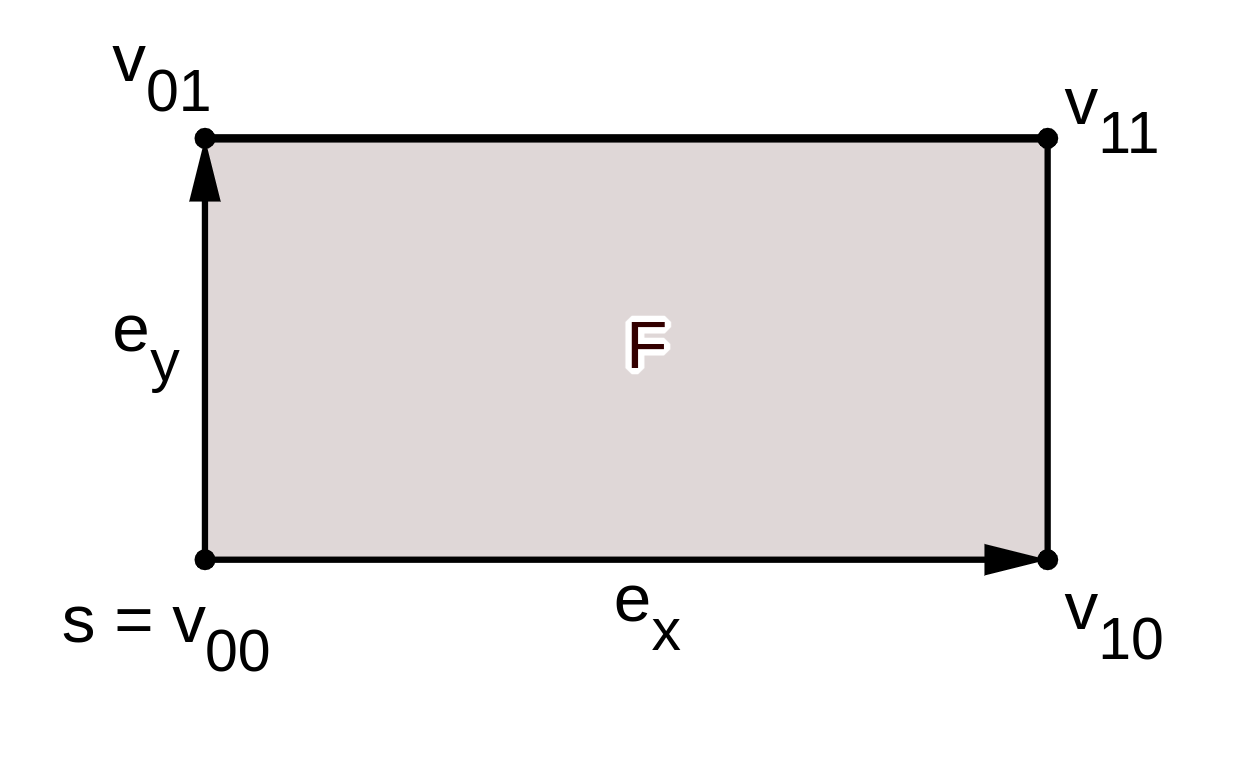
\includegraphics[width=0.6\textwidth]{imagenes/figura4_1}
  \end{minipage}}
  \fbox{\begin{minipage}{\dimexpr \textwidth-2\fboxsep-2\fboxrule}
    \abovecaptionskip=0pt
    \caption{Puntos relevantes de la fuente de luz rectangular $F$.}
  \end{minipage}}
\end{figure}

\subsection{Construcción de la parametrización $M$ }

En primer lugar, describiremos el sistema de referencia en el que vamos a trabajar. Fijemos $P\in\mathds{R}^3$ el punto desde el cual queremos muestrear el ángulo sólido subtendido por el rectángulo $F$. Fijemos un vértice $s$ del rectángulo $F$ y consideremos los dos vectores $e_x$ y $e_y$ cuyo punto inicial es el vértice $s$ y cuyos puntos finales son los vértices adyacentes a $s$ (véase la figura 5.1). Sea $z$ el vector de longitud unidad perpendicular a $e_x$ y $e_y$ tal que $(s-P)\cdot z < 0$. Entonces, notando $x=\frac{e_x}{\|e_x\|}$, $y=\frac{e_y}{\|e_y\|}$, trabajaremos respecto al sistema de referencia $S=\{P; (x, y, z)\}$, por lo que todos los vectores de coordenadas serán respecto a $S$.

Consideramos ahora los siguientes valores:
$$ x_0 = (s-P)\cdot x\hspace{0.5cm}y_0 = (s-P)\cdot y\hspace{0.5cm}z_0 = (s-P)\cdot z$$
$$\hspace{0.5cm}x_1 = x_0+\|e_x\|\hspace{0.5cm}y_1 = y_0+\|e_y\|$$

Notaremos $v_{ij} := (x_i,y_j,z_0)$, $i=0,1$, $j=0,1$, a los cuatro vértices del rectángulo $F$. Consideramos la pirámide con ápide $P$ y base $F$, y tomamos las normales a cada uno de los planos laterales de la pirámide:
$$ n_0 = \frac{v_{00}\times v_{10}}{\|v_{00}\times v_{10}\|}\hspace{0.5cm}n_1 = \frac{v_{10}\times v_{11}}{\|v_{10}\times v_{11}\|}$$
$$ n_2 = \frac{v_{11}\times v_{01}}{\|v_{11}\times v_{01}\|}\hspace{0.5cm}n_3 = \frac{v_{01}\times v_{00}}{\|v_{01}\times v_{00}\|}$$

Notamos por $\gamma_i := \arccos(-n_i\cdot n_{i+1})$, $i=0,1,2$, $\gamma_3 := \arccos(-n_3\cdot n_0)$ al ángulo interior que forman los planos laterales de la pirámide. Se puede demostrar utilizando el teorema de Girard que el ángulo sólido subtendido por $F$ desde $P$ o, equivalentemente, el área de $\pi_P(F)$, mide:
$$\mu(\pi_P(F)) = \gamma_0 +\gamma_1 + \gamma_2 + \gamma_3 - 2\pi $$

Dado que $F$, que es la base de la pirámide descrita, tiene los lados paralelos a los ejes de coordenadas, se cumple que $n_i$ tendrá al menos una coordenada nula para todo $i$. En efecto vemos que existen $\varphi_0,\ldots,\varphi_3$ tales que:
$$ n_0 = \cos(\varphi_0)z + \sin(\varphi_0)y\hspace{0.5cm}n_1 = \cos(\varphi_1)z + \sin(\varphi_1)x$$
$$ n_2 = \cos(\varphi_2)z + \sin(\varphi_2)y\hspace{0.5cm}n_3 = -\cos(\varphi_3)z - \sin(\varphi_3)x$$

Pasamos ya a construir la parametrización $M$ que preserva el área. Tomamos $v=(v_1,v_2)\in [0,1]^2$. Pretendemos encontrar $(x_v,y_v,z_0)$ las coordenadas respecto al sistema de referencia $S$ de un punto en $F$ tal que su proyección sobre la esfera sea igual a $M(v)$. Para calcular $x_v$, establecemos un rectángulo esférico $Q_v$ contenido en $\pi_P(F)$ tal que el área de $Q_v$ cumpla que:
$$\mu(Q_v) = \mu(\pi_P(F)) v_1 $$

Para que $M$ preserve el área tendremos que el rectángulo esférico $Q_v$ es el resultante de proyectar sobre la esfera la parte del rectángulo $F$ que cumple que su primera coordenada es menor o igual que $x_v$. 

\begin{figure}[h]
  \lineskip=-\fboxrule
  \fbox{\begin{minipage}{\dimexpr \textwidth-2\fboxsep-2\fboxrule}
    \centering
    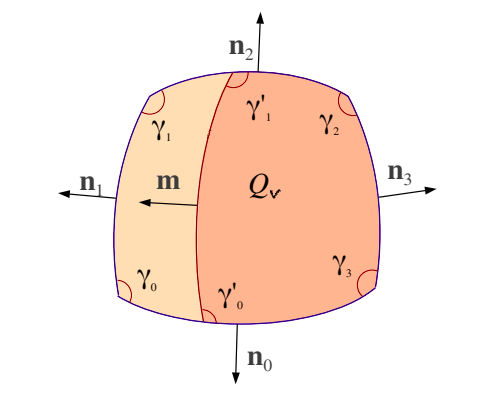
\includegraphics[width=0.6\textwidth]{imagenes/figura4_2}
  \end{minipage}}
  \fbox{\begin{minipage}{\dimexpr \textwidth-2\fboxsep-2\fboxrule}
    \abovecaptionskip=0pt
    \caption{Descripción de los rectángulos esféricos $\pi_P(F)$ y $Q_v$}
    \source{\cite{Urena2013}}
  \end{minipage}}
\end{figure}

Como podemos ver en la figura 5.2, tres de los cuatro planos que delimitan el rectángulo $\pi_P(F)$ también delimitan $Q_v$. El cuarto plano delimitante es el plano que pasa por $P$ y que es perpendicular a cierto vector $m$ perteneciente al plano $y=0$. Por tanto, para algún $\varphi_v$ se tiene que:
$$m=\cos(\varphi_v)z+\sin(\varphi_v)x$$

El ángulo $\varphi_v$ sólo dependerá de $v_1$ y varía desde $\varphi_3$ hasta $\varphi_1$. El área de $Q_v$ cumple que:
\begin{align*}
\mu&(\pi_P(F))v_1 = \mu(Q_v) = \arccos(-n_0\cdot m) +\arccos(-m\cdot n_2) + \gamma_2 +\gamma_3 -2\pi =\\
&= \arccos(-\cos(\varphi_0) \cos(\varphi_v)) +\arccos(-\cos(\varphi_2) \cos(\varphi_v)) + \gamma_2 +\gamma_3 -2\pi 
\end{align*}

Utilizando esta última igualdad y haciendo una serie de derivaciones (ver \cite{Urena2013}) obtenemos que:
$$\cos(\varphi_v) = \frac{\text{sign}(g(v_1))}{\sqrt{g(v_1)^2+\cos(\varphi_0)}}, $$
$$g(v_1) = \frac{\cos(\Phi(v_1))\cos(\varphi_0) - \cos(\varphi_2)}{\sin(\Phi(v_1))}, $$
$$\Phi(v_1) = v_1\mu(\pi_P(F))-\gamma_2-\gamma_3+2\pi$$


\begin{figure}[h]
  \lineskip=-\fboxrule
  \fbox{\begin{minipage}{\dimexpr \textwidth-2\fboxsep-2\fboxrule}
    \centering
    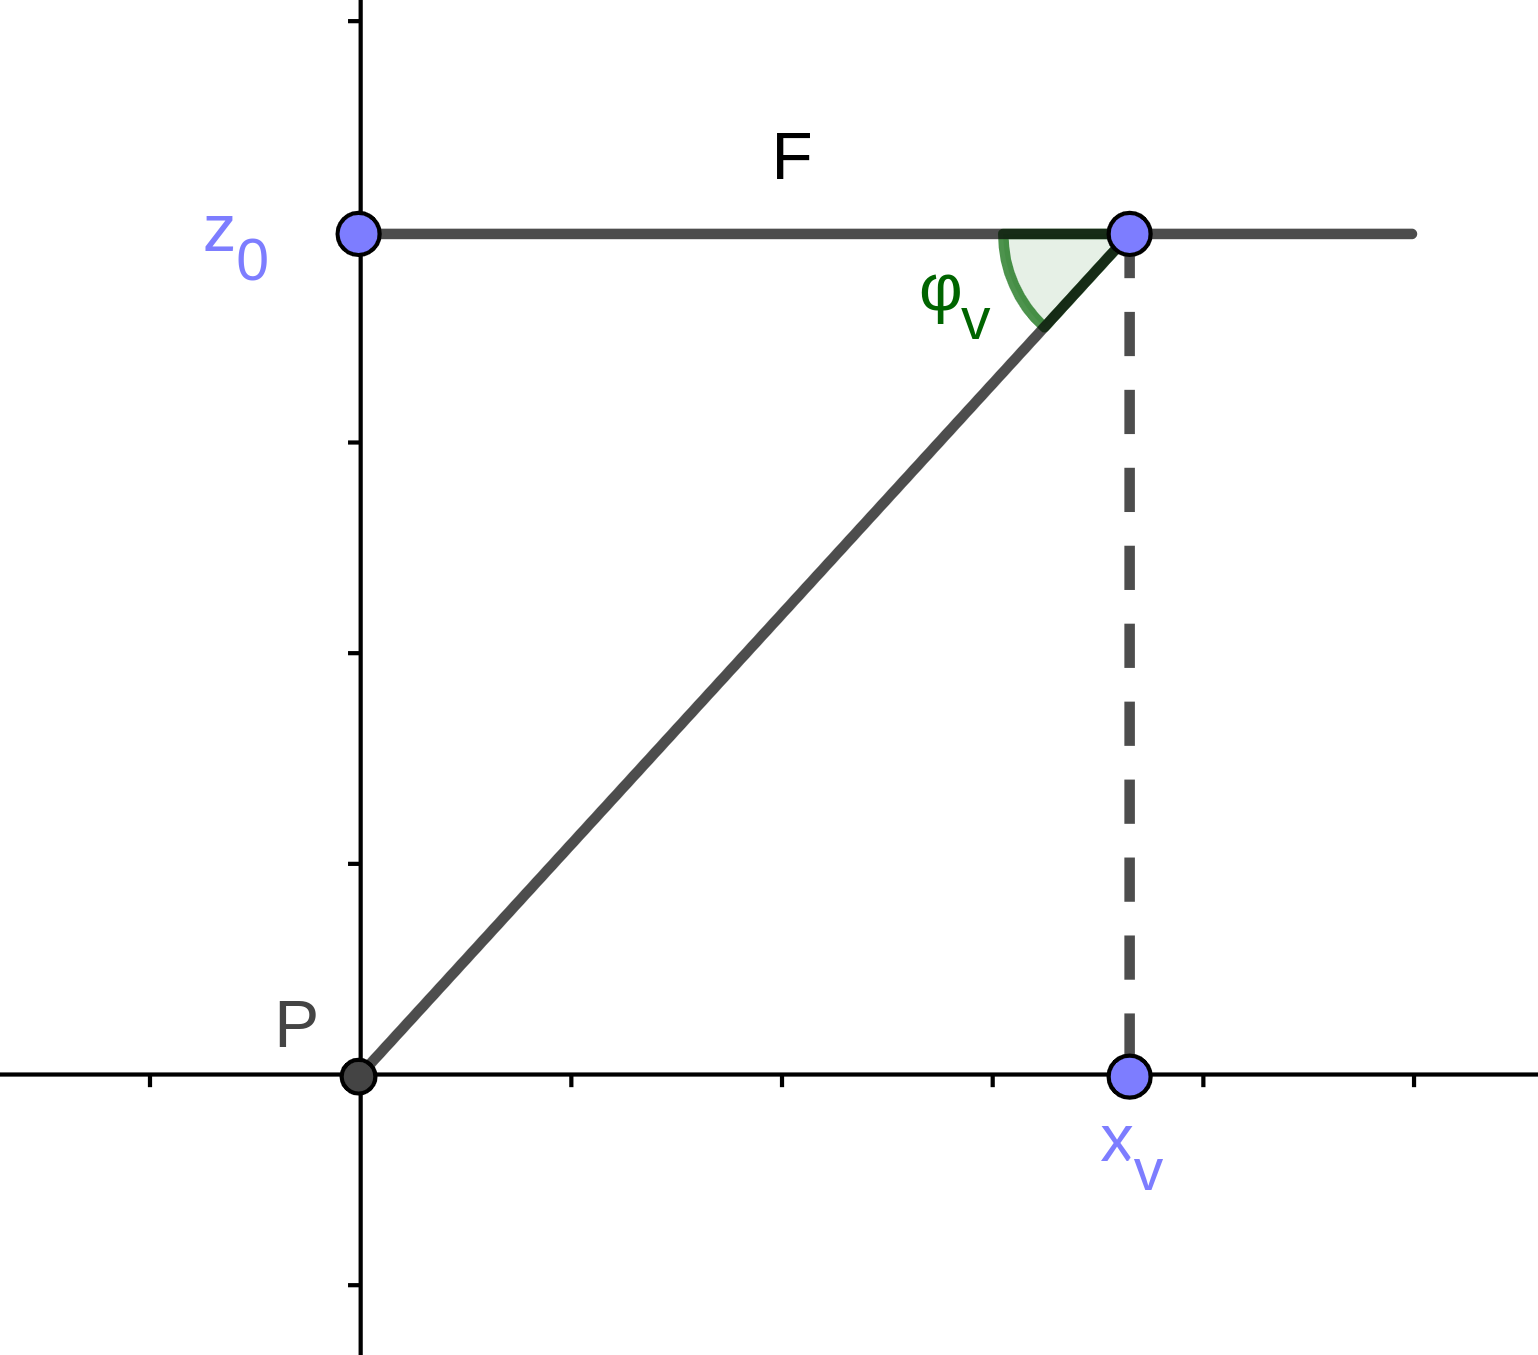
\includegraphics[width=0.6\textwidth]{imagenes/figura4_3}
  \end{minipage}}
  \fbox{\begin{minipage}{\dimexpr \textwidth-2\fboxsep-2\fboxrule}
    \abovecaptionskip=0pt
    \caption{Relación entre $x_v$ y $\varphi_v$}
  \end{minipage}}
\end{figure}

En vista de la figura 5.3, podemos obtener $x_v$ de manera sencilla a partir de $\cos(\varphi_v)$:
$$x_v = -\cos(\varphi_v)\frac{z_0}{\sin(\varphi_v)} = -\cos(\varphi_v)\frac{z_0}{\sqrt{1-\cos(\varphi_v)^2}} $$

Por último, calculemos $y_v$. Ya sabemos que la proyección de $M(v)$ sobre $F$ estará en el segmento:
$$\{(x_v, t y_1 + (1-t) y_0, z_0) / t\in [0,1]\}$$

Para que $M$ preserve el área, en vista de la igualdad \ref{intAngSolSin}, se tiene que cumplir que cambios iguales en $v_2$ generen cambios iguales en $\sin(\theta)$, con $\theta$ el ángulo entre los vectores $y$ y $M(v)$. Para ello, podemos interpolar linealmente la segunda componente de $M(v)$, $h_v$, de la siguiente manera:
$$h_v = h_0 + v_2(h_1-h_0) $$
$$h_0=\frac{y_0}{\sqrt{x_v^2+z_0^2+y_0^2}} $$
$$h_1=\frac{y_1}{\sqrt{x_v^2+z_0^2+y_1^2}}$$

Y concluimos que:
$$y_v = \frac{h_v \sqrt{x_v^2+z_0^2}}{\sqrt{1-h_v^2}}$$

Para finalizar, podemos normalizar el vector $(x_v, y_v, z_0)$, tomando:
$$(\overset{\wedge}{x_v}, h_v, \overset{\wedge}{z_0}) = (x_v, y_v, z_0)\frac{1}{\sqrt{x_v^2 + y_v^2 + z_0^2}}$$

Y tenemos que la dirección $M(v)$ respecto al sistema de referencia usual cumple:
$$M(v) = \overset{\wedge}{x_v} \cdot x + h_v\cdot y + \overset{\wedge}{z_0}\cdot z $$

\subsection{Resultados obtenidos}

Este algoritmo ha sido implementado en \cite{pbrtCode}. Como vemos en la figura 5.4, con una fuente de luz pequeña ya se aprecia una importante mejora empleando el muestreo uniforme respecto al ángulo sólido en comparación al método de muestreo clásico que usa una función de densidad uniforme respecto al área de la fuente de luz. Destacar que todas las imágenes mostradas en este apartado han sido generadas aplicando muestreo de importancia múltiple, combinando así el muestreo de las fuentes de luz y de la función de distribución de dispersión, BSDF.

\begin{figure}[h]
  \lineskip=-\fboxrule
  \fbox{\begin{minipage}{\dimexpr .5\textwidth-\fboxsep-2\fboxrule}
    \begin{subfigure}{\textwidth}
            \centering
            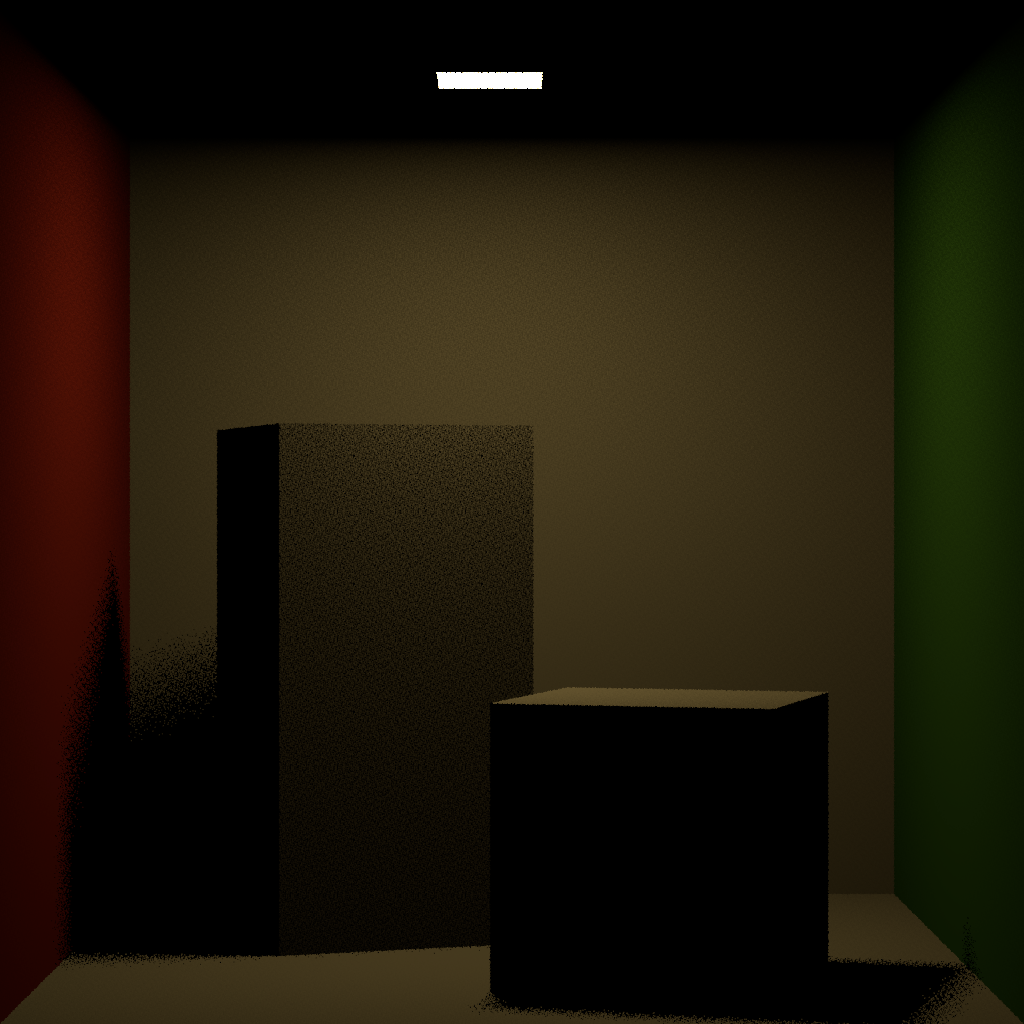
\includegraphics[width=\textwidth]{imagenes/rect1}
            %\caption{Rectángulo esférico}
            %\end{subfigure}
            %\begin{subfigure}{\textwidth}
            %\centering
            \vspace{0.2cm}
            
            
\includegraphics[width=\textwidth]{imagenes/rect12}
            \caption{Uniforme respecto al área}
            \end{subfigure}  
    \end{minipage}
    \hfill
\begin{minipage}{\dimexpr .5\textwidth-\fboxsep-2\fboxrule}
   \begin{subfigure}{\textwidth}
            \centering
            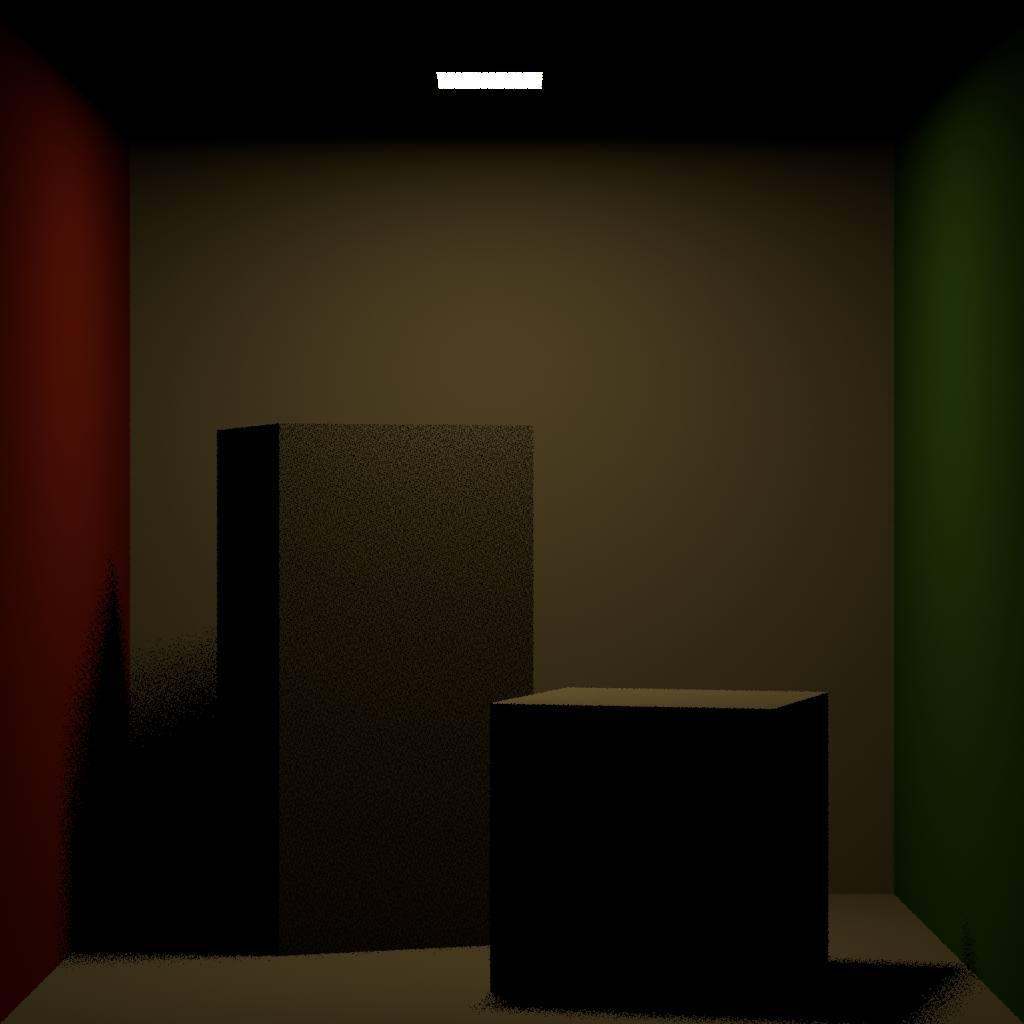
\includegraphics[width=\textwidth]{imagenes/rect2}
            \vspace{0.2cm}

            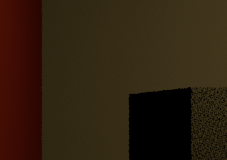
\includegraphics[width=\textwidth]{imagenes/rect21}
            \caption{Rectángulo esférico}
            \end{subfigure}% 
  \end{minipage}}
  \fbox{\begin{minipage}{\dimexpr \textwidth-\fboxsep-2\fboxrule}
    \abovecaptionskip=0pt
    \caption{Comparativa entre muestreo uniforme respecto al área y muestreo uniforme respecto al ángulo sólido. Imágenes con una muestra por píxel y con el algoritmo de iluminación directa.}
  \end{minipage}}
\end{figure}

Si usamos una fuente de luz de mayor tamaño, la reducción de la varianza se aprecia más claramente (ver figura 5.5).   

\begin{figure}[h!]
  \lineskip=-\fboxrule
  \fbox{\begin{minipage}{\dimexpr .5\textwidth-\fboxsep-2\fboxrule}
    \begin{subfigure}{\textwidth}
            \centering
            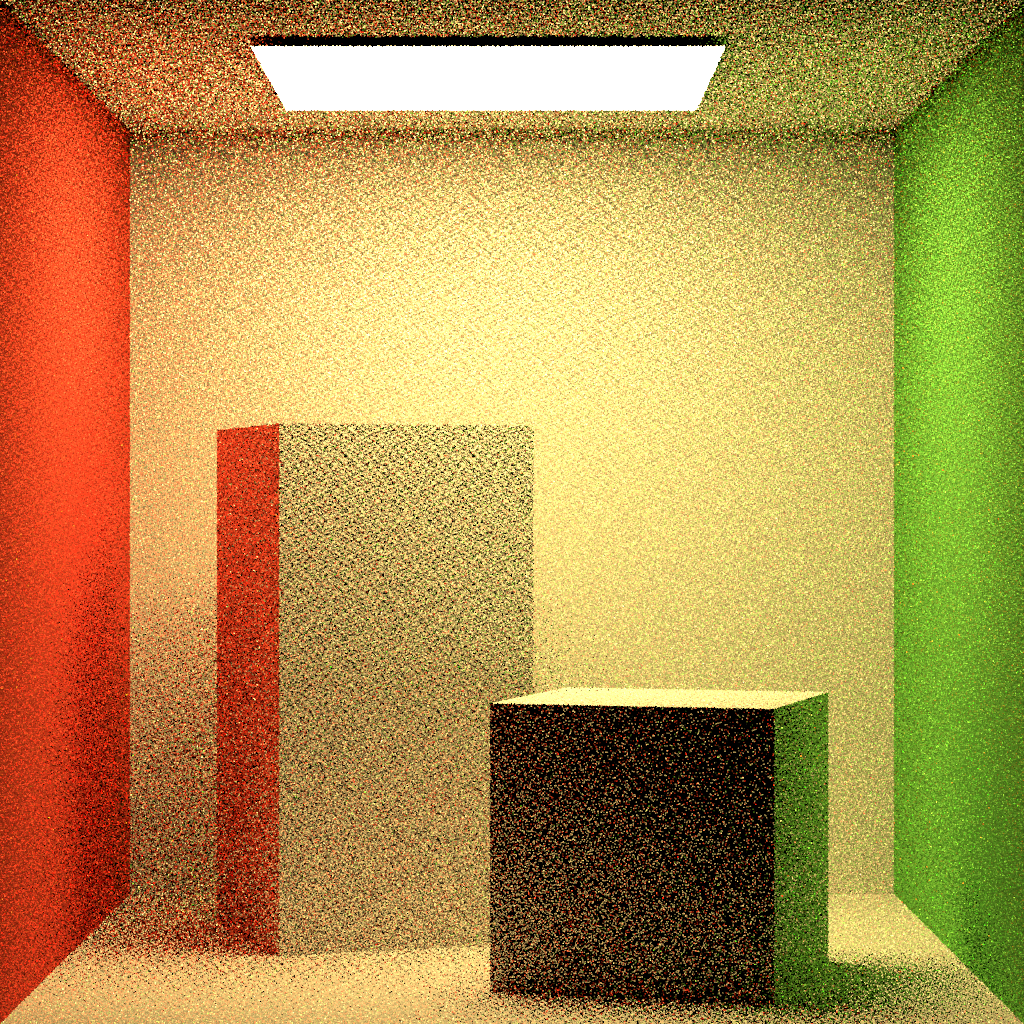
\includegraphics[width=\textwidth]{imagenes/rectangle5}
            \caption{Path tracing, área}
            \end{subfigure}
            \begin{subfigure}{\textwidth}
            \centering
            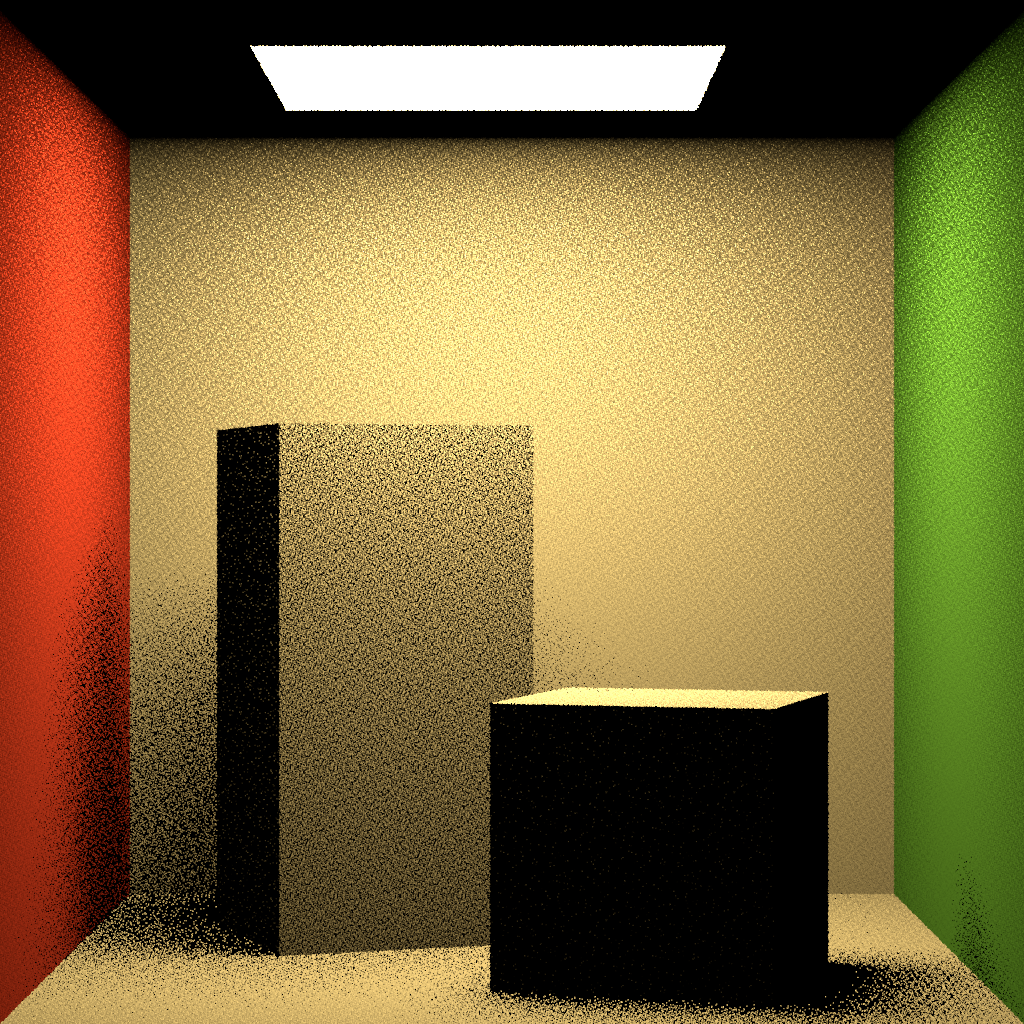
\includegraphics[width=\textwidth]{imagenes/rectangle7}
            \caption{Iluminación directa, área}
            \end{subfigure}  
    \end{minipage}
    \hfill
\begin{minipage}{\dimexpr .5\textwidth-\fboxsep-2\fboxrule}
   \begin{subfigure}{\textwidth}
            \centering
            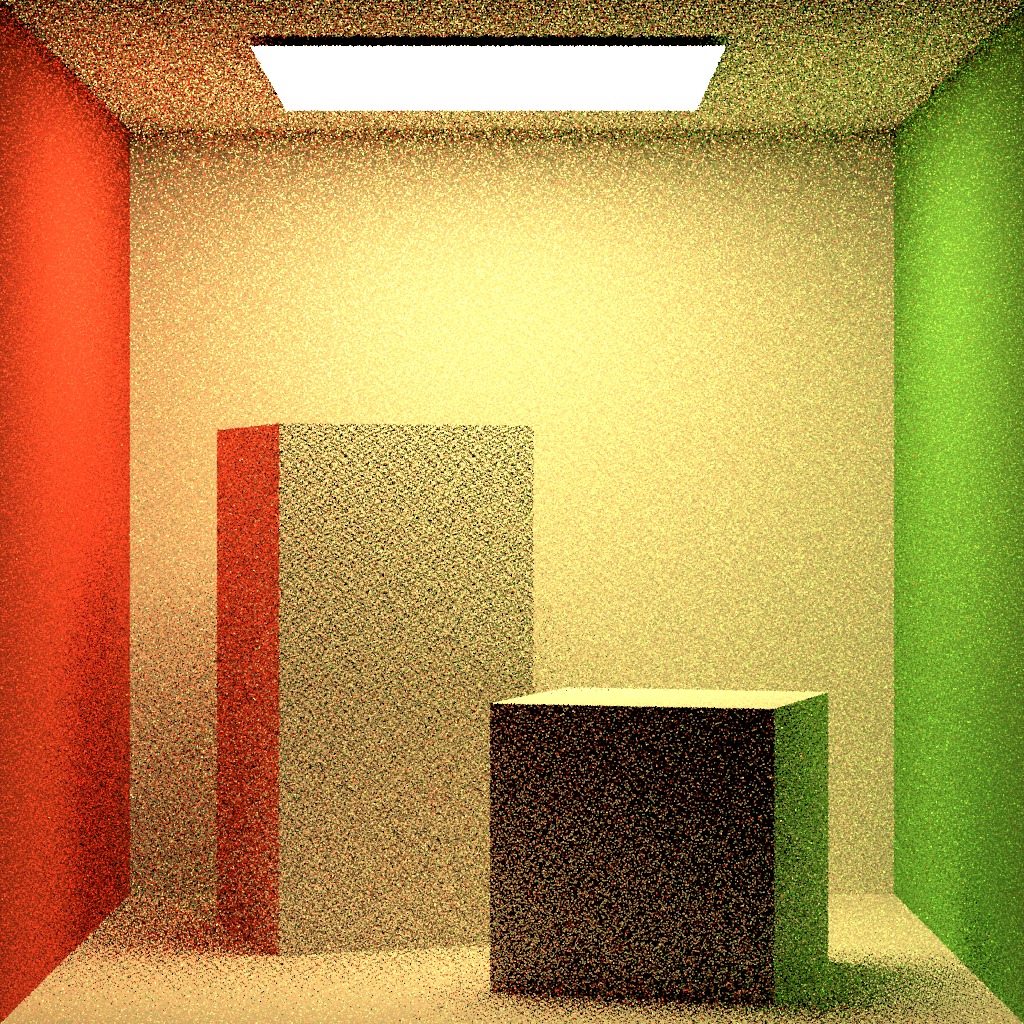
\includegraphics[width=\textwidth]{imagenes/rectangle6}
            \caption{Path tracing, ángulo sólido}
            \end{subfigure}
            \begin{subfigure}{\textwidth}
            \centering
            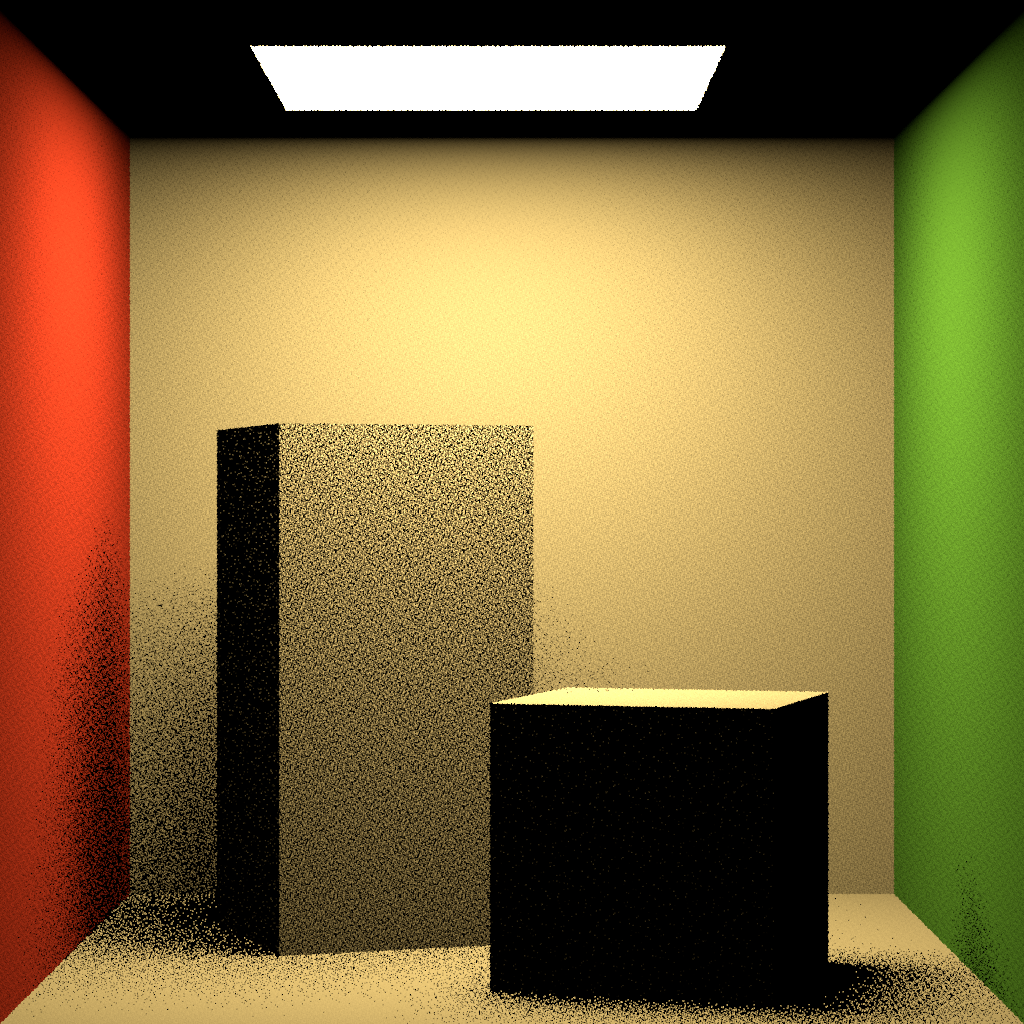
\includegraphics[width=\textwidth]{imagenes/rectangle8}
            \caption{Iluminación directa, ángulo sólido}
            \end{subfigure}% 
  \end{minipage}}
  \fbox{\begin{minipage}{\dimexpr \textwidth-\fboxsep-2\fboxrule}
    \abovecaptionskip=0pt
    \caption{Comparativa entre muestreo uniforme respecto al área y muestreo uniforme respecto al ángulo sólido. Imágenes generadas con una muestra por píxel.}
  \end{minipage}}
\end{figure}

\newpage
Por otra parte, este algoritmo implica un aumento en el tiempo de ejecución, ya que la cantidad de operaciones y su complejidad es mucho mayor que en el caso del muestreo uniforme respecto al área. Sin embargo, como podemos observar en la figura 5.6, si generamos la imagen con dos muestras por píxel usando el muestreo uniforme respecto al área, el tiempo de ejecución es mayor que en el caso de una muestra por píxel utilizando el algoritmo descrito, pero en las superficies desde las que es completamente visible la fuente de luz sigue teniendo mejores resultados el muestreo del rectángulo esférico.

\begin{figure}[h!]
  \lineskip=-\fboxrule
  \fbox{\begin{minipage}{\dimexpr .5\textwidth-\fboxsep-2\fboxrule}
    \begin{subfigure}{\textwidth}
            \centering
            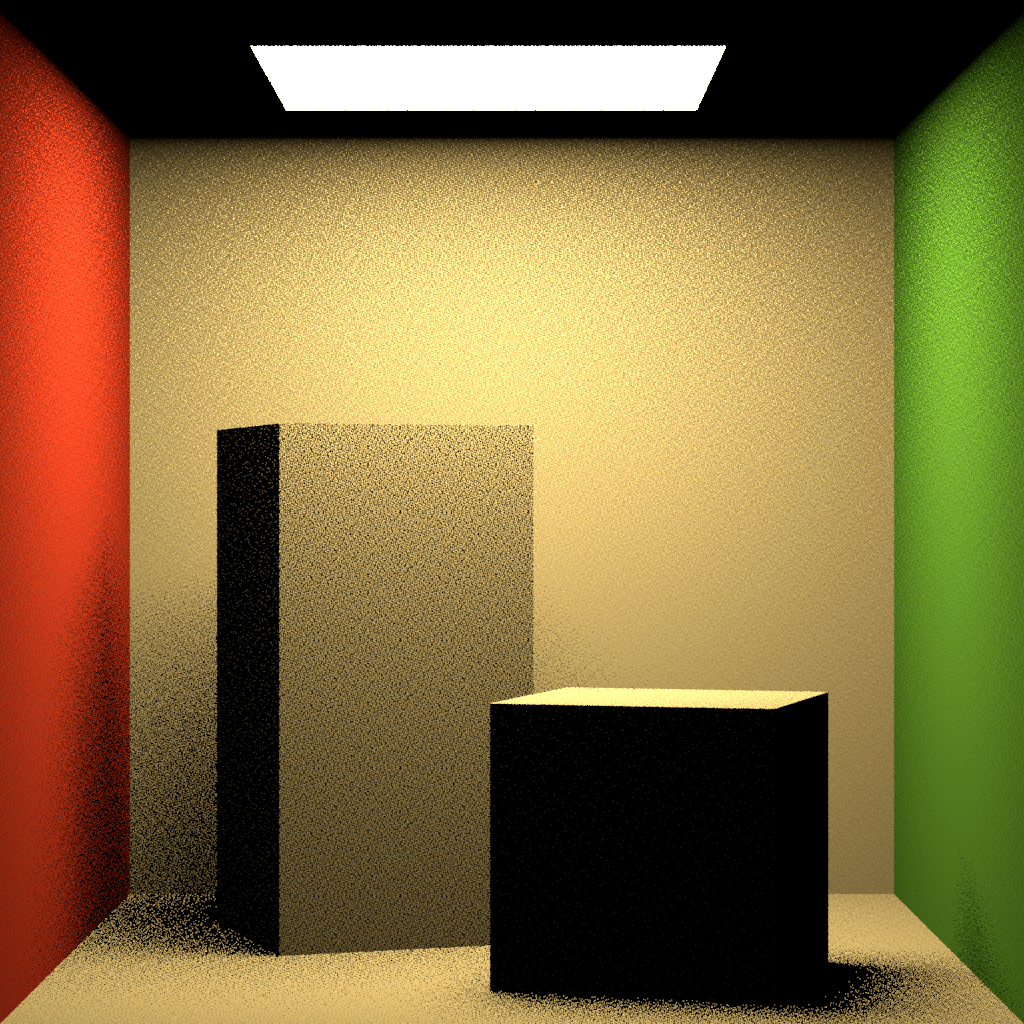
\includegraphics[width=\textwidth]{imagenes/rectangle11}
            \caption{2 muestras pp, área, 2.642 seg}
            \end{subfigure} 
    \end{minipage}
    \hfill
    \begin{minipage}{\dimexpr .5\textwidth-\fboxsep-2\fboxrule}
            \begin{subfigure}{\textwidth}
            \centering
            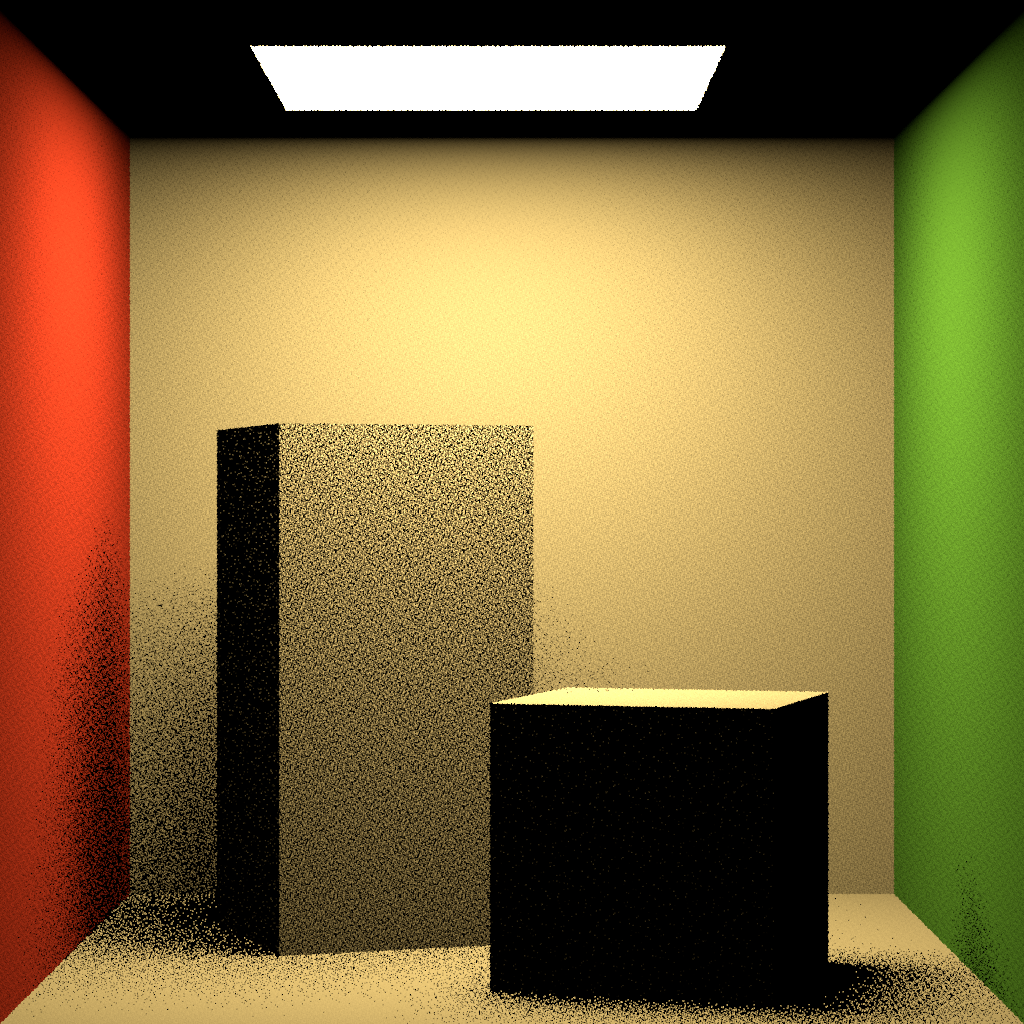
\includegraphics[width=\textwidth]{imagenes/rectangle8}
            \caption{1 muestra pp, ángulo sólido, 1.654 seg}
            \end{subfigure}  
    \end{minipage}}
  \fbox{\begin{minipage}{\dimexpr \textwidth-\fboxsep-2\fboxrule}
    \abovecaptionskip=0pt
    \caption{Comparativa entre muestreo uniforme respecto al área y muestreo uniforme respecto al ángulo sólido.}
  \end{minipage}}
\end{figure}

Por último, en la figura 5.7 vemos una comparativa de tiempo entre los dos algoritmos para generar la imagen de la caja de Cornell, tanto para iluminación directa como para path-tracing.

\begin{figure}[h!]
  \lineskip=-\fboxrule
  \fbox{\begin{minipage}{\dimexpr .5\textwidth-\fboxsep-2\fboxrule}
    \begin{subfigure}{\textwidth}
            \centering
            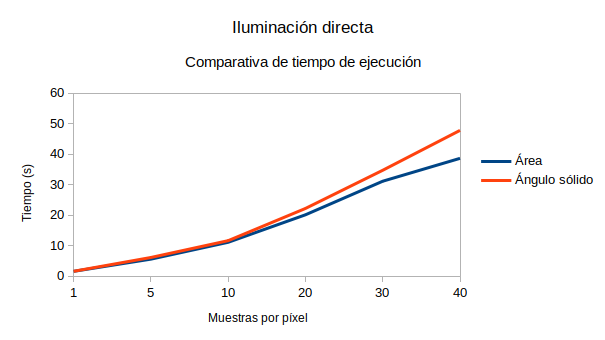
\includegraphics[width=\textwidth]{imagenes/compdl}
            \caption{Iluminación Global}
            \end{subfigure} 
    \end{minipage}
    \hfill
    \begin{minipage}{\dimexpr .5\textwidth-\fboxsep-2\fboxrule}
            \begin{subfigure}{\textwidth}
            \centering
            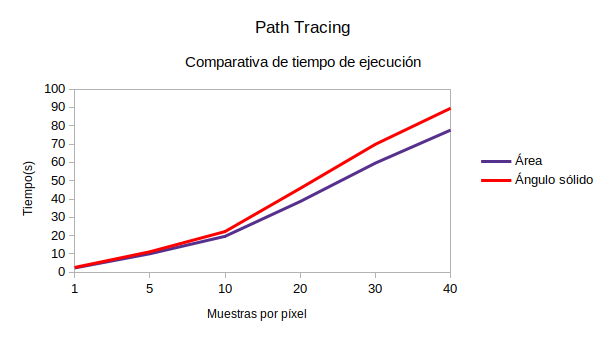
\includegraphics[width=\textwidth]{imagenes/comppath}
            \caption{Path-tracing}
            \end{subfigure}  
    \end{minipage}}
  \fbox{\begin{minipage}{\dimexpr \textwidth-\fboxsep-2\fboxrule}
    \abovecaptionskip=0pt
    \caption{Comparativa del tiempo de ejecución.}
  \end{minipage}}
\end{figure}

Concluimos que, aunque este algoritmo incremente el tiempo de ejecución, reduce significativamente la varianza del estimador de la radiancia, especialmente en las superficies desde las que la fuente de luz es completamente visible y cuando la superficie de la fuente de luz es grande respecto a las dimensiones de la escena renderizada. 
 

\section{Muestreo uniforme de elipses esféricas}

Procedemos de manera similar al caso de fuentes de luz rectangulares. El algoritmo descrito a continuación está recogido en \cite{Guillen2017}. Una elipse esférica es la proyección sobre la esfera unidad de un disco. Consideramos una fuente de luz $D$ cuya superficie es un disco, y fijamos un punto $o\in\mathds{R}^3$ respecto al cual queremos muestrear las direcciones contenidas en la elipse esférica $\pi_o(D)$ siguiendo una distribución uniforme. En este caso construiremos dos parametrizaciones, $M_r:[0,1]^2\rightarrow \pi_o(D)$, $M_s:[0,1]^2\rightarrow \pi_o(D)$, que preservan el área.

\begin{figure}[h]
  \lineskip=-\fboxrule
  \fbox{\begin{minipage}{\dimexpr \textwidth-2\fboxsep-2\fboxrule}
    \centering
    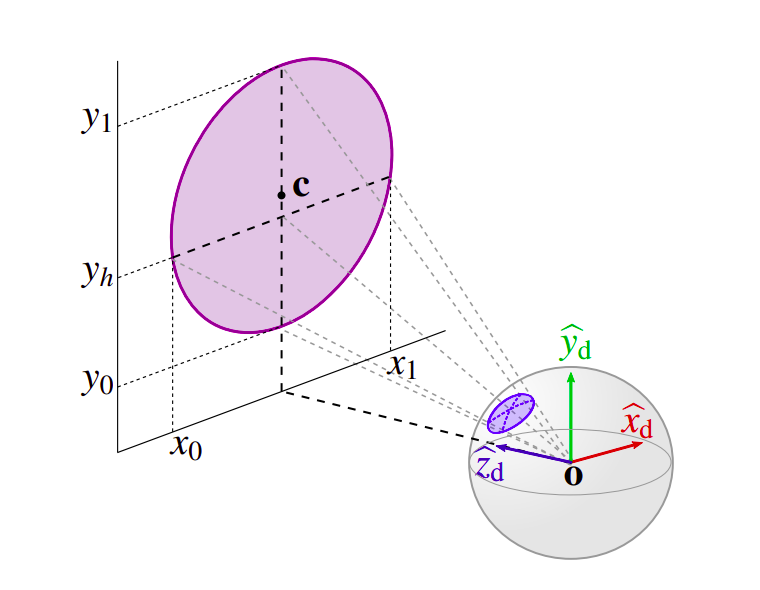
\includegraphics[width=0.6\textwidth]{imagenes/figura4_4}
  \end{minipage}}
  \fbox{\begin{minipage}{\dimexpr \textwidth-2\fboxsep-2\fboxrule}
    \abovecaptionskip=0pt
    \caption{Sistema de referencia y puntos relevantes}
    \source{\cite{Guillen2017}}
  \end{minipage}}
\end{figure}

\subsection{Descripción del sistema de referencia y otros parámetros}

Dada $n_D$ la normal al disco $D$, $c$ el centro del disco $D$, y consideremos los tres siguientes vectores:
$$z_d = -n_D $$
$$x_e = z_d\times \frac{c-P}{\|c-P\|} $$
$$y_d = x_e\times z_d $$

Tomamos el sistema de referencia $S_1=\{o;(x_e, y_d, z_d)\}$ (ver figura 5.8) y todos los vectores de coordenadas aquí descritos serán respecto a $S_1$. Consideramos los puntos $y_0$ e $y_1$ donde el disco toma el valor mínimo y máximo en la segunda coordenada. Si proyectamos $y_0$ e $y_1$ sobre la esfera unidad con centro $o$ obtendremos dos puntos $(0,y_0',z_0')$, $(0,y_1',z_1')$. Entonces el centro de la elipse esférica $\pi_o(D)$ se puede calcular como:
$$z_e = (0,\frac{y_0'+y_1'}{2}, \frac{z_0' + z_1'}{2}) $$

Notar que al reproyectar $z_e$ en el disco obtenemos un punto $(0,y_h,z_h)$ que en general no tiene porque coincidir con el centro del disco $c$. La recta $y = y_h$, $z=z_h$ intersecciona con el disco en dos puntos, $x_0$ y $x_1$. Proyectamos de nuevo el punto $x_1$ sobre la esfera unidad, y consideramos la primera coordenada del punto proyectado, que llamaremos $x_1'$. Por último tomamos los siguientes valores:
\begin{align*}
a = x_1'&\hspace{1cm} b=\frac{1}{2}\sqrt{(y_1'-y_0')^2 + (z_1'-z_0')^2}\\
\alpha = \sin^{-1}(a)&\hspace{1cm} \beta=\sin^{-1}(b)\\
a_t = \tan(\alpha) &\hspace{1cm}b_t=\tan(\beta)
\end{align*}

donde $a$ y $b$ son los semi-ejes de la elipse esférica, $\alpha$ y $\beta$ son sus semi-arcos. Tomando $y_e=z_e\times x_e$, de aquí en adelante cambiaremos el sistema de referencia y trabajaremos sobre $S=\{o;(x_e, y_e, z_e)\}$.

Antes de pasar a describir las dos parametrizaciones, destacar que estas están basadas en el siguiente resultado:

\begin{proposicion}
Sea $\mathds{S}^2$ la esfera unidad de $\mathds{R}^3$, y sea $C$ el cilindro de radio unidad cuyo eje está alineado con el eje $X$. Consideremos la transformación:
$$T:\mathds{S}^2/\{(0,0,1),(0,0,-1)\}\rightarrow C, \hspace{0.7cm} T(x,y,z) = (\frac{x}{\sqrt{x^2+y^2}}, \frac{y}{\sqrt{x^2+y^2}}, z)$$

Entonces dado $A\subseteq\mathds{S}^2$ se cumple que:
$$\int_A dS = \int_{T(A)} dS$$
\end{proposicion}
\begin{proof}
Consideramos la parametrización $\Theta:[0,\pi ]\times [0,2\pi ]\rightarrow \mathds{S}^2$, con:
$$\Theta(\theta ,\varphi ) = ( \sin \theta \cos \varphi,  \sin \theta \sin \varphi , \cos \theta),\hspace{0.5cm}  \forall (\theta , \varphi)\in [0,\pi ]\times [0,2\pi ]$$

Consideramos también la parametrización $\Psi:[0,2\pi ]\times [-1,1]\rightarrow C$, con:
$$\Psi(\varphi , z ) = (\cos \varphi,  \sin \varphi , z),\hspace{0.5cm}  \forall (\varphi, z)\in [0,2\pi ]\times [-1,1]$$

Por la igualdad \ref{intAngSolSin}, y haciendo un sencillo cálculo, vemos que:
$$\int_A dS = \int_{\Theta^{-1}(A)} \sin\theta d\theta d\varphi$$
$$\int_{T(A)} dS = \int_{\Psi^{-1}(T(A))} d\varphi dz $$

Consideramos la función:
$$R:[0,\pi]\times [0,2\pi]\rightarrow [0,2\pi]\times [-1,1] \text{, } R(\theta,\varphi) = (\varphi, \cos(\theta))$$

que cumple que $|det(J_R(\theta,\varphi))| = \sin(\theta)$. Por tanto, aplicando el teorema de cambio de variable, basta ver que $R(\Theta^{-1}(A)) = \Psi^{-1}(T(A))$ para deducir el resultado buscado, lo cuál se deduce fácilmente.
\end{proof}

Este resultado nos dice que el ángulo sólido subtendido por una región de la esfera unidad es igual que el área de esa región proyectada sobre el cilindro de radio uno tal que su eje está alineado con un radio de la esfera.

\subsection{Construcción de la parametrización $M_r$}
Partimos de una muestra $v=(v_1,v_2)\in[0,1]^2$, y vamos a describir como se obtiene la dirección $M_r(v)$ a partir de $v$. En este caso consideramos el cilindro de radio unidad cuyo eje está alineado con $z_e$. Nos centraremos sólo en el caso de muestrear el primer cuadrante de la elipse, haciendo uso del hecho de que la elipse es radialmente simétrica. Para muestrear la elipse completa, basta dividir $[0,1]$ en cuatro intervalos, un intervalo por cada cuadrante, y cambiar el sentido de $x_e$ o $y_e$ convenientemente en función del intervalo al que pertenece $v_1$. Tras hacer esto hay que transformar $v_1$ de manera que el intervalo al que pertenece cubra todo $[0,1]$.

\begin{figure}[h]
  \lineskip=-\fboxrule
  \fbox{\begin{minipage}{\dimexpr \textwidth-2\fboxsep-2\fboxrule}
    \centering
    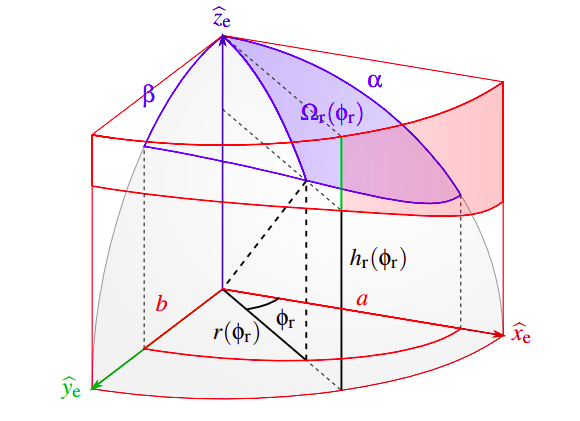
\includegraphics[width=0.6\textwidth]{imagenes/figura4_5}
  \end{minipage}}
  \fbox{\begin{minipage}{\dimexpr \textwidth-2\fboxsep-2\fboxrule}
    \abovecaptionskip=0pt
    \caption{Descripción del mapa $M_r$.}
    \source{\cite{Guillen2017}}
  \end{minipage}}
\end{figure}

Observando la figura 5.9, consideramos la función $\Omega_r:[0,\pi /2]\rightarrow \mathds{R}_0^+$ que a cada ángulo $\phi_r$ respecto al eje $x_e$ le asigna el ángulo sólido subtendido por la región azul de la elipse, o lo que es lo mismo, el área de la región roja del cilindro. Está claro que entonces $\mu(\pi_o(D)) = 4\Omega_r(\frac{\pi}{2})$. Es sencillo ver que:
$$\Omega_r(\phi_r)=\int_0^{\phi_r}[1-h_r(x)] dx$$

donde $h_r$ es la función que asigna a cada ángulo $\phi$ respecto al eje $x_e$ la componente $z_e$ del punto más bajo de la línea verde que delimita la región roja. Mediante una serie de derivaciones llegamos a:
$$\Omega_r(\phi_r) = \phi_r -\frac{b(1-a^2)}{a\sqrt{1-b^2}}\Pi(n;\varphi_r|m) $$

donde
$$\Pi(n;\varphi_r|m) = \int_{0}^{\varphi_r}\frac{dx}{(1-n\sin^2(x))\sqrt{1-m\sin^2(x)}}$$

es la integral elíptica incompleta de Legendre de tercer tipo y donde
$$n = \frac{a^2-b^2}{a^2(1-b^2)}\hspace{1cm} m=\frac{a^2-b^2}{1-b^2} \hspace{1cm} \varphi_r=\arctan(\frac{a_t}{b_t}\tan(\phi_r))$$

Dado que $\Omega_r$ no se puede invertir analíticamente, podemos utilizar el método de Newton-Raphson para encontrar $\phi_v$ cumpliendo que:
$$\Omega_r(\phi_v)-v_1\Omega_r(\pi/2) = 0 $$

Tomamos ahora $h = (1-v_2)h_r(\phi_v) + v_2$, y podemos definir $M_r(v)$ respecto al sistema de referencia usual como:
$$M_r(v) = \cos(\phi_v)\sqrt{1-h^2}\cdot x_e +\sin(\phi_v)\sqrt{1-h^2}\cdot y_e +h\cdot z_e$$

En efecto, $M_r$ preserva el área.

\subsection{Construcción de la parametrización $M_p$}

\begin{figure}[h]
  \lineskip=-\fboxrule
  \fbox{\begin{minipage}{\dimexpr \textwidth-2\fboxsep-2\fboxrule}
    \centering
    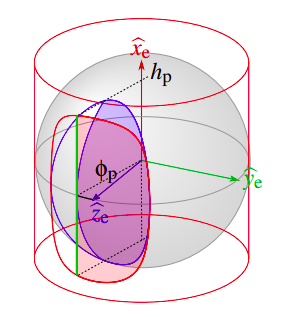
\includegraphics[width=0.5\textwidth]{imagenes/figura4_6}
  \end{minipage}}
  \fbox{\begin{minipage}{\dimexpr \textwidth-2\fboxsep-2\fboxrule}
    \abovecaptionskip=0pt
    \caption{Descripción del mapa $M_p$}
    \source{\cite{Guillen2017}}
  \end{minipage}}
\end{figure}

En este caso, consideramos el cilindro cuyo eje está alineado con el eje $x_e$. En este caso, considerando la imagen 5.10, el ángulo $\phi_p$ va desde $-\beta$ a $\beta$, y la integral del sector cuyo ángulo $\phi_p$ está comprendido entre $-\beta$ y $\phi_p$ (zona roja) se puede calcular como sigue:
$$\Omega_p(\phi_p)=\int_{-\beta}^{\phi_p}2h_p(x)dx,$$

donde $(\phi_p, h_p(\phi_p))$, $(\phi_p, -h_p(\phi_p))$ son los extremos del segmento verde. Claramente el ángulo sólido subtendido por la elipse esférica cumple que:
$$\mu(\pi_o(D)) = \Omega_p(\beta)$$

Se puede derivar una expresión de la función $h_p$, obteniendo (ver \cite{Guillen2017}):
$$h_p(\phi_p)=c_t\sqrt{\frac{1-(p+1)\sin^2\phi_p}{1-(mp+1)\sin^2\phi_p}},$$

donde:
$$p=\frac{1}{b_t^2} \hspace{1cm} m=\frac{a_t^2-b_t^2}{a_t^2+1} \hspace{1cm} c_t=\frac{a_t}{\sqrt{1+a_t^2}}.$$

Claramente por simetría la función $h_p$ cumple que $h_p(x) = h_p(-x)$, $\forall x \in [0,\beta]$. Por tanto, tomando $\Omega_p^+(\phi_p)=\int_0^{\phi_p}2h_p(x)dx$, vemos que:
\[ \Omega_p(\phi_p) =
   \begin{cases}
      \Omega_p^+(\beta)+\Omega_p^+(\phi_p) & :\phi_p\geq0 \\
      \Omega_p^+(\beta)-\Omega_p^+(-\phi_p) & :\phi_p <0
   \end{cases}
  \]

Y sustituyendo la expresión de $h_p$ en $\Omega^+$:
$$\Omega_p^+(\phi_p)=\frac{2c_t}{b_t}[(1-n)\Pi(n;\varphi_p|m)-F(\varphi_p|m)],$$

donde $n=-b_t^2$, $\varphi_p=\sin^{-1}(\frac{\tan\phi_p}{b_t})$, $\Pi$ es la integral elíptica incompleta de Legendre de tercer tipo y $F$ es la integral incompleta de Legendre de primer tipo, es decir:
$$F(\varphi_p | m) = \int_0^{\varphi_p}\frac{dx}{\sqrt{1-m\sin(x)^2}} $$

Procedemos ahora igual que en el apartado anterior. Sea $v=(v_1,v_2)\in[0,1]^2$, utilizamos el algoritmo de Newton-Raphson para encontrar un $\phi_v$ cumpliendo que:
$$\Omega_p(\phi_v)-v_1\Omega_r(\beta) = 0 $$

Tomamos $h = (-1+v_2)h_p(\phi_v) + v_2h_p(\phi_v)$, y podemos definir $M_p(v)$ respecto al sistema de referencia usual como:
$$M_p(v) = h\cdot x_e +\sin(\phi_v)\sqrt{1-h^2}\cdot y_e + \cos(\phi_v)\sqrt{1-h^2}\cdot z_e$$

\subsection{Resultados obtenidos}

Los mapas recién presentados han sido implementados en el renderizador \cite{pbrtCode}, habiéndose utilizado el código de la página \cite{codigoIntegralEliptica} para aproximar el valor de las integrales elípticas. En la figura 5.11 vemos una comparativa entre el muestreo clásico uniforme respecto al área de la fuente de luz y los dos algoritmos aquí presentados. En todas las imágenes aquí mostradas se ha aplicado muestreo de importancia múltiple.

Se puede apreciar que los dos mapas presentados en esta sección reducen la varianza, siendo el mapa paralelo el que mejores resultados ha dado para la escena mostrada. Como vemos, en la superficie de la esfera, que está más alejada de la fuente de luz, la varianza del muestreo uniforme respecto al área se ve reducida, aunque sigue dando mejores resultados el muestreo uniforme respecto al ángulo sólido. En las zonas en las que la fuente de luz es parcialmente visible, el método que peor parece comportarse es el mapa radial.

Por último, en la figura 5.12 vemos una comparativa del tiempo de ejecución de los diferentes métodos. Dado que en los dos métodos expuestos en esta sección se usan aproximaciones de las integrales elípticas, así como inversión numérica de funciones, el tiempo de ejecución es bastante superior al método de muestreo clásico, en especial en el caso del mapa paralelo, en el que se tienen que aproximar dos integrales elípticas cada vez que evaluemos la función $\Omega_p$. Se podría disminuir el tiempo de ejecución de los dos mapas almacenando tablas de valores de las funciones que debemos invertir ($\Omega_p$ y $\Omega_r$), y utilizando dichos valores para aproximar el valor buscado.

\newpage

\begin{figure}[h!]
  \lineskip=-\fboxrule
  \fbox{\begin{minipage}{\dimexpr .33\textwidth-\fboxsep-2\fboxrule}
    \begin{subfigure}{\textwidth}
            \centering
            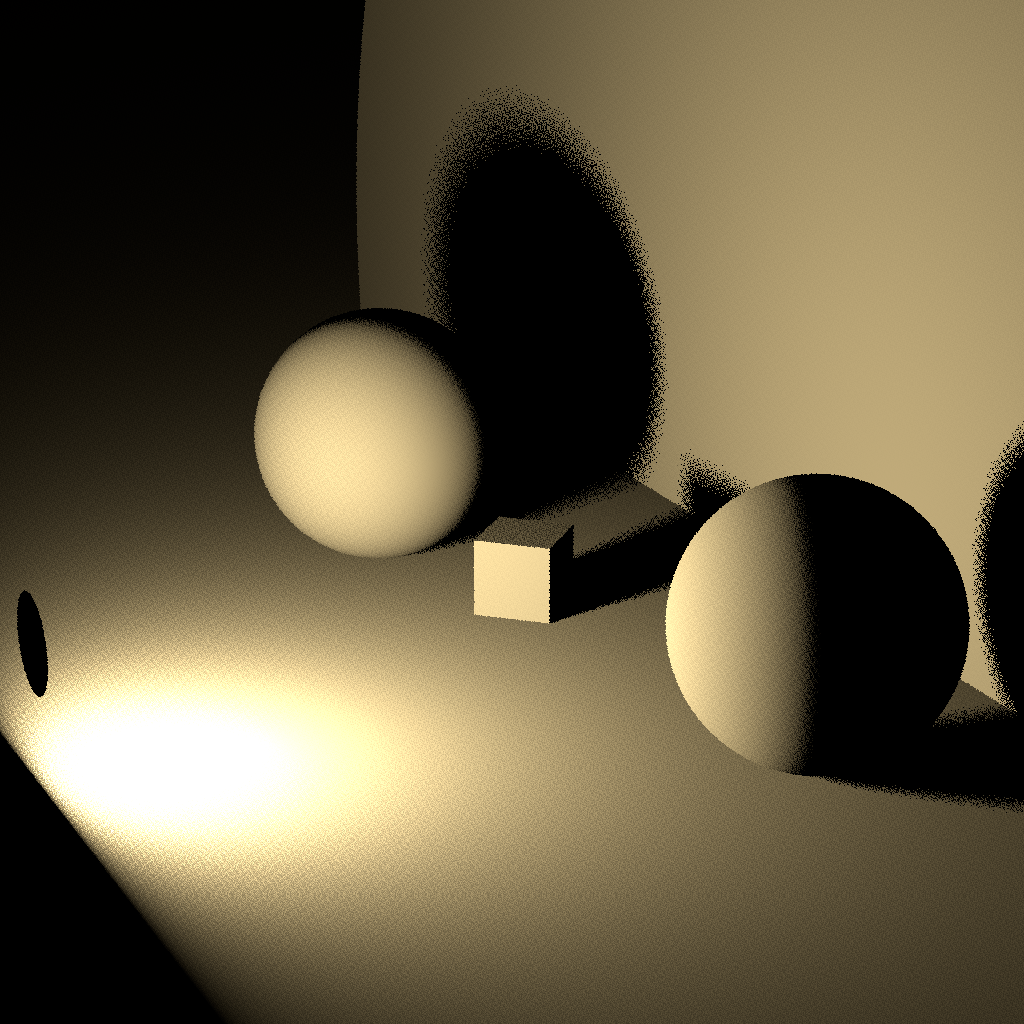
\includegraphics[width=\textwidth]{imagenes/rect8}         
            \vspace{0.2cm}
            
            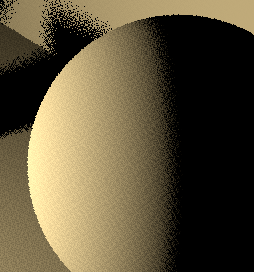
\includegraphics[width=\textwidth]{imagenes/rect81}
            \vspace{0.2cm}

            
\includegraphics[width=\textwidth]{imagenes/rect82}
            \caption{Uniforme área}
            \end{subfigure}  
    \end{minipage}
    \hfill
\begin{minipage}{\dimexpr .33\textwidth-\fboxsep-2\fboxrule}
   \begin{subfigure}{\textwidth}
            \centering
            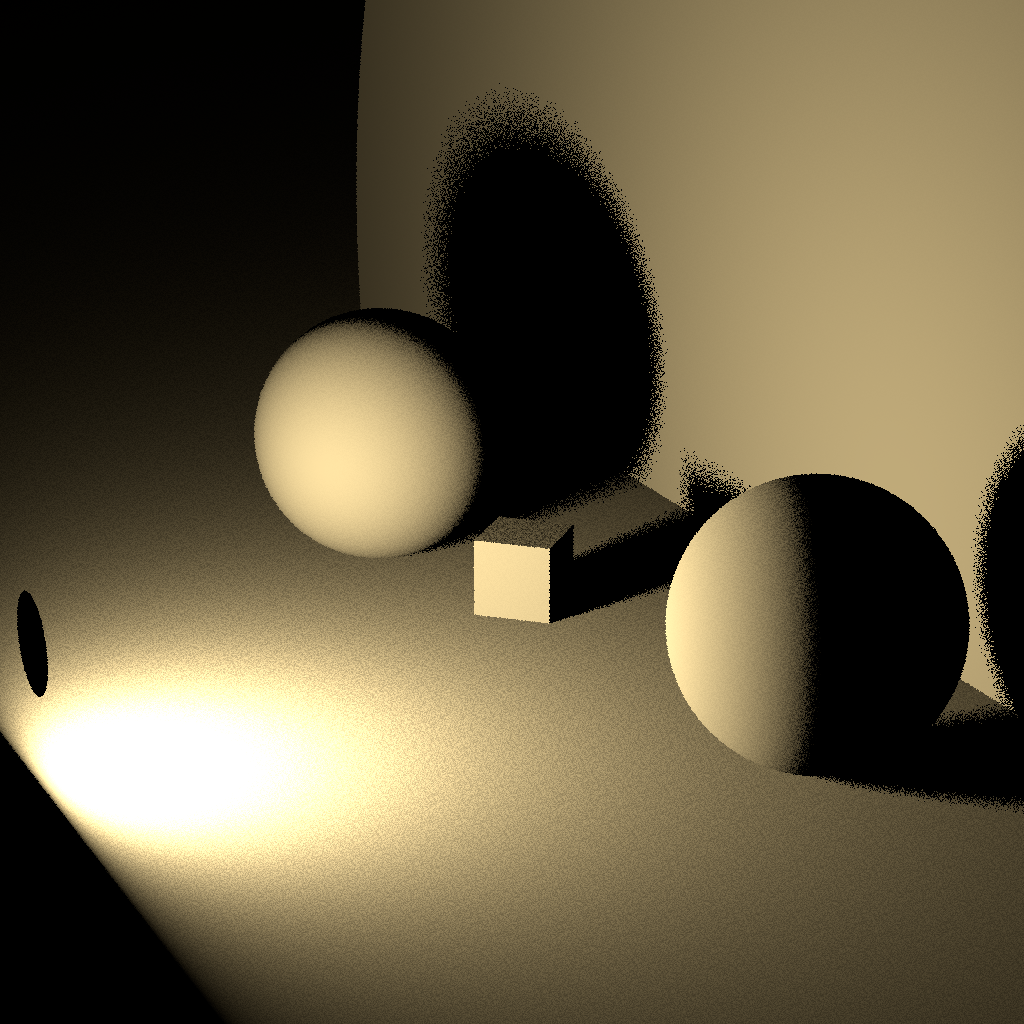
\includegraphics[width=\textwidth]{imagenes/rect9}
            \vspace{0.2cm}

            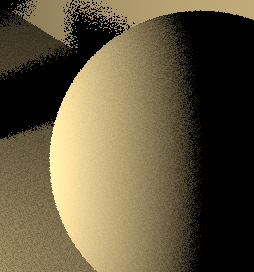
\includegraphics[width=\textwidth]{imagenes/rect91}
            \vspace{0.2cm}

            
\includegraphics[width=\textwidth]{imagenes/rect92}
            \caption{Mapa radial}
            \end{subfigure}% 
  \end{minipage}
  \begin{minipage}{\dimexpr .33\textwidth-\fboxsep-2\fboxrule}
   \begin{subfigure}{\textwidth}
            \centering
            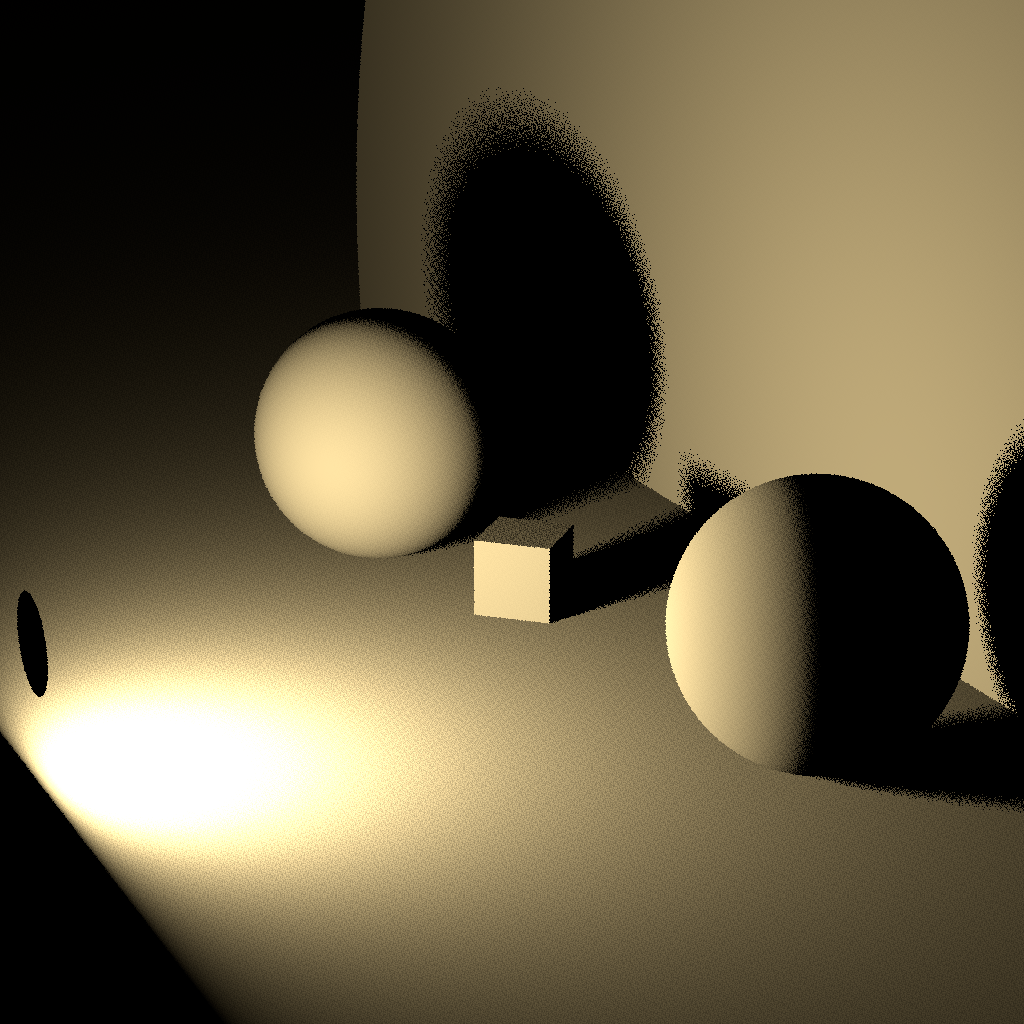
\includegraphics[width=\textwidth]{imagenes/rect10}
            \vspace{0.2cm}

            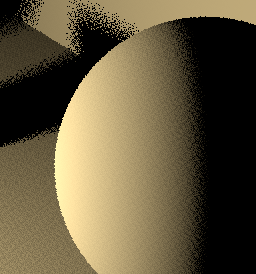
\includegraphics[width=\textwidth]{imagenes/rect101}
            \vspace{0.2cm}

            
\includegraphics[width=\textwidth]{imagenes/rect102}
            \caption{Mapa Paralelo}
            \end{subfigure}% 
  \end{minipage}}
  \fbox{\begin{minipage}{\dimexpr \textwidth-2\fboxsep-3\fboxrule}
    \abovecaptionskip=0pt
    \caption{Comparativa entre muestreo uniforme respecto al área, mapa radial y paralelo. Imágenes generadas con una muestra por píxel y con el algoritmo de iluminación directa.}
  \end{minipage}}
\end{figure}

\newpage

\begin{figure}[h!]
  \lineskip=-\fboxrule
  \fbox{\begin{minipage}{\dimexpr .5\textwidth-\fboxsep-2\fboxrule}
    \begin{subfigure}{\textwidth}
            \centering
            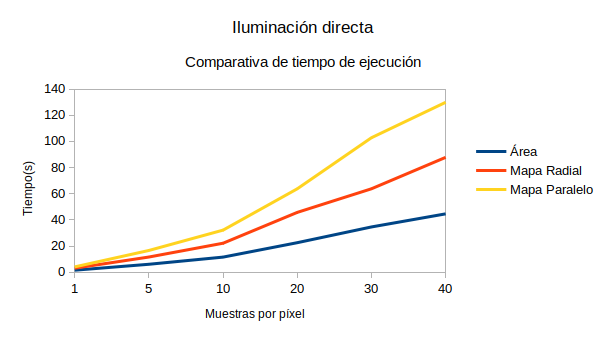
\includegraphics[width=\textwidth]{imagenes/compdl2}
            \caption{Iluminación Global}
            \end{subfigure} 
    \end{minipage}
    \hfill
    \begin{minipage}{\dimexpr .5\textwidth-\fboxsep-2\fboxrule}
            \begin{subfigure}{\textwidth}
            \centering
            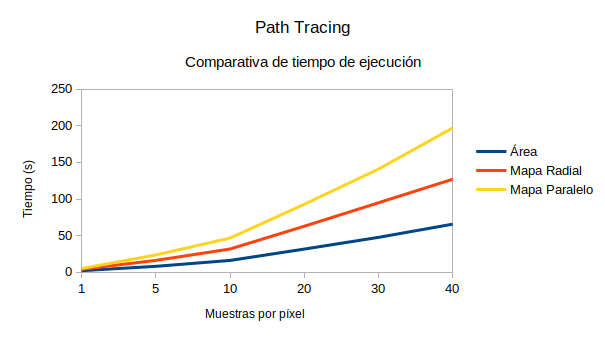
\includegraphics[width=\textwidth]{imagenes/comppath2}
            \caption{Path-tracing}
            \end{subfigure}  
    \end{minipage}}
  \fbox{\begin{minipage}{\dimexpr \textwidth-\fboxsep-2\fboxrule}
    \abovecaptionskip=0pt
    \caption{Comparativa del tiempo de ejecución.}
  \end{minipage}}
\end{figure}

\section{Muestreo de casquetes esféricos proyectados}

En esta sección presentaremos un método de muestreo para fuentes de luz esféricas, descrito en \cite{Urena2018}. Considerando la proyección $\rho$ definida en \ref{proyeccionAnguloSolido}, un casquete esférico proyectado es la imagen por $\rho$ de un casquete esférico sobre la esfera unidad. Fijado un punto $o\in\mathds{R}^3$ de la escena, consideramos $\pi_o$ la proyección sobre la esfera unidad con centro $o$. Consideramos también $\rho_o$ que es la proyección $\rho$ respecto a un sistema de referencia cuyo vector $z$ es la normal a la superficie en $P$, $n_o$. Dada una fuente de luz esférica $E$, nuestro objetivo es tomar muestras en el casquete esférico $\pi_o(E)$. Sin embargo, utilizaremos una distribución uniforme en el casquete esférico proyectado $\rho_o(\pi_o(E))$ para generar una muestra y dicha muestra se trasladará a $\pi_o(E)$ a través de $\rho_o^{-1}$. En vista de \ref{cambioProyectado}, concluimos que las muestras $\omega$ generadas según este procedimiento tendrán una función de densidad asociada:
$$f_{\omega}(\omega) = \frac{cos(\omega , n_o)}{A(\rho_o(\pi_o(E)))}\text{, }\forall \omega\in\pi_o(E)$$

donde $A(\rho_o(\pi_o(E)))$ es el área de $\rho_o(\pi_o(E))$. Este tipo de muestreo tiene una ventaja clave en el ámbito de la renderización fotorrealista. Supongamos que hemos generado $R$ muestras $\{\omega^{(r)}\}_{r=1}^R$, con función de densidad $f_{\omega}$, siguiendo una distribución uniforme en $\rho_o(\pi_o(E))$, con $E$ una fuente de luz cualquiera, y que queremos estimar la radiancia saliente en una dirección $\omega_s$ a causa de la radiancia incidente procedente de $E$. El estimador Monte Carlo que aproxima dicho valor de radiancia es el siguiente:
\begin{align*}
\frac{1}{R}\sum_{i=1}^R&\frac{L_e(t(o,\omega^{(i)}),-\omega^{(i)}) f(o,\omega_s,\omega^{(i)}) cos(n_o,\omega^{(i)}) }{f_{\omega}(\omega^{(i)})} = \\
\frac{1}{R}\sum_{i=1}^R&\frac{L_e(t(o,\omega^{(i)}),-\omega^{(i)}) f(o,\omega_s,\omega^{(i)}) cos(n_o,\omega^{(i)}) }{\frac{cos(\omega^{(i)} , n_o)}{A(\rho_o(\pi_o(E)))}} = \\
\frac{1}{R}\sum_{i=1}^R&L_e(t(o,\omega^{(i)}),-\omega^{(i)}) f(o,\omega_s,\omega^{(i)})  A(\rho_o(\pi_o(E)))
\end{align*}

Con lo que el estimador deja de tener el término coseno multiplicando. En el caso del muestreo uniforme respecto al ángulo sólido, dicho coseno hace que las muestras que estén cerca del horizonte acaben siendo menos relevantes. Por tanto, si las muestras siguen una distribución uniforme respecto al ángulo sólido proyectado, se reducirá la cantidad de muestras con poca aportación al estimador. Otra ventaja es que si el punto $o$ que estamos sombreando pertenece a una superficie difusa, es decir, si $f$ es constante en $o$, y si la cantidad de radiancia que emite la fuente de luz es constante en todos puntos y en todas direcciones, entonces con una sola muestra obtendremos el valor real de la radiancia saliente en cualquier dirección a causa de la radiancia incidente procedente de $E$ (basta ver la forma del estimador).

Pasamos ya a presentar los métodos de esta sección. Igual que en los casos anteriores, definiremos dos mapas $M_s:[0,1]^2\rightarrow \rho_o(\pi_o(E))$, $M_t:[0,1]^2\rightarrow \rho_o(\pi_o(E))$ que preserven el área. 

\subsection{Descripción del sistema de referencia y otros parámetros}
Consideramos los siguientes tres vectores, con $s$ el centro de la esfera $E$:
$$\overset{\wedge}{z} = n_o\hspace{1cm} y= \frac{(s-o)\times \overset{\wedge}{z}}{\|(s-o)\times \overset{\wedge}{z}\|} \hspace{1cm} x=\overset{\wedge}{z}\times y$$

En el caso en que el centro de la esfera esté en la misma dirección que $\overset{\wedge}{z}$, tomaremos $y$ cualquier vector perpendicular a $\overset{\wedge}{z}$. Consideremos el siguiente punto, que es la proyección de $s$ sobre la esfera unidad de centro $o$:
$$c=\frac{s-o}{\|s-o\|}$$

Y siendo $r$ el radio de la esfera, consideramos los dos siguientes ángulos (ver figura 5.6, izquierda):
$$\alpha = \arcsin(\frac{r}{\|s-o\|}) \hspace{1cm} \overset{\wedge}{\beta}=\arcsin(\overset{\wedge}{z}(c-o))$$

Vemos que $\overset{\wedge}{\beta}\in[-\pi/2,\pi/2]$. En el caso $\overset{\wedge}{\beta}<0$, tomaremos:
$$z = -\overset{\wedge}{z}\hspace{1cm} \beta = -\overset{\wedge}{\beta}$$

Y en caso de que $\overset{\wedge}{\beta}\geq 0$, tomamos:
$$z = \overset{\wedge}{z}\hspace{1cm} \beta = \overset{\wedge}{\beta}$$

El sistema de referencia que usaremos será $\{o;(x,y,z)\}$.

\begin{figure}[h]
  \lineskip=-\fboxrule
  \fbox{\begin{minipage}{\dimexpr \textwidth-2\fboxsep-2\fboxrule}
    \centering
    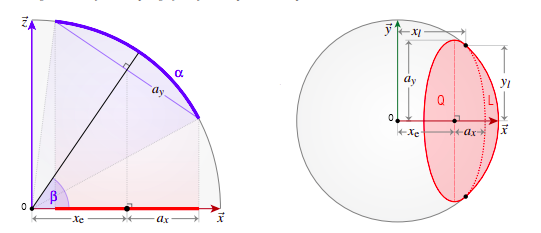
\includegraphics[width=0.9\textwidth]{imagenes/figura4_7}
  \end{minipage}}
  \fbox{\begin{minipage}{\dimexpr \textwidth-2\fboxsep-2\fboxrule}
    \abovecaptionskip=0pt
    \caption{Parametrización de la esfera $Q$ y la luna $L$.}
    \source{\cite{Urena2018}}
  \end{minipage}}
\end{figure}

Llegados a este punto tenemos que distinguir dos casos. Por un lado, si $0\leq\alpha\leq\beta$, significará que el casquete esférico $\pi_o(E)$ está completamente contenido en el hemisferio superior de la esfera unidad cuyo polo norte es $z$. En este caso, $\rho_o(\pi_o(E))$ será una elipse. Por otro lado, si $0\leq\beta<\alpha$, el casquete esférico tendrá una parte contenida en el hemisferio superior y otra en el hemisferio inferior. En este caso notaremos por $\rho_o(\pi_o(E))^+$ a la proyección de la parte de $\pi_o(E)$ contenida en el hemisferio superior, que tendrá forma de una elipse $Q$ unida con una luna $L$ (ver figura 5.6 derecha). Notaremos por $\rho_o(\pi_o(E))^-$ a la proyección de la parte de $\pi_o(E)$ contenida en el hemisferio inferior, que tendrá forma de luna $L$.

Vamos por tanto a calcular ciertos parámetros relacionados con la esfera $Q$ y con la luna $L$ (ver figura 5.6 derecha). Por un lado, la longitud de los semiejes de la elipse, $a_x$, $a_y$, y la coordenada $x$ del centro de la elipse, $x_e$, cumplen que:
$$a_y=\sin(\alpha) \hspace{1cm} a_x=\sin(\alpha)\sin(\beta) \hspace{1cm} x_e=\cos(\alpha)\cos(\beta)$$

Por otro lado, en el caso de que $0\leq\beta<\alpha$ y la luna $L$ esté definida, calcularemos los puntos de tangencia de la elipse con el disco, $(x_l,y_l)$, $(x_l,-y_l)$, haciendo uso de que cumplen las ecuaciones de la circunferencia y la elipse, obteniendo que:
$$x_l = \frac{\cos(\alpha)}{\cos(\beta)}\hspace{1cm} y_l=\sqrt{1-\frac{\cos^2(\alpha)}{\cos^2(\beta)}}$$

En el caso de que $0\leq\beta<\alpha$, tenemos que decidir en que hemisferio tomaremos muestras. Dado que partimos de una muestra uniforme en $[0,1]^2$, podemos usar cualquiera de las componentes para determinar que hemisferio muestrearemos, y la probabilidad de muestrear cada uno es proporcional al área relativa entre las dos proyecciones. Si el hemisferio muestreado es el inferior entonces cambiaremos el eje $z$ por $-z$. Una vez determinado el hemisferio muestreado, tenemos que transformar la muestra utilizada para que vuelva a cubrir el intervalo $[0,1]$.

\subsection{Construcción de la parametrización $M_s$}
Por la simetría de los tres tipos de proyección, podemos muestrear sólo en la parte de la proyección con componente $y$ positiva para luego ajustar la muestra en toda la proyección. En vista de la figura 4.7, definimos la siguiente función, que mide el área de una porción de la proyección de la esfera delimitada por un segmento paralelo al eje $x$:
$$A_p(s) = \int_0^s [x_{max}(r)-x_{min}(r)]dr $$

Distinguimos el caso $1$, donde muestreamos solo una elipse $Q$, el caso $2$, donde muestreamos una elipse y una luna, y el caso $3$, donde solo muestreamos la luna $L$. Entonces definimos $x_{max}$ y $x_{min}$ como:
\[ x_{min}(s) = 
   \begin{cases} 
     x_e-a_x\sqrt{1-\frac{s^2}{a_y^2}},  & \text{en el caso $3$}  \\
     x_e+a_x\sqrt{1-\frac{s^2}{a_y^2}},  & \text{en los casos $1$ y $2$}
   \end{cases}
  \]

\[ x_{max}(s) = 
   \begin{cases} 
       x_e+a_x\sqrt{1-\frac{s^2}{a_y^2}},  & \text{si $\alpha\leq\beta$ o si $y_l<s$} \\
       \sqrt{1-s^2}, & \text{si $\beta < \alpha$ y $s\leq y_l$}
   \end{cases}
\]

\begin{figure}[h]
  \lineskip=-\fboxrule
  \fbox{\begin{minipage}{\dimexpr \textwidth-2\fboxsep-2\fboxrule}
    \centering
    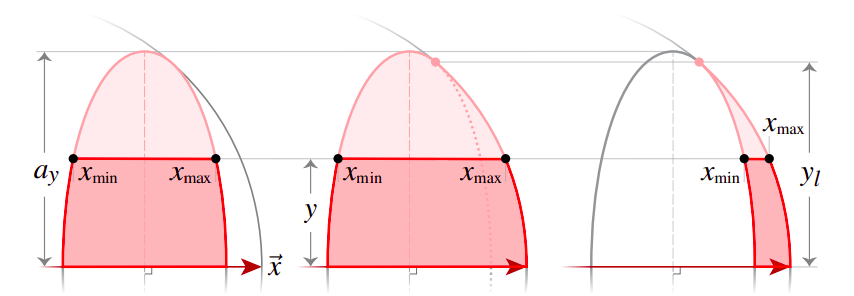
\includegraphics[width=0.9\textwidth]{imagenes/figura4_8}
  \end{minipage}}
  \fbox{\begin{minipage}{\dimexpr \textwidth-2\fboxsep-2\fboxrule}
    \abovecaptionskip=0pt
    \caption{Descripción del mapa $M_s$.}
    \source{\cite{Urena2018}}
  \end{minipage}}
\end{figure}

Entonces se cumple que, integrando la expresión anterior:
\[ A_p(s) = 
   \begin{cases} 
       2A_E(s),  & \text{en el caso 1} \\
       2A_E(s) + A_C(s') - A_E(s'),  & \text{en el caso 2} \\
       A_C(s') - A_E(s'),  & \text{en el caso 3} 
   \end{cases}
\]

donde $s'=\min\{y_l,s\}$, $I(u,w) = \frac{1}{2}(uw\sqrt{1-u^2} + \arcsin(u))$, y:
$$A_E(s) = a_xa_yI(\frac{s}{a_y},1)$$
$$A_C(s) = I(s,1)-x_es$$

Por último tomamos $v=(v_1,v_2)\in[0,1]^2$, y definimos:
\[ y_1 = 
   \begin{cases} 
      -y^*: A_p(y^*)-(1-2v_1)A_p(a_y)=0,  & \text{si $v_1<0.5$} \\
      y^*:  A_p(y^*)-(2v_1-1)A_p(a_y)=0,  & \text{si $v_1\geq 0.5$}
   \end{cases}
\]

$$x_1 = x_{min}(y_1) + v_2 (x_{max}(y_1) - x_{min}(y_1))$$

Para calcular el valor de $y_1$, utilizamos el método de Newton-Raphson. Por último la dirección buscada es:
$$M_s(v) = x_1\cdot x + y_1\cdot y + \sqrt{1-x_1^2-y_1^2} \cdot z.$$

$M_s$ preserva el área por como la hemos construido.

\subsection{Construcción de la parametrización $M_t$}
Fijamos $v=(v_1,v_2)\in [0,1]^2$. Como en el caso anterior, por simetría, sólo consideramos la parte con $y$ positiva del casquete esférico proyectado. En vista de la figura 5.9, consideramos una región delimitada por una línea radial, tal que dicha región preserve el área respecto a la primera variable de $v$. Dado un ángulo $\phi\in [0,\pi]$, el área de la región asociada al radio cuyo ángulo con el eje $x$ es $\phi$ viene dada por:
$$A_r(\phi) = \int_0^{\phi}\int_{r_{\min}(x)}^{r_{\max}(x)} r \text{ }dr dx = \frac{1}{2}\int_0^{\phi}(r_{\max}^2(x)-r_{\min}^2(x))\text{ } dx$$

donde se ha usado que se trata una integral en coordenadas polares.

\begin{figure}[h]
  \lineskip=-\fboxrule
  \fbox{\begin{minipage}{\dimexpr \textwidth-2\fboxsep-2\fboxrule}
    \centering
    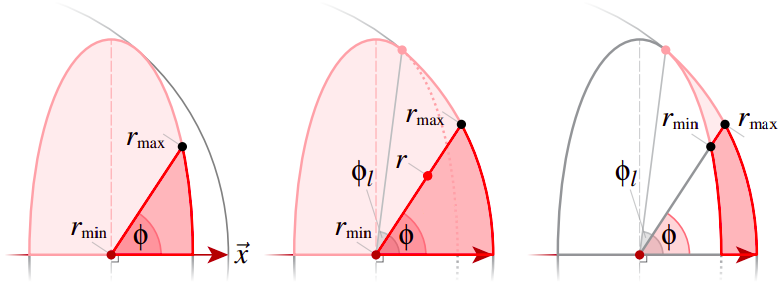
\includegraphics[width=0.9\textwidth]{imagenes/figura4_9}
  \end{minipage}}
  \fbox{\begin{minipage}{\dimexpr \textwidth-2\fboxsep-2\fboxrule}
    \abovecaptionskip=0pt
    \caption{Descripción del mapa $M_t$.}
    \source{\cite{Urena2018}}
  \end{minipage}}
\end{figure}

 Al igual que en el mapa $M_s$, distinguimos tres casos, el caso $1$, donde muestreamos solo una elipse $Q$, el caso $2$, donde muestreamos una elipse y una luna, y el caso $3$, donde solo muestreamos la luna $L$. Entonces definimos $r_{max}$ y $r_{min}$ como:
\[ r_{min}(\phi) =
   \begin{cases}
      0, & \text{en los casos 1 y 2}, \\
      \frac{a_x}{\sqrt{1-\cos^2\beta\sin^2\phi}}, & \text{en el caso 3}
   \end{cases}
  \]

\[ r_{max}(\phi) =
   \begin{cases}
      \frac{a_x}{\sqrt{1-\cos^2\beta\sin^2\phi}}, & \text{si }\alpha\leq\beta \text{ o si } \phi_l\leq\phi,\\
      \sqrt{1-x_e^2\sin^2\phi}-x_e\cos\phi, & \text{si } \beta< \alpha \text{ y } \phi < \phi_l.
   \end{cases}
  \]

donde $\phi_l=\arctan(\frac{y_l}{x_l-x_e})$. Integrando la expresión anterior obtenemos:
\[ A_r(\phi) =
   \begin{cases}
      A_E'(\phi), & \text{caso 1}, \\
      A_E'(\phi) - A_E'(\phi') + A_C'(\phi')  , & \text{caso 2}, \\
      A_C'(\phi') - A_E'(\phi'), & \text{caso 3} 
   \end{cases}
  \]

donde $\phi' = \min(\phi, \phi_l)$ y:
\[ A_E'(\phi) =
   \begin{cases}
        \frac{1}{2}a_xa_y\arctan(\frac{a_x}{a_y}\tan(\phi)), & \text{si $\phi\leq \pi/2$}\\
        \pi + \frac{1}{2}a_xa_y\arctan(\frac{a_x}{a_y}\tan(\phi)), & \text{si $\phi > \pi/2$}
   \end{cases}
   \]
   
$$A_C'(\phi) = I(\sin(\phi),x_e^2)-I(x_e\sin(\phi),1)$$

con $I$ la función definida en el apartado anterior. Por último definimos:
\[ \phi_1 = 
   \begin{cases} 
      -\phi^*: A_r(\phi^*)-(1-2v_1)A_p(\pi)=0,  & \text{si $v_1<0.5$} \\
      \phi^*:  A_r(\phi^*)-(2v_1-1)A_p(\pi)=0,  & \text{si $v_1\geq 0.5$}
   \end{cases}
\]

$$r_1 = \sqrt{r_{min}^2(\phi_1) + v_2 (r_{max}^2(\phi_1) - r_{min}^2(\phi_1))}$$

Para calcular el valor de $\phi_1$, utilizamos el método de Newton-Raphson. $r_1$ está definida de esta forma para que el mapa preserve el área. Por último, tomando $x_1 = (x_e + r_1\cos(\phi_1))$, $y_1 = (r_1\sin(\phi_1))$, la dirección buscada es:
$$M_t(v) = x_1\cdot x + y_1\cdot y + \sqrt{1-x_1^2-y_1^2} \cdot z.$$


Sin embargo, en el caso $1$ en que solo tenemos una elipse, el muestreo se puede optimizar tomando $x_1=x_e + a_x\sqrt{v_1}\cos(2\pi v_2)$, $y_1= a_y\sqrt{v_1}\sin(2\pi v_2)$, y definiendo el mapa $M_t$ como:
$$M_t(v) = x_1\cdot x + y_1\cdot y + \sqrt{1-x_1^2-y_1^2} \cdot z.$$


\subsection{Resultados obtenidos}



%%\chapter{Conclusiones y Trabajos Futuros}
%
%

\nocite{*}
\bibliography{bibliografia/bibliografia}\addcontentsline{toc}{chapter}{Bibliografía}
\bibliographystyle{alpha}
%\printbibliography
%\addcontentsline{toc}{chapter}{Bibliografía}
%\bibliographystyle{numeric}

%\appendix
%\input{apendices/manual_usuario/manual_usuario}
%%\input{apendices/paper/paper}
%\input{glosario/entradas_glosario}
% \addcontentsline{toc}{chapter}{Glosario}
% \printglossary
%\thispagestyle{empty}

\end{document}
